% What is the domain // what is the current use // what are the current problems // what are the technical challenges // how did i meet these technical challenges // how did it work

\chapter{Iterative Appliation Design (contributions)}
\label{cha:contributions}

This chapter describes the contributions of the papers that are included in this thesis in four different application domains.  This first section describes the separation of papers into the topic areas and the subsequent sections contain each a description of the problem domain and then elaborate on the contributions of the papers included in the topic.

\section{Overview} \label{contributions:overview}

\textbf{Finite Element Models. } \paperef{paperA} deals with algorithmic challenges to efficiently render non-linear finite element models, in this case exemplified on a high-resolution simulation of stress inside a heart muscle, a deformation model of the breast, and a simultion of the muscle fibers in the tongue~(\SC{contributions:fem}).

\textbf{Deep Brain Stimulation. } \paperef{paperB} describes an application system that is targeted to be used in deep brain stimulation interventions in order improve the placement of electrodes using a fusion of multiple data modalities in real-time~(\SC{contributions:dbs}).

\textbf{Urban Search \& Rescue. } \paperef{paperC}, \paperef{paperD}, and \paperef{paperE} describe the collaborative work on designing a visualization system to support urban search \& rescue operators and rescuers during the reconnaissance of partially collapsed buildlings.  The system utilizes acquired \nD{3} point cloud data as the basis for a path suggestion algorithm, whose results are presented to the expert user for a human-in-the-loop decision support of optimal building exploration in search for victims.~(\SC{contributions:usar})

\textbf{Astrophysical Visualization. } The papers in this topic deal with visualization systems that were design in the context of astronomical and astrophysical phenomena. \paperef{paperF} and \paperef{paperG} describe visualization systems that are applied to space weather and ion simulations respectively, \paperef{H}, \paperef{I}, \paperef{J} describe the development of \emph{OpenSpace}, an open-source visualization framework enabling the public dissemination of astronomical data.~(\SC{contributions:astro})

Each of the topics provides a short introduction into the domain and, then, elaborate on the work that has been done in the respective papers.

% For each contribution explain:
%   Problem domain
%   System that solves the problem
%   Collaboration with the experts
%   Evaluations
%   Generalizability (future work?)

% \section{Biological and Medical Systems} \label{contributions:medbio}



% \begin{itemize}
% \item Describe background and previous work in biological visualization + systems
% \item Describe background and previous work in medical visualization + systems
% \item Medical visualization as one of the first expert domains
% \item Support for the operating theater
% \item General problems with medical visualization
% \begin{itemize}
%     \item Hard to convince people to use it:
%     \item Certification / limited time of the physicians
% \end{itemize}
% \item More information about medical visualization \cite{preim2007visualization}
% \end{itemize}

\section{Finite Element Models} \label{contributions:fem}
The work described in \paperef{paperA} was developed in the context of creating an algorithm to efficiently render non-linear finite element models that traditionally require expensive calculations during the rendering to be represented correctly.  The papers published describe an algorithm that utilizes an efficient storage and look-up of precalculated rays, improving the rendering performance by an order of magnitude.

\subsection{Domain and Scientific Problems} \label{contributions:fem:background}
Finite element models~(FEM)~methods are used extensively in a large number of fields, for example engineering, construction, or biology, as an approach to solve complex problems numerically by separating the problem domain into a finite number of cells over which the numerical simulation can be performed efficiently.  The problem domain is subdivided into a fixed number of cells, each with their own local coordinate systems.  Two coordinate system are associated with each element; the location and deformation of an element is specified in Cartesian \emph{world coordinates}, whereas the computed values of the element are represented in a material coordinate system $\xi$ which, in most cases, is not Cartesian but can be of arbitrary geometry that simplifies the underlying computation (see Figures~\ref{contributions:fem:rays:world} and \ref{contributions:fem:rays:xi}).  The vertex coordinates of each element can be expressed in either coordinate system through a bilinear transformation; in many cases, however, an analytical solution does not exist for arbitrary coordinates and the transform involves computationally expensive iterative solvers, such as the Newton method.  For more information on finite element models, we refer the reader to the book by Bathe and Wilson~\cite{bathe1976numerical}.

\begin{figure}
\centering
\begin{subfigure}[b]{0.3\textwidth}
    \fbox{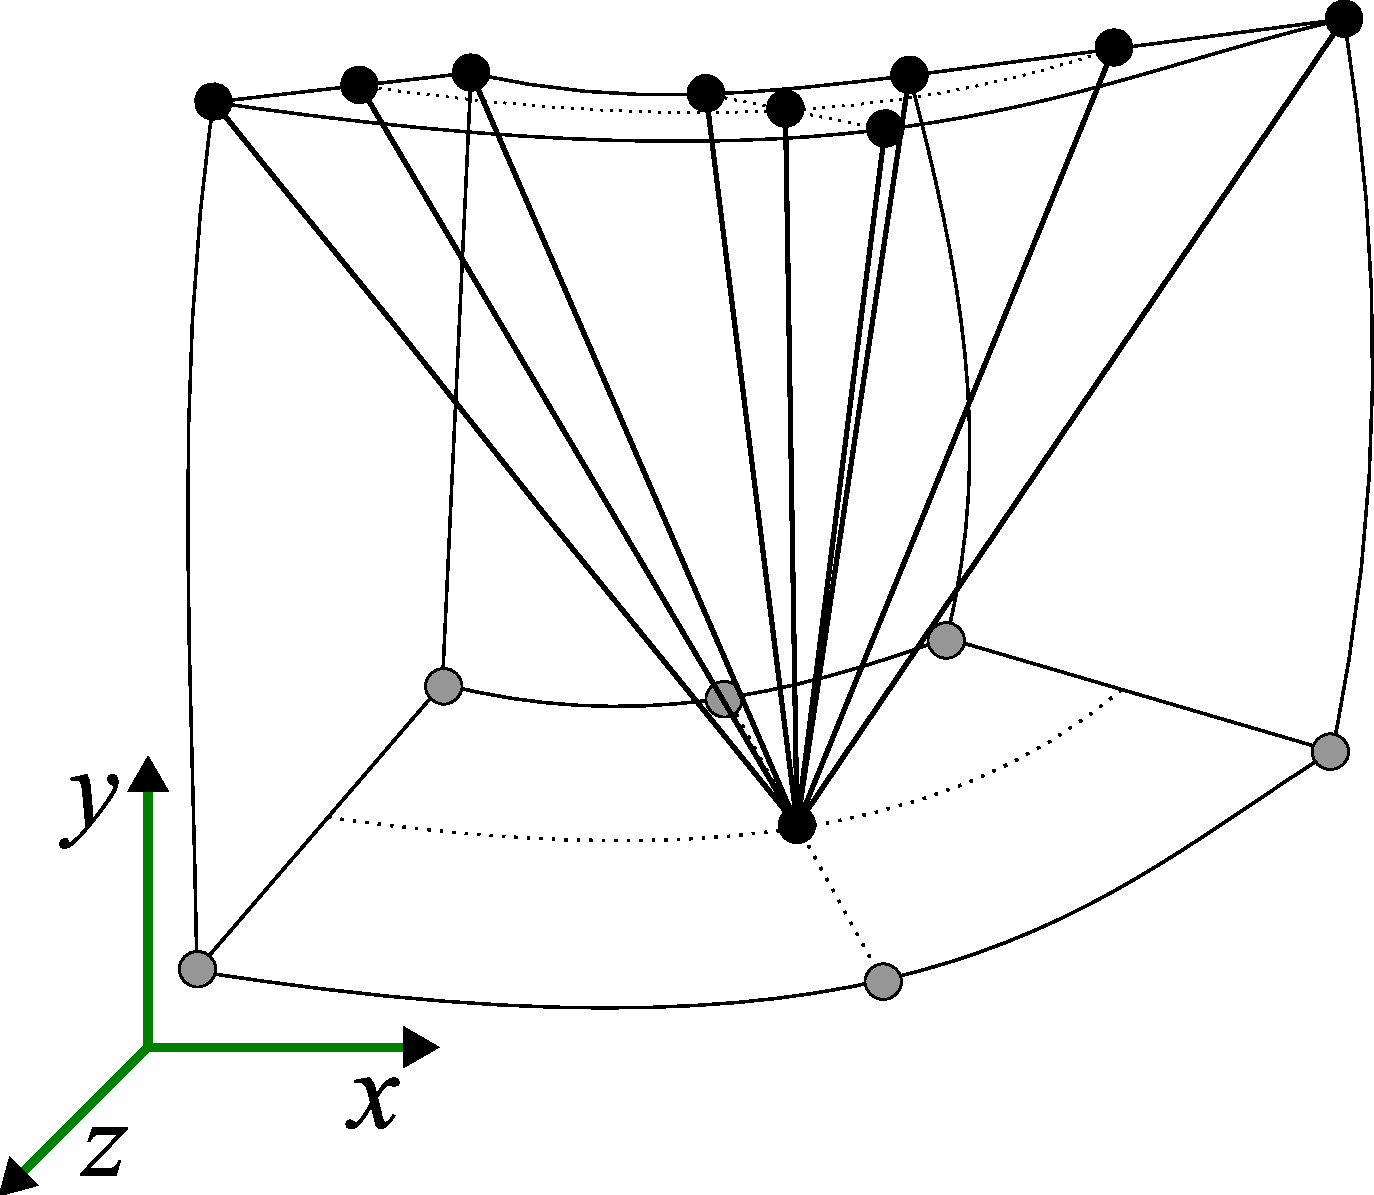
\includegraphics[width=0.99\textwidth, height=4cm]{figures/contributions/fem/splines-world-space.pdf}}
    \caption{Rays and geometry shown in Cartesian world space}
    \label{contributions:fem:rays:world}
\end{subfigure}
\hfill
\begin{subfigure}[b]{0.3\textwidth}
    \fbox{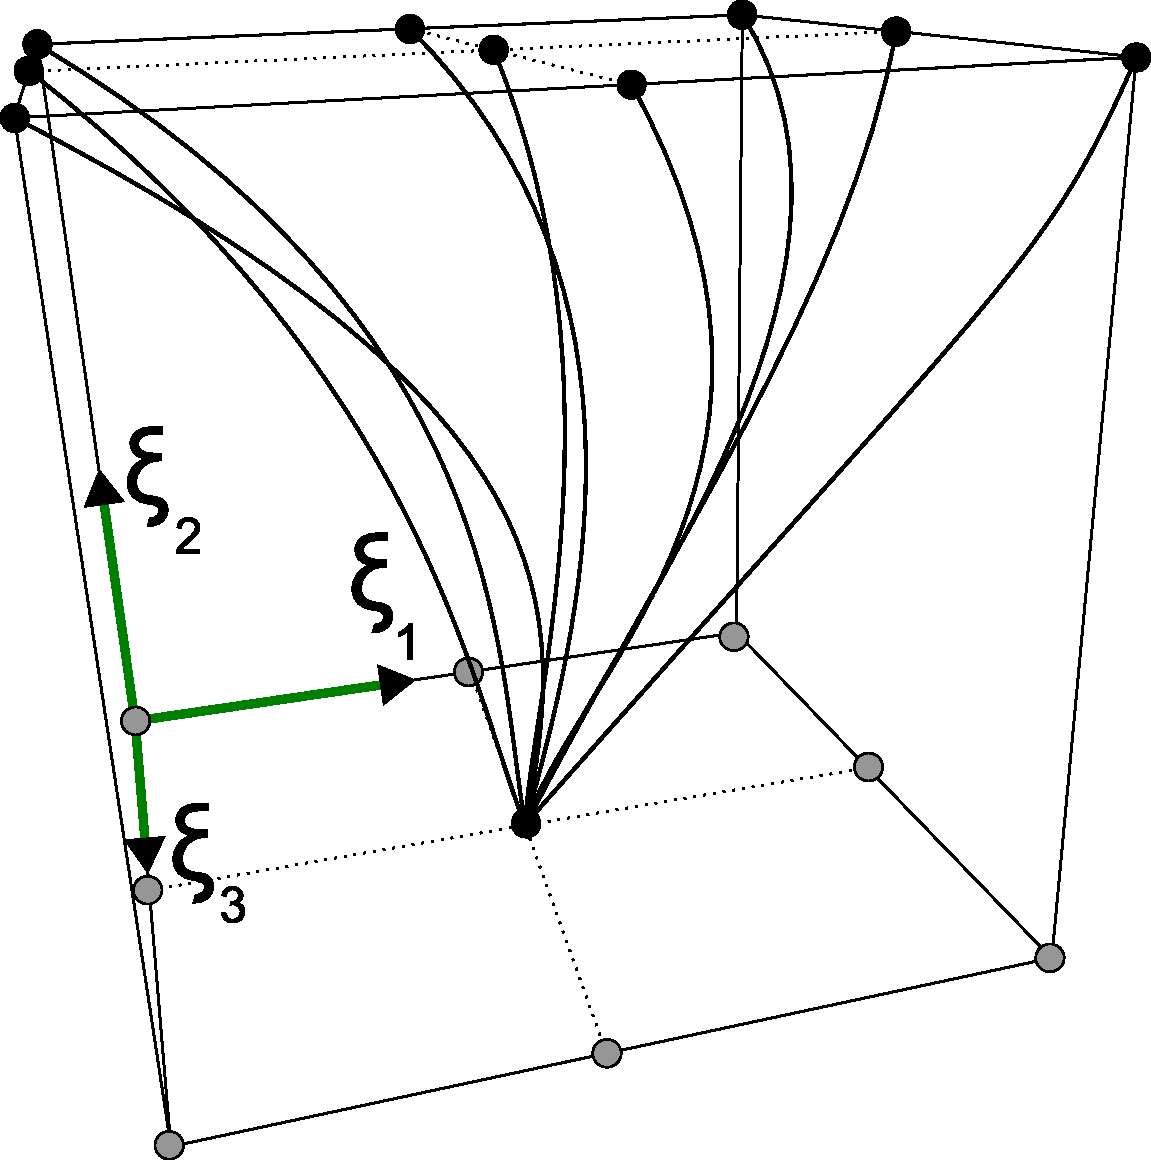
\includegraphics[width=0.99\textwidth, height=4cm]{figures/contributions/fem/splines-xi-space.pdf}}
    \caption{Rays and geometry shown in material space}
    \label{contributions:fem:rays:xi}
\end{subfigure}
\hfill
\begin{subfigure}[b]{0.3\textwidth}
   \fbox{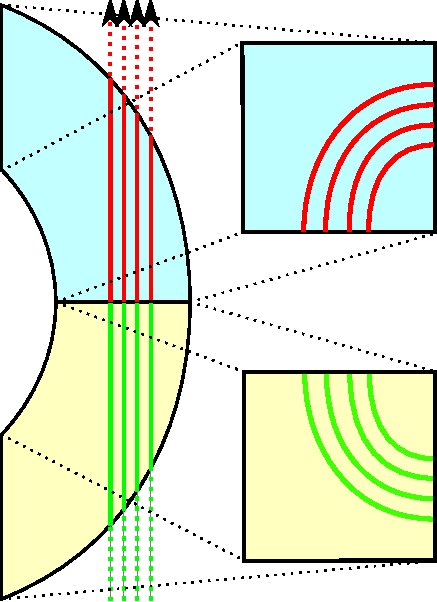
\includegraphics[width=0.99\textwidth, height=4cm]{figures/contributions/fem/viewingrays.pdf}}
   \caption{Converting between coordinate systems converts the straight viewing rays into curved rays}
   \label{contributions:fem:rays:rays}
\end{subfigure}
\caption{These images demonstrate the transformation between world coordinates and material coordinates for a set of viewing rays when viewing the element geometry and the viewing rays from the world (a) or the material (b) coordinate system.}
\label{contributions:fem:rays}
\end{figure}

This work was mainly developed in the focus of a simulation of a human heart that calculates the stress tensor at each location during the cardiac cycle.  By comparing the results of healthy and abnormal hearts, it is possible to detect structural defects before they manifest~\cite{young1992three, young1995tracking}. Traditionally, these models have been visualized using iso-surfaces or glyphs~\cite{wunsche2003visualization}, but not using volume raycasting.

When performing volume raycasting on the FEM dataset, view rays for each pixel are defined in world coordinates and are straight lines in world coordinates.  For each element that is intersected by a ray, all rays have to be converted into the material space in order to sample the values in $\xi$ material space.  \fref{contributions:fem:rays:rays} shows an example of the ray transformations from a Cartesian world space into a bicubic-linear material space.  Converting each sample point from Cartesian space into material space using an iterative solver is prohibitively expensive for real-time use.


\subsection{Application Requirements} \label{contributions:fem:requirements}
For each viewing ray, a potentially large number of sampling points have to be retrieved for a correct front-to-back composited image that is free of artifacts.  The additional coordinate transform during the data access becomes a bottleneck in the case of non-linear FEM datasets, which reduces rendering speeds to non-interactive framerates.  \paperef{paperA} describes an algorithm that utilizes a precomputation step to cache a reduced set of possible rays that are then used in the rendering step to efficiently access the data, resulting in a $15\times$ performance gain, relative to straight-forward GPU implementations, which in turn, are an improvement of 2 to 4 orders of magnitude compared to a CPU implementation~\cite{liu12gpu}.




% The algorihtm described in \paperef{paperA} utilizes a preprocessing step, during which a large number of potential rays are calculated through all elements of the model.  The rays are represented using Catmull-Rom splines, the control points of which are stored ~\cite{catmull1974class}



\subsection{Algorithm} \label{contributions:fem:algorithm}
\begin{figure}
\centering
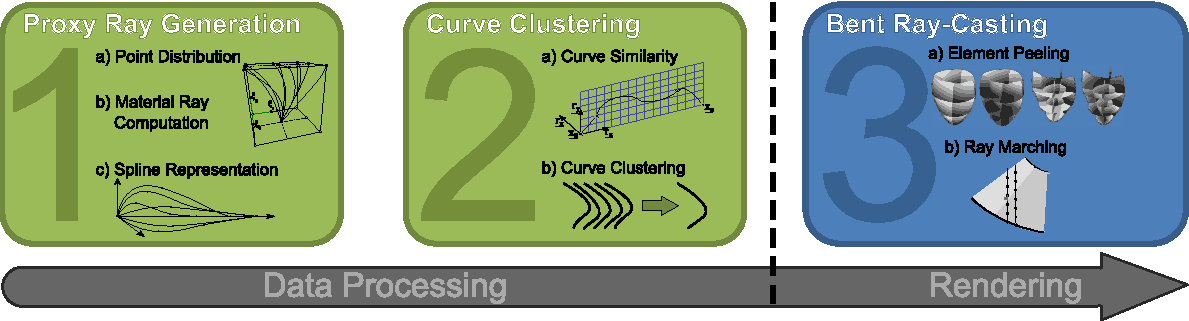
\includegraphics[width=\textwidth]{figures/contributions/fem/workflow.pdf}
\caption{The workflow employed in the finite element model volume rendering algorithm.  The first two steps are precomputing potential ray paths through the volume that increase the performance during the third step.}
\label{contributions:fem:workflow}
\end{figure}

In order to improve the performance of the rendering, the expensive coordinate transformations have to be computed off-line prior to the rendering and then retrieved efficiently.  The algorithm developed for \paperef{paperA} utilizes a Catmull-Rom spline based representation of the rays and $\xi$ material space, which can be efficiently stored and retrieved at rendering time~\cite{catmull1974class}.  A number of approximation steps are performed in order to increase the similarity between different rays and represent these by a reduced set of \emph{proxy rays}, which drastically reduces the number of rays that need to be stored and still maintain an artifact-free rendering.  \fref{contributions:fem:workflow} shows the workflow of the algorithm in detail, with the first two steps being precomputed once for each finite element model in order to improve the performance of the third real-time rendering step.

The algorithm consists of 5 steps, which are described in the following sections:
\begin{description}[leftmargin=10em,style=nextline]
  \item[Point Generation]  A fixed number of points are generated for each face of each element.  For each point, a \emph{proxy ray} is created to every other point that is in the same element but not the same face.
  \item[Ray computation]  The \emph{proxy rays} for each entry-exit point pair is sampled using a fixed sampling rate that is independent from the rendering sampling rate.  For each point, the expensive coordinate transformation is performed).
  \item[Curve Similarity] Through renormalization and alignment, the similarity between all \emph{proxy rays} is improved.
  \item[Curve Clustering] Using a K-Means algorithm, a representative subset of \emph{proxy rays} is crated.  Each original entry-exit point pair references the new representative path.
  \item[Rendering ]       For each viewing ray, the \emph{proxy rays} are used to sample the correct locations in material space without the need for the expensive coordinate transformaition.
\end{description}

The following two sections describe the method used in the curve clustering and the rendering;  the point generation and the ray computation steps are described in \paperef{paperA}.

% \subsubsection{Proxy Ray Generation} \label{contributions:fem:proxyray}
% First, we do not store the entirety of a proxy ray, but sample it in a few points and use these as control points for a Catmull-Rom spline from which we can reconstruct the original path. The number of control points that are used to approximate each ray is a user-defined parameters. The optimal parameter for this value depends on the complexity of the dataset (see \SC{contributions:fem:results}). 

% Second, we compute only a finite number of proxy rays for each element by creating a uniform grid on each of the elements surface and computing all proxy rays between pairwise combinations of grid points. Figures~\ref{contributions:fem:rays:world} and~\ref{contributions:fem:rays:xi} show a potential set of these rays for an element in world coordinates and material space. We can apply this approximation since well-behaved finite element simulations usually do not produce degenerate elements for which a much higher resolution is needed.


\subsubsection{Curve Clustering} \label{contributions:fem:curves}
\begin{figure}
\centering
\fbox{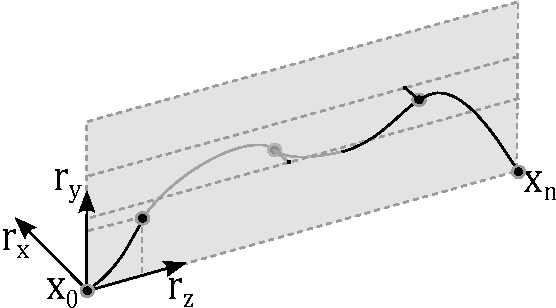
\includegraphics[width=0.99\textwidth]{figures/contributions/fem/splinetransformation.pdf}}
\caption{Increasing the similarity between splines through a lossless conversion into a common coordinate system.}
\label{contributions:fem:splines}
\end{figure}



A straight-forward sampling of the $|F|$ faces of the $|E|$ elements of the model using $n$ points per face results in $r_t = \left( n^2 \cdot |F| \right) ^2 \cdot |E|$ proxy rays.  Without a further reduction this number is prohibitely large for usage on the GPU.  However, since there is a potential for a high degree of similarity between rays due to symmetries and bounded ray complexity, we can utilize a clustering algorithm to reduce the number of representative \emph{proxy rays} necessary during the rendering without introducing large errors.

\begin{figure}
\centering
\begin{subfigure}[b]{0.4\textwidth}
    \fbox{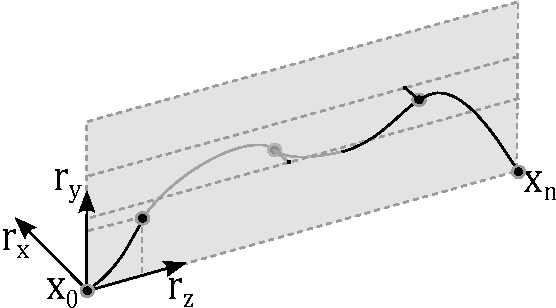
\includegraphics[width=0.99\textwidth]{figures/contributions/fem/splinetransformation.pdf}}
    \caption{Increasing the similarity between splines by converting them into a common coordinate system.}
    \label{contributions:fem:splines}
\end{subfigure}
\hspace{2cm}
\begin{subfigure}[b]{0.4\textwidth}
    \fbox{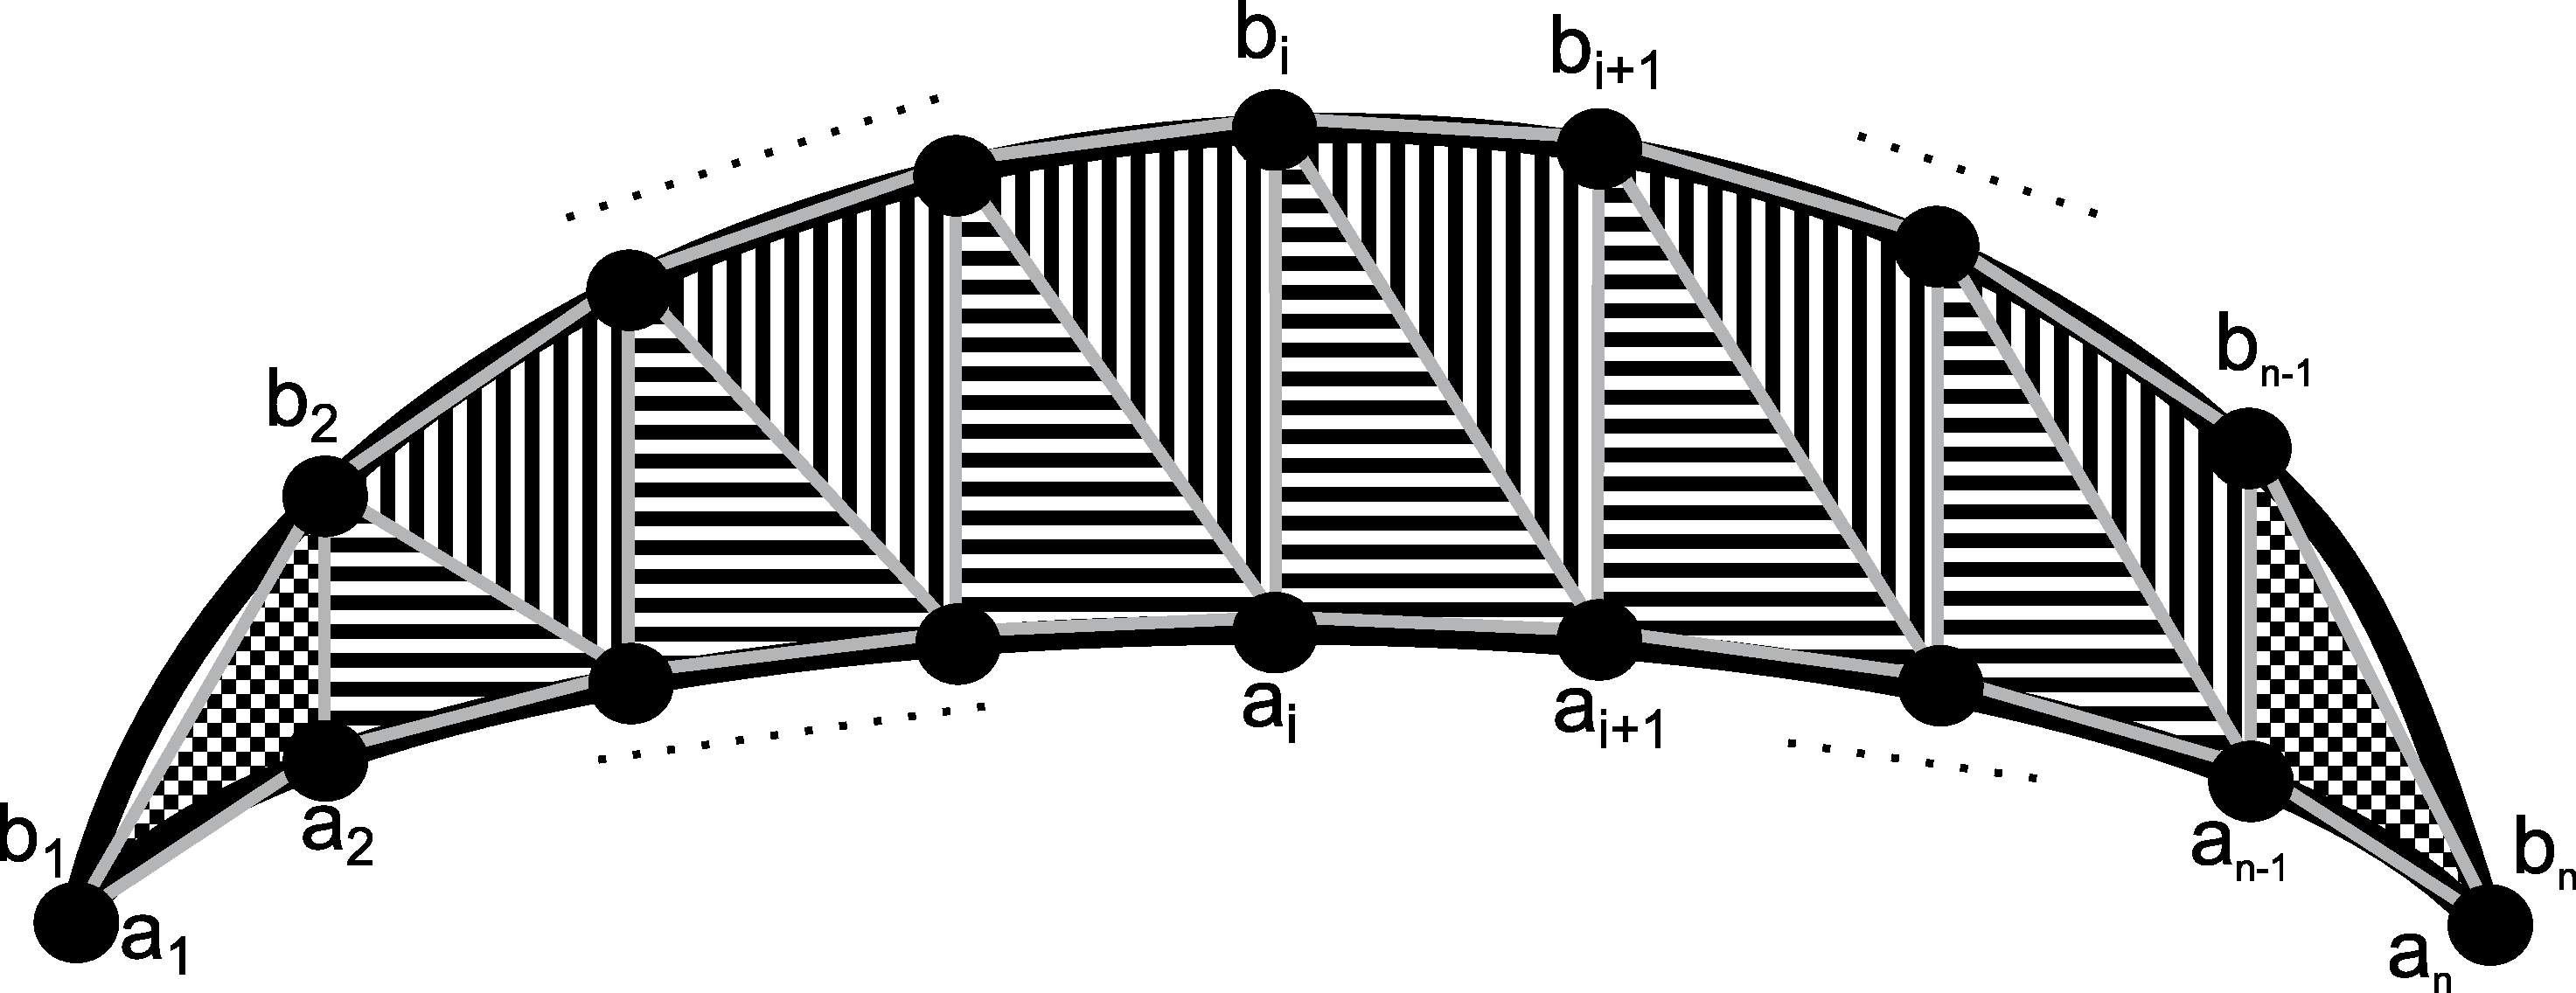
\includegraphics[width=0.99\textwidth]{figures/contributions/fem/metric.pdf}}
    \caption{A representation of the metric that is used in the K-Means clustering algorithm, approximating the area between the two rays by a sum of the triangle areas.}
    \label{contributions:fem:metric}
\end{subfigure}
\end{figure}

The first step is to increase the similarity between proxy rays while maintaining the ability to uniquely reconstruct the final ray.  For this, all rays are rotated and stretched such that the first point $P_1$ is equal to $(0,0,0)$ and the last $P_n$ control point is equal to $(0,0,1)$.  Then, all control points are rotated by a rotation angle $\theta$ around the $z$ axis such that the first point $P_i$ that is not collinear with $P_1$ and $P_n$ is in the $yz$ plane.  \fref{contributions:fem:splines} shows the results of these transformations on an example ray.  Both the translation and the scaling can then later be undone during the rendering without storing additional information, as the entry and exit points (and their distance) are known.  Only the angle $\theta$ needs to be recorded for each $\emph{proxy ray}

\begin{figure}
\centering
\fbox{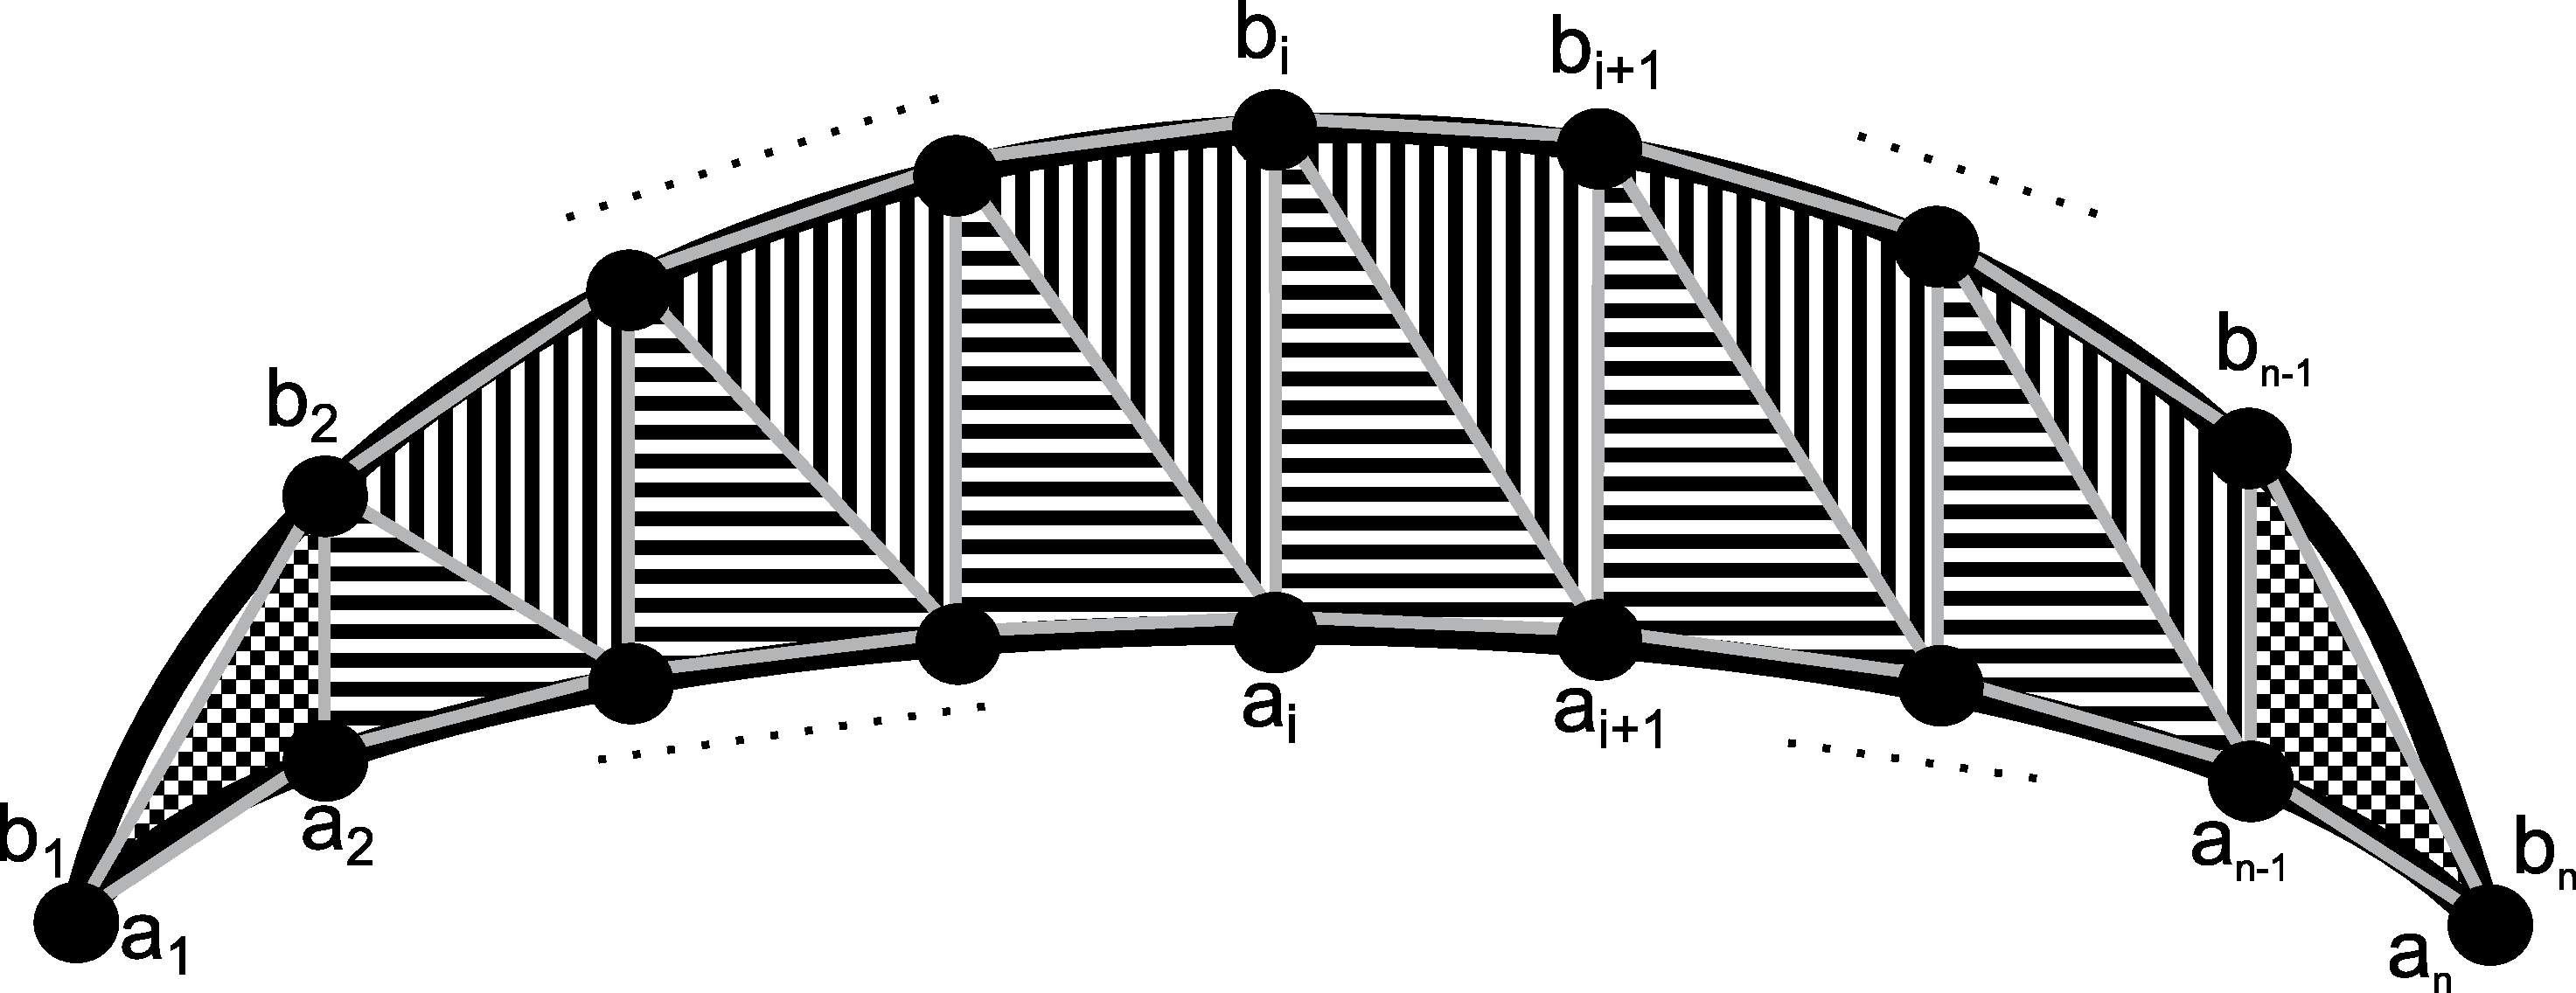
\includegraphics[width=0.99\textwidth]{figures/contributions/fem/metric.pdf}}
\caption{A representation of the metric that is used in the K-Means clustering algorithm, approximating the area between the two rays by a sum of the triangle areas.}
\label{contributions:fem:metric}
\end{figure}

For the clustering of the splines, we make use of the variant of the K-Means~\cite{hartigan75kmeans} algorithm because of its stability and ability to deal with values of arbitrary dimensions.  For this, we adapt an idea from Abraham~\etal \cite{abraham03clustering} and perform the clustering on the control points of the Catmull-Rom splines directly.  The metric for the clustering uses the area between two curves as approximated by a Riemann sum of triangles connecting the proxy rays, sampled at a high frequency (see~\fref{contributions:medbio:fem:metric}).  For two proxy rays $a$ and $b$, and their $n$ sampled points $a_1, \dots a_n$ and $b_0, \dots b_n$ with $a_1 = b_1$, $a_n = b_n$, $\exists i\in[2, n-1] : a{_i}_x = 0$, and $\exists j\in[2, n-1] : b{_j}_x = 0$ due to the transformation performed in the last paragraph, the similarity metric is defined by:

\begin{eqnarray}
d(a,b) &=& \frac{1}{2} \Big( \Vert a_1a_2 \times a_2b_2\Vert + \nonumber \\
&& \sum_{i=2}^{n-2}\Vert a_ia_{i+1} \times a_ib_i \Vert + \Vert b_ib_{i+1} \times b_{i+1}a_{i+1}\Vert + \\
&& \Vert a_{n-1}a_n \times a_{n-1}b_{n-1}\Vert \Big) \nonumber 
\end{eqnarray}

After applying the clustering, for each original point we now have a cluster identifier for the representative ray and the angle $\theta$ as computed above.



\subsubsection{Rendering} \label{contributions:fem:rendering}
\begin{figure}
    \centering
    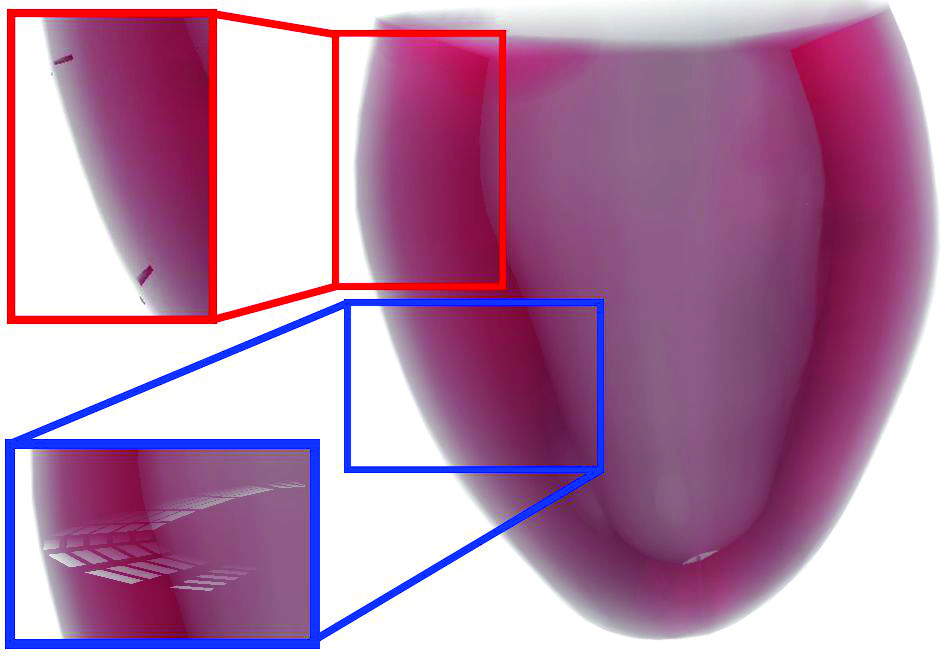
\includegraphics[width=0.5\textwidth]{figures/contributions/fem/heartfine.jpg}
    \caption{The insets show potential rendering artifacts when applying the depth peeling algorithm to finite element methods.}
    \label{contributions:fem:peeling}
\end{figure}
During the rendering step of the algorithm, the proxy geometries for all elements of the finite element model are rendered.  The material space coordinates are mapped to the RGB channel, as described by Kr\"uger and Westermann~\cite{kruger2003acceleration}, and the face identifier and element identifier are encoded in the transparency channel.  The entire scene is then rendered in multiple passes, employing a modified depth peeling approach as described by Everitt~\cite{everitt2001interactive} for each rendering pass.

\begin{wrapfigure}{o}{0.4\textwidth}
\centering
\fbox{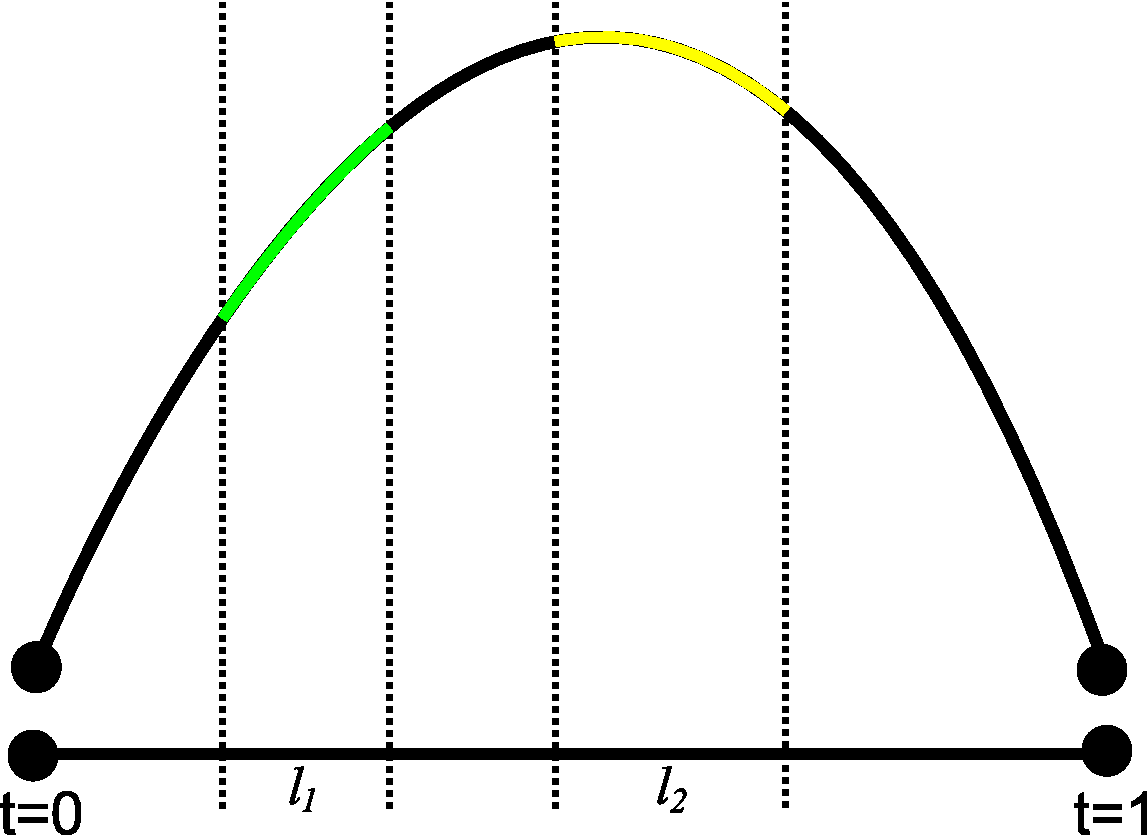
\includegraphics[width=0.99\textwidth]{figures/contributions/fem/arclength.pdf}}
\caption{The desire to uniformly sample the view ray in world space requires an arclength parametrization of the proxy ray.}
\label{contributions:fem:arclength}
\end{wrapfigure}

For each of the peeling rendering steps, we can then use the color information for each pair of fragments to retrieve the entry and exit points as well as the face and element ID. Using this information, we can retrieve the cluster ID and the angle $\theta$ of the proxy ray that belongs to the fragment pair.  The previous transformations of the proxy ray can be undone by scaling the proxy ray by the distance between the entry and exit points in world coordinates, translating and rotating the ray such that $P_1$ coincides with the entry point and $P_n$ coincides with the entry point, and finally rotating the proxy ray by $\theta$ around the axis connecting $P_0$ and $P_n$.

\begin{wrapfigure}{o}{0.4\textwidth}
\centering
\fbox{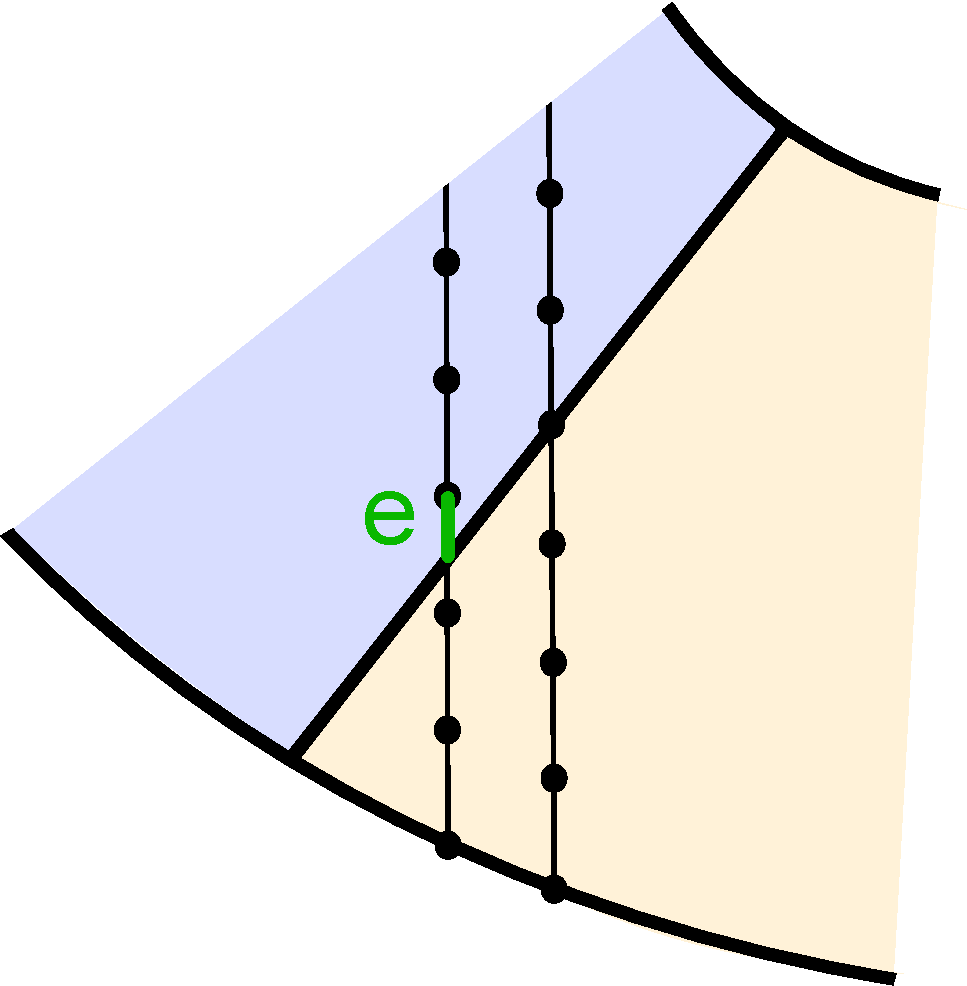
\includegraphics[width=0.99\textwidth]{figures/contributions/fem/overshoot.pdf}}
\caption{Special border handling is required between elements, as a na\"{i}ve implementation would oversample the boundary.}
\label{contributions:fem:overshoot}
\end{wrapfigure}


The ray marching can then interpolate along the Catmull-Rom spline to retrieve the correct sampling value in material space.  This ray marching cannot, however, take place in the material space as this would lead to a non-uniform sampling in world space (see~\fref{contributions:fem:arclength}). T herefore, the spline interpolation parameter $t \in [0,1]$ has to be converted into an arclength parametrization such that the sampling in material space becomes non-uniform to make the world space sampling uniform instead~\cite{guenter90arclength}.  A second subtle error occurs at the boundary between elements and is exemplified in~\fref{contributions:fem:overshoot}.  Restarting the ray marching at each element would also lead to a non-uniform sampling and thus rendering artifacts.  For this reason, the remaining distance between the last sample and the exit point is stored at the end of the ray marching and this distance is used to offset the first sampling point in the following element, similar to the method employed by Ljung \etal~\cite{ljung2006adaptive}.

\begin{figure}
\centering
\begin{subfigure}[b]{0.4\textwidth}
    \fbox{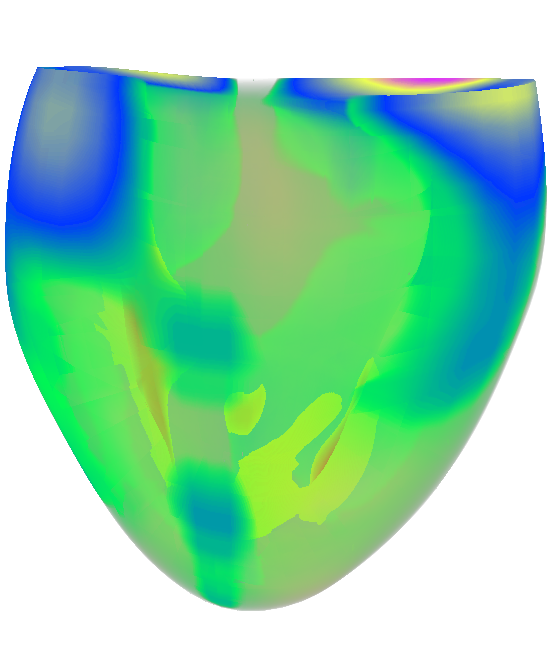
\includegraphics[width=0.99\textwidth]{figures/contributions/fem/heart-5.png}}
    \caption{Using no inter-ray or intra-ray interpolation.}
    \label{contributions:fem:raw}
\end{subfigure}
\hspace{2cm}
\begin{subfigure}[b]{0.4\textwidth}
    \fbox{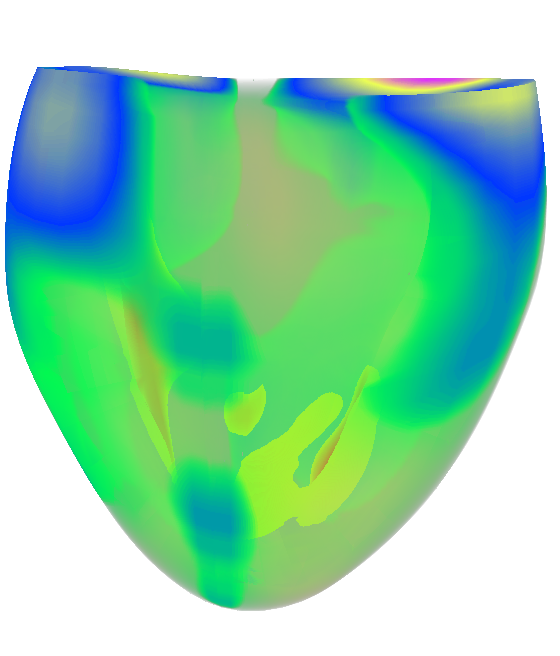
\includegraphics[width=0.99\textwidth]{figures/contributions/fem/heart-5-rr-ii.png}}
    \caption{Using inter-ray and intra-ray interpolation.}
    \label{contributions:fem:interpolation}
\end{subfigure}
\caption{A volume rendering of the heart dataset using $5\times 5$ rays per face for each element showing the difference between the interpolation schemes.}
\label{contributions:fem:interpolationexample}
\end{figure}

Lastly, we employ another technique to mitigate rendering artifacts that stem from a low sampling resolution of proxy rays.  If, for example, each face uses only a $3 \times 3$ grid of points, the same proxy ray will be used for a large area of the face; similar to nearest neighbor interpolation.  To remedy these artifacts, we effectively use bilinear interpolation on the control points of the four closest proxy rays and perform the ray marching along the spline generated by these interpolated control points.  This interpolation method is called \emph{intra-ray interpolation}.  A second interpolation method is called \emph{intra-ray interpolation}, where all rays with entry and exit points exchanged are fetched.  These are then sampled with $t' = 1-t$ and the two results are averaged before sampling the volume. \fref{contributions:fem:interpolationexample} shows the difference on the heart dataset, where $5\times 5$ rays per face for each element were generated.


% What is the domain // what is the current use // what are the current problems // what are the technical challenges // how did i meet these technical challenges // how did it work

\section{Deep Brain Stimulation Interventions} \label{contributions:dbs}
\paperef{paperB} described the work in developing a medical visualization application for deep brain stimulation~(DBS)~intervention support in collaboration with physicians at the St.~Barbara Hospital in Hamm, Germany.  This system was designed to support the brain surgeon during an electrode placement surgery in order to achieve a higher precision and thus a higher probability of a positive outcome for the patient.



\subsection{Domain and Scientific Problems} \label{contributions:dbs:background}
Deep Brain Stimulation~(DBS)~is a form of medical intervention that targets, among others, patients afflicted with Parkinson's Disease or other forms of essential tremors.  During these interventions, an electrode is inserted into patient's brain that stimulates the surrounding neurons through the use of an electric field.  Depending on the exact location of the electrode, different regions of the brain are stimulated, which has the potential to inhibit soem ofht debilitating effects of these tremors~\cite{lindberg2002impact}.  A promising target region for the treatment of tremors are the patient's subthalamic nuclei~(STN), which are two relatively small structures with the size of a few millimeters located deep in each hemisphere of the brain~\cite{benabid2009deep, richter2004determining}.  Using traditional imaging techniques such as CT or MRI, the exact location of an individual patient's STN can be difficult to determine~\cite{starr2002implantation}.  This procedure is further complicated as a small deviation in the electrodes' locations will excite other parts of the brain that can lead to undesired side-effects, such as memory loss or speech impairments.

Microelectrode Recordings~(MER)~have been developed to augment traditional imaging modalities and make use of a cluster of recording electrodes that are capable of detecting the electric activities in the brain~\cite{lenz1988methods}.  The amplitude and frequency of the electric fields measured by the electrodes correlate with specific brain regions and than hus be used to determine whether the electrodes are in the correct location~\cite{benazzouz2002intraoperative}.  The results of the MER are traditionally reviewed by the surgeon on loudspeakers in the operating room.  Aside from the obvious drawbacks of a limited auditory channel, a limited echoic memory, and potential background noise, a big challenge is the surgeon's mental separation between the spatial location of the electrodes and the results of their measurements, requiring the surgeon to keep a mental model of the brain regions and comparing those to a standard atlas in their head.  This holds true for both the absolute location of the electrode cluster as well as the relative position of the electrodes inside the cluster.

A DBS intervention is performed in three distinct phases.  In the first phase, the \emph{planning} phase, the surgeon plans the operation at his workstation by locating and segmenting the most probable location of the STN using preoperative~CT and MRI scans.  This information is used to plan an optimal access channel which evates important sensitive brain regions and selects the optimal location for the electrode to affect the~STN~\cite{butson2007patient}.  In the second phase, the \emph{recording} phase, the patient is in the operating room with their head fixed in a stereotaxic frame that restricts the patient's movement and thus allows for a fixed-body transformation and the operating room.  The MER electrode cluster is inserted into the patient's  brain along the preplanned access path until they have reached the predicted STN location.  During this phase, the measurements of the electrodes are used to discriminate the different brain regions and verify that the STN has been reached.  If the electrodes correctly identify the location of the STN, the electrodes' position along the access path is noted and their position relative to the stereotaxic frame is verified using bi-planar X-ray scans.  After this verification, the electrodes are retracted.  In the third phase, the \emph{placemenT} phase, the transmitting electrode is placed into the same location that was determined in the previous phase, which is also verified using bi-planar X-ray scans.  The exact placement and the output of the electrode is tuned using tests that examine the patient's ability, such as long term memory recall or measuring the amount of tremor.  This part of the procedure is very challenging as the patient has to be awake during the entire procedure which can last up to 10 hours.



\subsection{Application Requirements} \label{contributions:dbs:requirements}
Previous methods do not provide the surgeon with a system that sufficiently fuses the available modalities.  Preoperative CT and MRI scans, interoperative X-ray scans, the electrode measurements during the insertion, and the final patient tests are all inspected separated and the surgeon has to maintain a mental correlation between all the data sources, leading to fatigue, delays, and potential errors.  

The system described in \paperef{paperB} combines an enhanced multimodel \nD{3} volumetric rendering environment that includes





\subsubsection{System} \label{contributions:dbs:system}



% In we work package of \paperef{paperB}, the task was to develop a medical visualization application for deep brain stimulation (DBS) intervention support in collaboration with physicians at the St.~Barbara Hospital in Hamm, Germany. This system should be designed to support the brain surgeon during the surgery in order to achieve a higher precision and thus a higher probability of a positive outcome for the patient. In contrast to other medical domains, where the doctor's available preparation time for each patient is limited and thus procludes any complex interaction techniques on visualization applications, DBS interventions already have a long planning phase scheduled prior to the operation, thus enabling the usage of specialized tools and providing the ability for visualization to play an important role in this scenario.

The application resulting from this collaboration combines an enhanced multimodal \nD{3} volumetric rendering environment with the spatial visualization of electric measurements that are recording the patient's brain activity during the procedure in combination with patient-specific ability tests. Spatially embedding the measurements with the volumetric information reduces the cognitive load of the surgeon during the surgeon, as this mental link does not have to be performed by the surgeon themself. Furthermore, the system shows the uncertainties of the different modalities in a single view, thus enabling the surgeon a comprehensive view and more insight during the procedure.

\subsection{Background} \label{contributions:dbs:background}


\subsection{System} \label{contributions:dbs:system}
\begin{figure}
\fbox{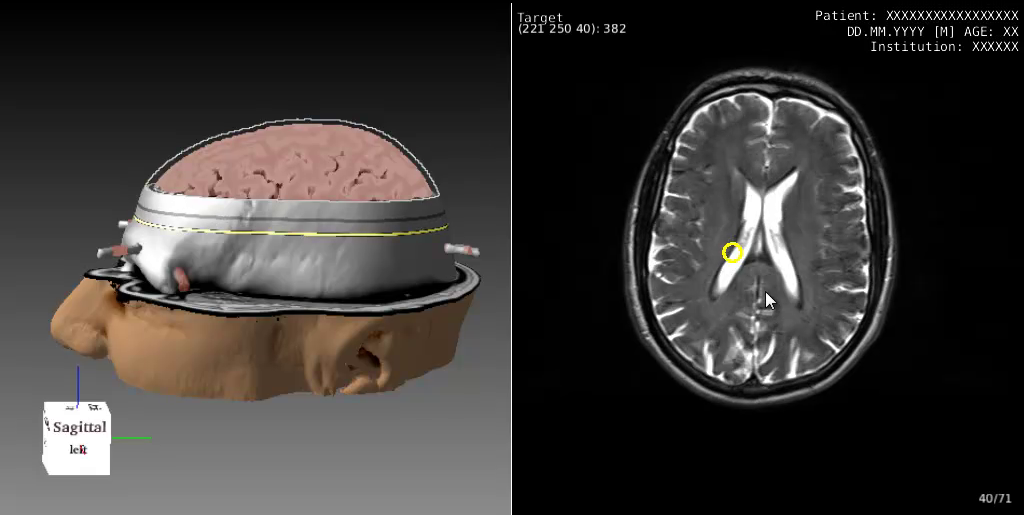
\includegraphics[width=\textwidth]{figures/contributions/dbs/planning.png}}
\caption{This view shows the part of the system that is used to import the results of a different planning tool to determine the entry point for the access path and the intented target location.}
\label{contributions:medbio:dbs:planning}
\end{figure}

In close collaboration with the surgeons, we created a system that can ingest the access path planned using other sophisticated tools (see~\fref{contributions:dbs:planning}), the various scans (T$_1$ and T$_2$ MRI, CT, and X-Ray), the MER measurements, as well as the patient tests during the operation. Combining all available modalities into one system enables the surgeon to inspect all available information for both operational phases. The system consists of multiple linked views. The \emph{Contextual view} is available in both phases, whereas the \emph{2D audio visualization} and \emph{3D audio visualization} are only available in the recording phase and the \emph{Target closeup} and \emph{Placement guide} are only available in the placement phase. The rest of this section elaborates on the design decisions for the individual views.

\question{How detailed should this be?}
\begin{figure}
\centering
\begin{subfigure}[b]{0.49\textwidth}
    \fbox{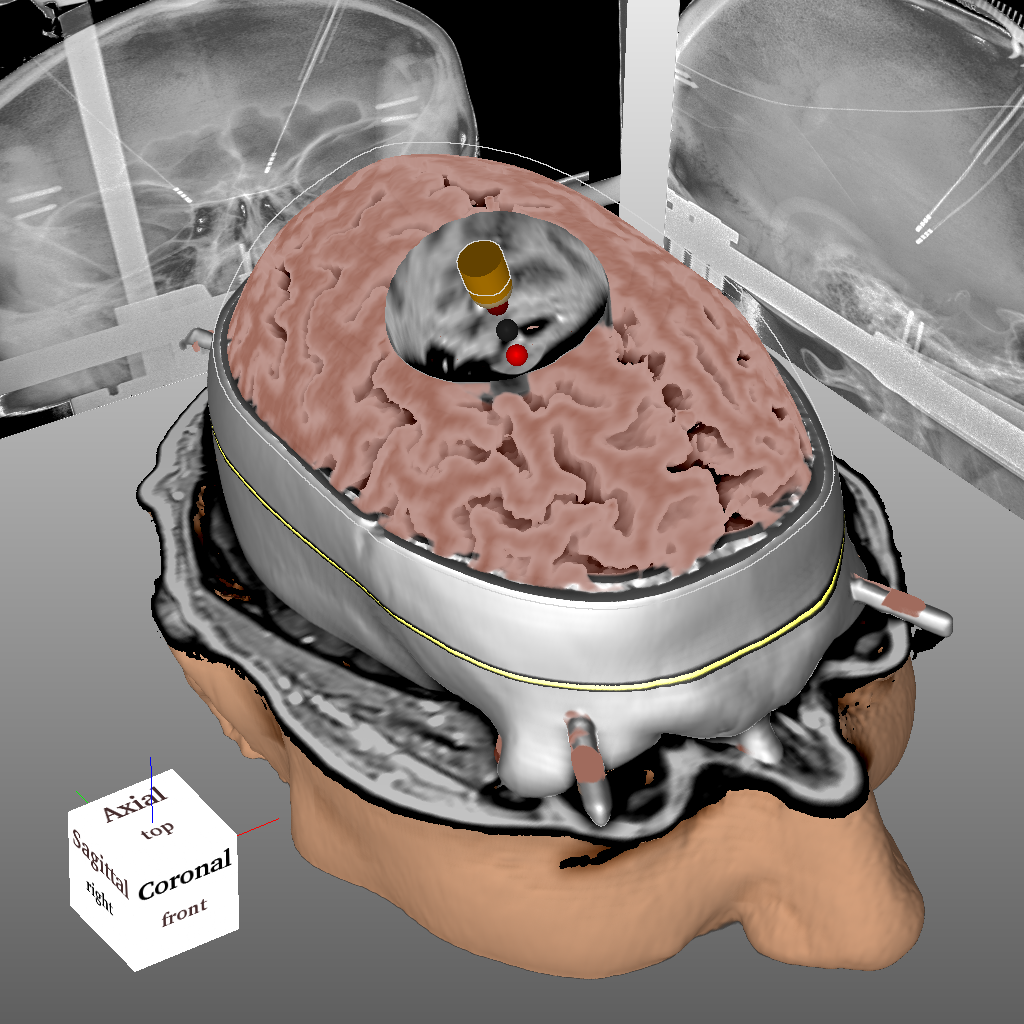
\includegraphics[width=\textwidth]{figures/contributions/dbs/recording-3d-1.png}}
\end{subfigure}
\hfill
\begin{subfigure}[b]{0.49\textwidth}
    \fbox{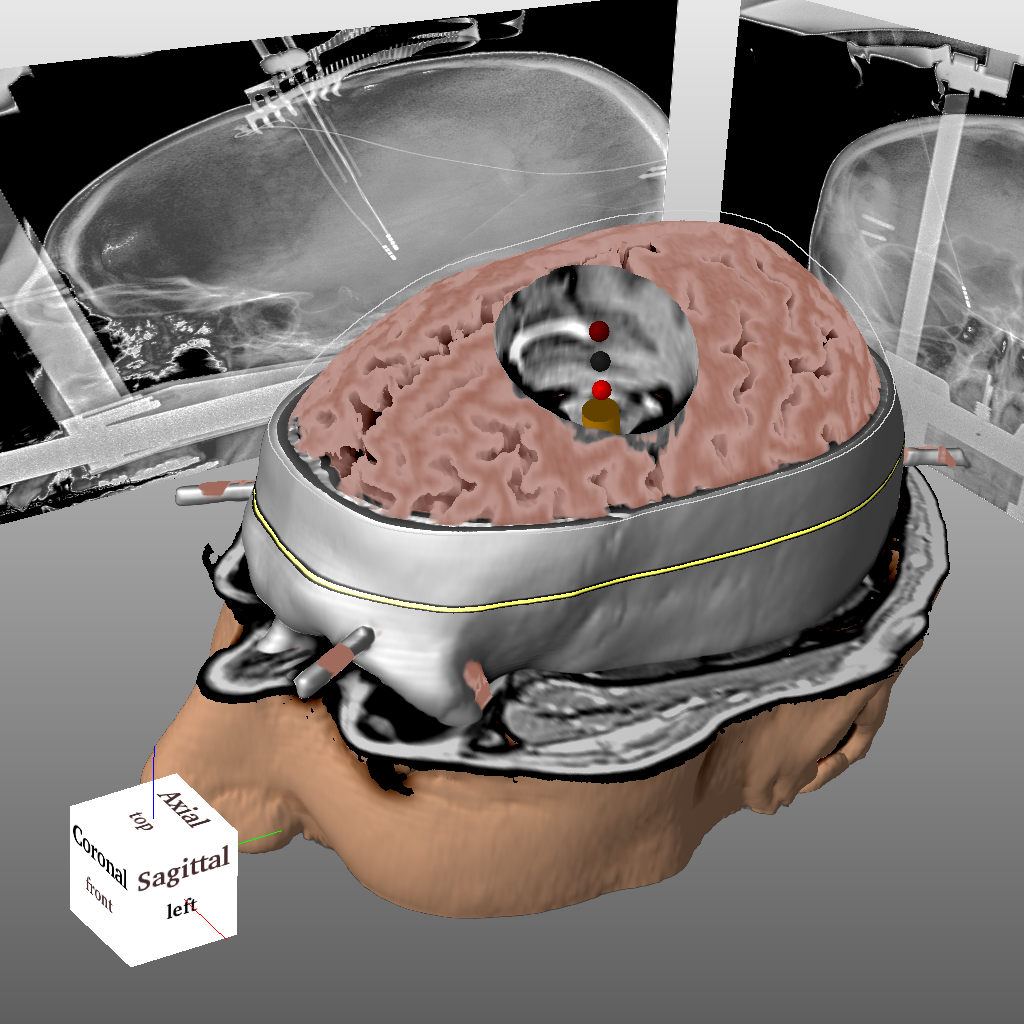
\includegraphics[width=\textwidth]{figures/contributions/dbs/recording-3d-2.png}}
\end{subfigure}
% \includegraphics[width=\textwidth]{figures/contributions/dbs/recording-3d.png}
\caption{Presenting the \emph{Contextual View} that shows the multimodal fusion of all available datasets. The preoperative CT and MRI as well as the interoperative bi-planar X-ray scans are visible together with the animated location of the electrode. The colored beads along the access path show an automatic classification of the electrode measurements.}
\label{contributions:medbio:dbs:contextual}
\end{figure}

\subsection{Contextual View} \label{contributions:dbs:contextual}
This \nD{3} view combines the preoperational CT and MRI scans together with the bi-planar X-rays and the current electrode location (see~\fref{contributions:medbio:dbs:contextual}). For improvide depth perception, we utilize a depth darkening effect as presented by Luft~\etal~\cite{luft2006image}. The selected access path is presented in this view as a carved out tunnel along which the electrode is moved during the operation. Explicitly showing the access path serves two purposes, first, it reduces the chance of a dangerous left-right mismatch error that might otherwise occur in the operation in which the electrode is accidentally inserted into the wrong hemisphere. Second, it enables us to place colored beads inside the access path behind the electrode. The colors of these beads depend on an automatic region classification of the incoming electrode signal. This method was adopted from related works~\cite{dhaese2005computer, miocinovic2007stereotactic}.

\subsection{2D audio visualization} \label{contributions:dbs:audio2d}
This view shows an augmented visualization similar to an oscilloscope that presents the direct measurements from the available electrodes. As only the amplitude and frequency are important during the procedure, we emphasize measurements that exceed a user-defined threshold and deemphasize the values below the threshold (see~\fref{contributions:medbio:dbs:sound:2d}). By this technique we highlight the potentially important measurements and reducing the visual noise from the low intensity signals. This view is linked with the \emph{3D audio visualization}, described below, such that when a specific electrode is selected in either view, it is highlighted in both views with a different color. This can be used by the surgeon to be able to correlate the detailed measurements with the relative location of the electrode.
\begin{figure}
\centering
    \begin{subfigure}[b]{0.49\textwidth}
        \fbox{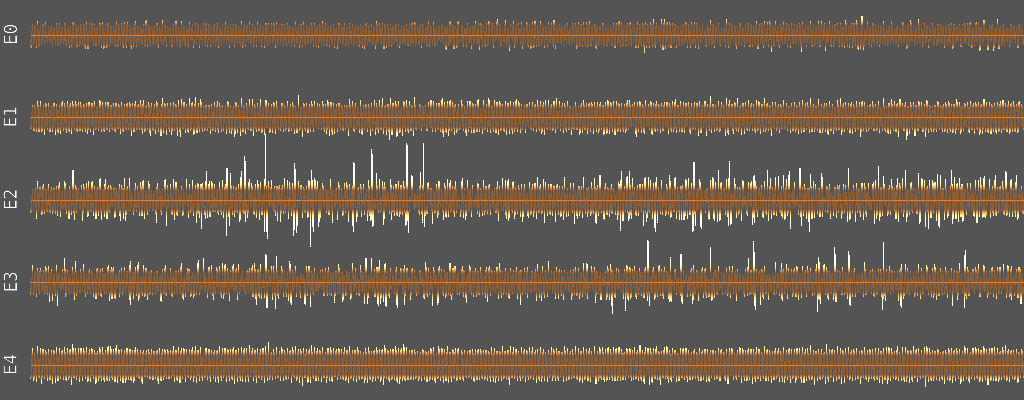
\includegraphics[width=\textwidth]{figures/contributions/dbs/audio-signal.png}}
        \caption{The \nD{2} oscilloscope rendering of the direct electrode measurements. Measurements with low amplitude are deemphasized by using darker colors.}
        \label{contributions:dbs:sound:2d}
    \end{subfigure}
    \hfill
    \begin{subfigure}[b]{0.49\textwidth}
        \fbox{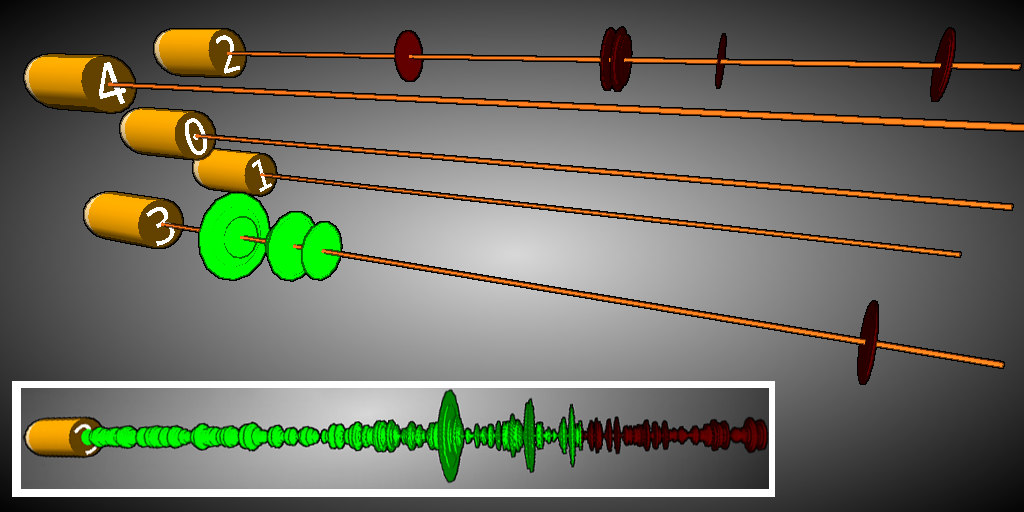
\includegraphics[width=\textwidth]{figures/contributions/dbs/recording-3dsound.png}}
        \caption{The spatial \nD{3} rendering of the electrode rendering, showing their relative spatial location and rendering the high-amplitude measurements of the signal as colored discs.}
        \label{contributions:dbs:sound:3d}
    \end{subfigure}
    \caption{This figure shows the two rendering methods for displaying the measurements recorded by the Microelectrode Recording electrodes. Both a view containing the accurate values are available (a) as well as a view showing the relative spatial relation between the electrodes.}
    \label{contributions:dbs:sound}
\end{figure}

\subsection{3D audio visualization} \label{contributions:dbs:audio3d}
In this separate view, the relative locations of the different electrodes are displayed (see~\fref{contributions:dbs:sound:3d}). The camera orientation is linked between this and the \emph{Contextual View} such that the mental registration between the two views is not broken. In this view, each electrodes' measurements that exceed a user-defined threshold are shown as discs that start at the electrode and move away from the electrode's base with increasing time. The size of the disc corresponds to the amplitude of the detected signal and thus shows the strength of the measured signal. This allows the surgeon to view the two important values (amplitude and frequency) for each of the electrodes together with their spatial orientation. The color of each disc is determined by the same classification algorithm that is used on the beads in the \emph{Contextual View}, but is simplified to show red if the electrode is outside of the STN and green if it is inside the STN. The surgeon can then, by correlating the frequency of discs and their amplitude verify that the classification was correct and that the electrodes are in the correct location.

\begin{figure}
\fbox{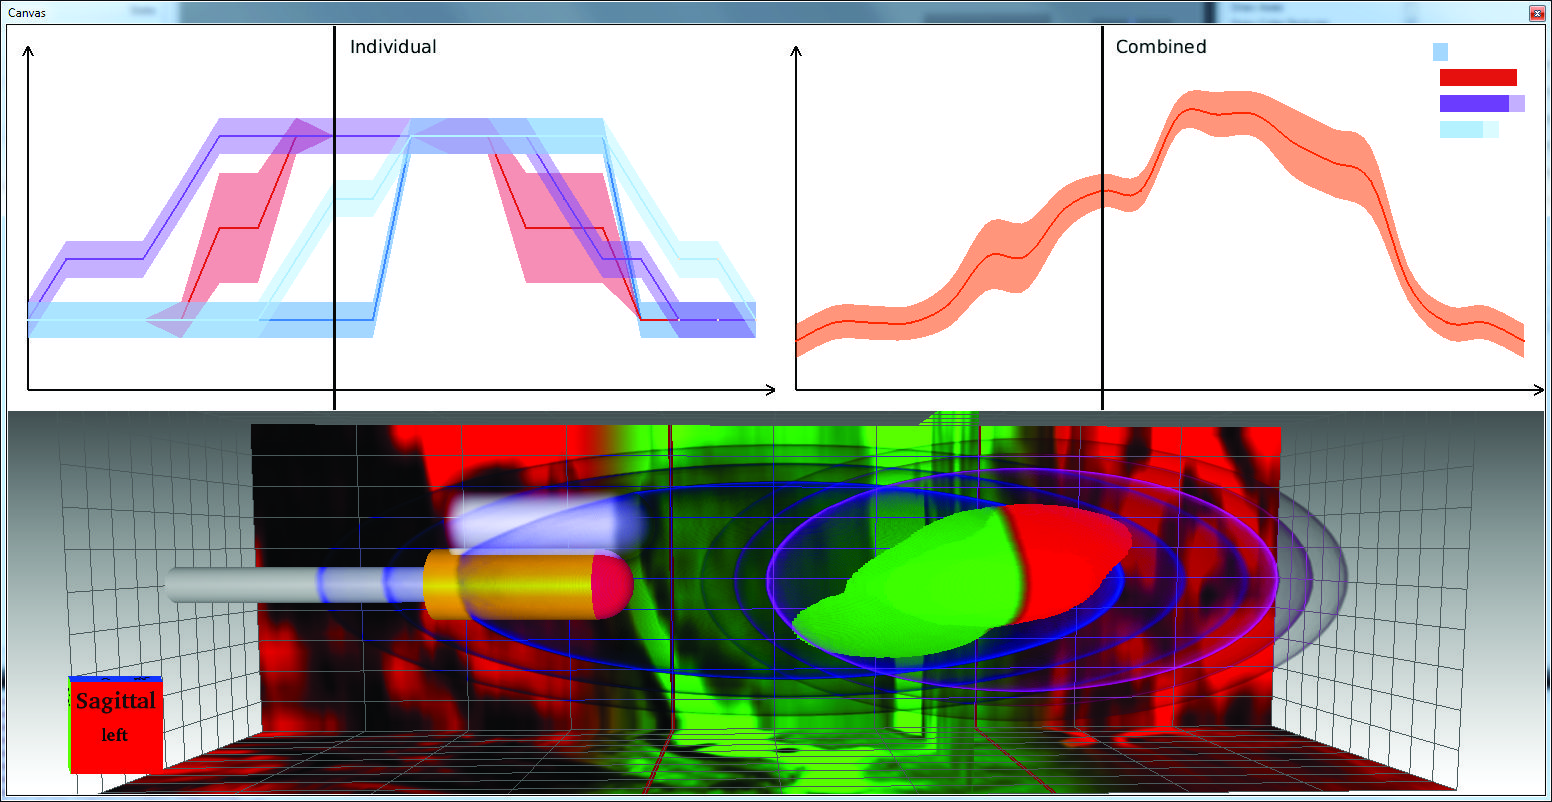
\includegraphics[width=\textwidth]{figures/contributions/dbs/screenshot-target.jpg}}
\caption{The views that show the results of the different measurements performed during the recording phase. The \emph{Target closeup} (bottom view) contains the segmented location of the STN is visible as well as the results of the different tests at their spatial location. The \emph{Placement guide} shows the likelihood measurements according to their depth along the access path}
\label{contributions:dbs:target}
\end{figure}

\subsection{Target closeup} \label{contributions:dbs:target}
After the potential electrode location has been determined, the surgeon uses this closeup view, centered around the segmented location of the STN, that combines all of the information that was gathered in the recording phase (see~\fref{contributions:dbs:target} bottom). Embedded in this view are the locations of the electrode as determined by the depth along the access path together with their reconstructed location using the biplanar X-ray scans. In addition it shows the MER signal results as a red-green overlay on the backside of the bounding box and presents options to add patient test results as additional half-transparent oval overlays. As all of these values have their own, unknown, uncertainty this view displays the overlap of the regions to inform the surgeon of a potential final placement that agrees with most measurements. On demand, the surgeon can enable the rendering of the MRI scan around the STN.

\subsection{Placement guide} \label{contributions:dbs:placement}
This view is based on the same information as the \emph{Target closeup}, but presents the information in a line plot, whose ordinate shows the likelyhood of a correct placement for each measurement and the abcissa shows the depth along the access path (see~\fref{contributions:dbs:target} top). We display an estimate of uncertainty for each value by extruding the line with a transparent band.

\subsection{Evaluation} \label{contributions:dbs:evaluation}
In order to perform an initial evaluation of the system, we conducted a qualitative user study with five neurosurgeons, which all had experience with conducing DBS interventions. Each of the participants watched the usage of the system during the planning, recording, and placement phase. The data for this test case was recording during an operation performed by one of the coauthors. Then, each participant answered a questionnaire that used eight of the questions suggested by Martelli~\etal for evaluating computer-aided surgery systems~\cite{martelli2003criteria} with an additional free form text field for comments.

% \subsection{Generalizability} \label{contributions:dbs:generalizability}
% As mentioned in \charef{visapp}, one opportunity for application papers to advance the field of visualization is by providing generalizable solutions. To this end, the entire system was implemented in the Voreen framework~\cite{meyer2009voreen}, which allows the reusability of individual components. Judging the work package from this point of view, there are two parts that can provide useful in other application domains.

% \subsubsection{Audio Visualization} The 3D audio visualization that is used to display the MER measurements in a spatial context can be extended to any kind of timevarying data that can be filtered by a binary filter and where the spatial location of the individual measurements is important.

% \subsubsection{Uncertainty Ranges} The visualization of the uncertainty ranges in the \emph{Target closeup} view might also prove beneficial to other domain areas in which multiple uncertain sources are used to pinpoint a most likely location of a target region. Naturally, they do not have to be isotropic uncertainties, but any form of visual feedback between spatial locations and uncertainties can be useful.






\section{Urban Search \& Rescue} \label{contributions:usar}
Papers~\ref{pa:paperC}, \ref{pa:paperD}, and \ref{pa:paperE} were developed in the domain or \emph{Urban Search \& Rescue}, a field of civil security that involves the location and possible extraction of victims that are trapped in a partially or fully collapsed building.  The goal was to design an application in collaboration with the Myndigheten f\"or samh\"allsskydd och beredskap, the Swedish Civil Contingencies Agency, that expedites the location of vicims in buildings through the use of sensor-equipped autonomous drones.


% What is the domain // what is the current use // what are the current problems // what are the technical challenges // how did i meet these technical challenges // how did it work

\subsection{Domain and Scientific Problems} \label{contributions:usar:background}
\begin{wrapfigure}{o}{0.4\textwidth}
\centering
\fbox{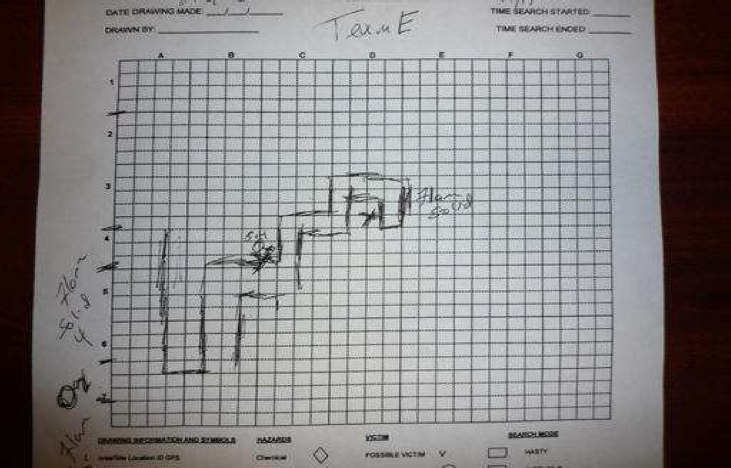
\includegraphics[width=0.38\textwidth]{figures/contributions/usar/map_drawing.jpg}}
\caption{A hand drawn map showing the state-of-the-art method for coordinating multiple rescuers.}
\label{contributions:usar:map:hand}
\end{wrapfigure}

Traditionally, in the case of a partial building collapse in an urban environment, the countries' civil contingencies agencies will perform an urban search \& rescue operation in order to search the building for potentially injured survivors or victims and perform an extraction.  This method entails \emph{responders} to enter the building being directed and coordinated by an \emph{incident commander}~(IC).  The major obstacle during these rescue operations involving partially collapsed buildings is the fact that previous structural plans are no longer usable and new hazardous environments may have been created in the incident.  In addition, the viewing distance is usually restricted as debris and smoke impede the responders.  During the rescue operation, the IC relies on the descriptions of the responders to manually create a map~(see \fref{contributions:usar:map}).  This map is important for the IC in order to 1. optimally coordinate the available rescuers as time-to-rescue is the dominating factor in determining a victim's survivability and 2. due to the collapses in the buiding, entire parts of the building might be inaccessible without removing rubble.  These \emph{voids} are prime locations of trapped victims and their detection on a \nD{2} map of a complex \nD{3} structure is difficult.

\begin{wrapfigure}{o}{0.4\textwidth}
\centering
\fbox{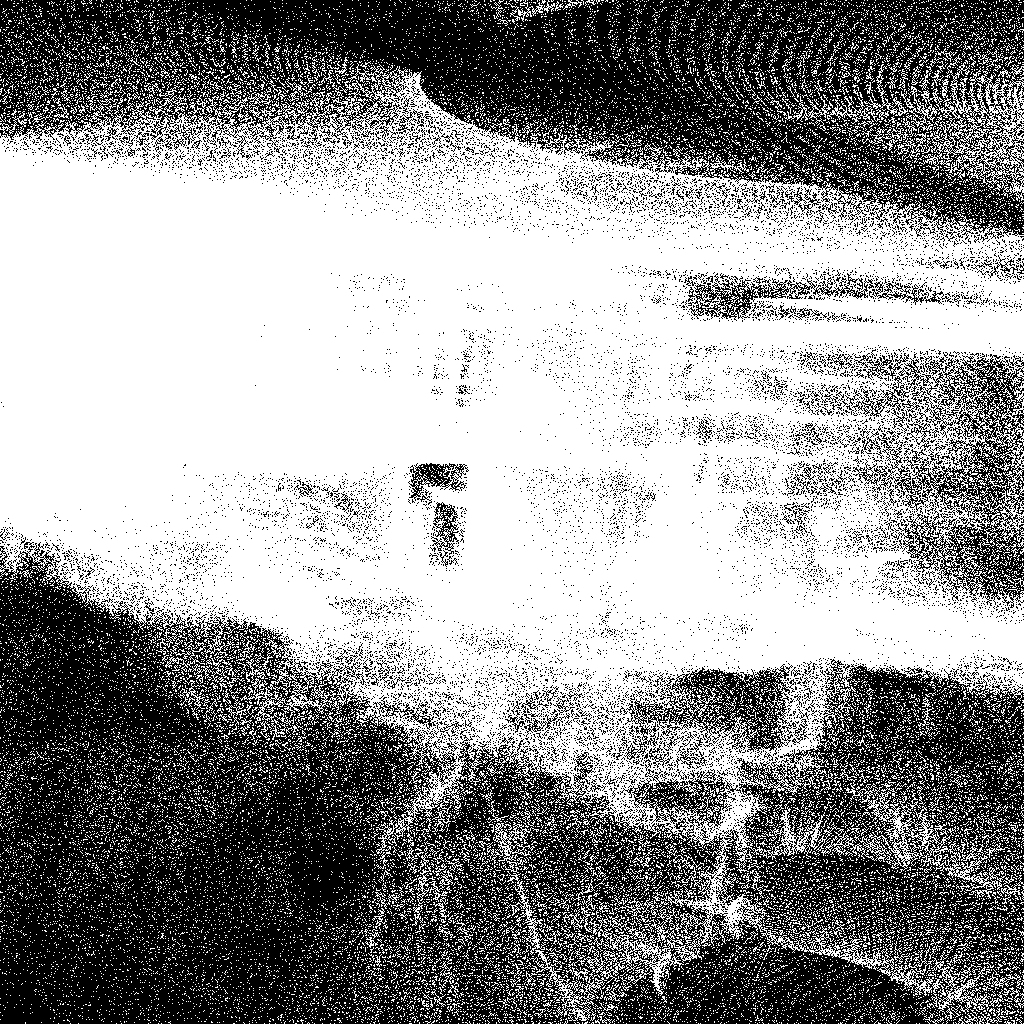
\includegraphics[width=0.38\textwidth]{figures/contributions/usar/map_pointcloud.jpg}}
\caption{A naive rendering of the point cloud makes it difficult to inspect details in the building.}
\label{contributions:usar:map:pointcloud}
\end{wrapfigure}

The robotics community, for a long time, has been advancing research into sensor-equipped drones and autonomous control in the usage for urban search \& rescue~\cite{liu2013robotic}, which makes it feasible to improve the current workflow and create a system supporting the IC during a rescue operation.  While traversing the building, the rescue robots carry a variety of scanners, for example LiDAR, heartbeat detectors, or scanners to detect gas leaks.  These scans are then combined to create a complete \nD{3} point cloud map of the entire structure that the IC can use to plan a more efficient  advancement of available responders.  The maps in their native form (see \fref{contributions:usar:map:pointcloud}), however, are difficult to interpret due to the lack of occlusion and other visual queues.  Furthermore, important aspect of the map for determining a path for responder, such as location and dangerous environments, the slope of terrain, the existence of overhangs and the available space for a responder's body are diffcult to extract in the maps current state.  Therefore, papers~\ref{pa:paperC}, \ref{pa:paperD}, and \ref{pa:paperE} set out to make the inspection and analysis of the \nD{3} point cloud data easier for the IC and suggest a variety of paths in order to move the current ad-hoc decision make into a superior planning mode.  As the data is likely to be noisy and the domain knowledge of the IC is important in the decision making, a fully automatic algorithm is not desireable, but rather to generate a set of suggestions and the visualization tools enabling the IC to make a good selection out of a set of suggestions.


\subsection{Application Requirements} \label{contributions:usar:requirements}
\begin{figure}
\centering
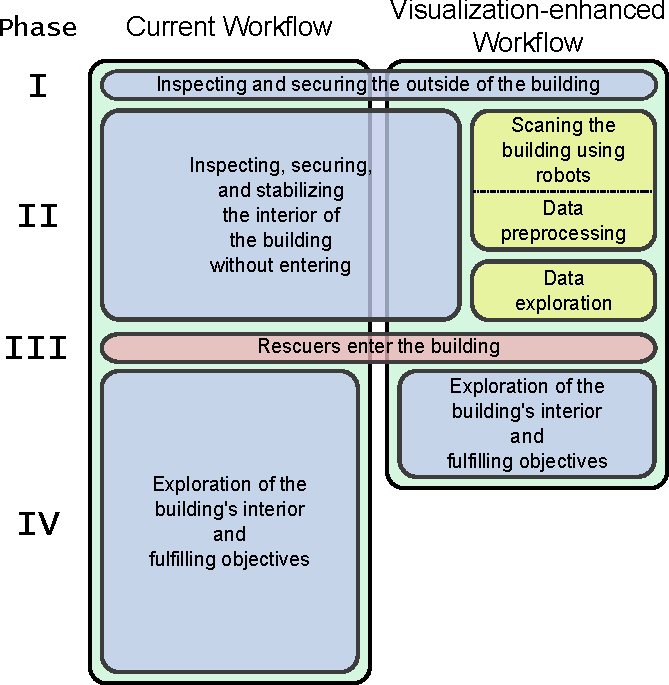
\includegraphics[width=0.75\textwidth]{figures/contributions/usar/workflow.pdf}
\caption{Analyzing the currently employed workflor of the rescue operation, it is possible to retrieve full scans of the building during the initial inspection phase during which no human is allowed into the building.  The gathered information can then later decrease the time necessary to explore the building.}
\label{contributions:usar:workflow}
\end{figure}

Papers~\ref{pa:paperC}, \ref{pa:paperD}, and \ref{pa:paperE} describe the effort of developing a system that provides the IC with the tools to analyze the aquired point cloud data and that suggests a set of paths together with the visualization tools to analyze the paths and make an informed decision about a path selection.  The system thus needs to meet a set of challenges in order to be beneficial to the IC; 1. The system must increase spatial awareness and depth perception by allowing for interactive exploration of the collapsed structure.  2. The system must enable the IC to interactively annotate the acquired data to react to changing circumstances.  These annotations are potential entry points, points of interest (POI), and the ability to add and remove obstacles from the map, as all of these can and will change during the course of a rescue operation.  3. The system must automatically generate a set of candidate paths for the responders and provide the IC with the tools to inspect the available access paths, compare them, make trade-offs, and select and execute the optimal path.  The different paths are generated by changing importance weights on the path computation algorithm which leads to a set of distinct paths that cover a multi-dimensional decision space and includes paths that favor, for example, a more dangerous path over a shorter path.  These paths are then presented to the IC together with decision-making tools in order to select the single path that is then executed.


\subsection{Voxel Binning} \label{contributions:usar:binning}
\begin{figure}
\centering
\begin{subfigure}[b]{0.28\textwidth}
    \fbox{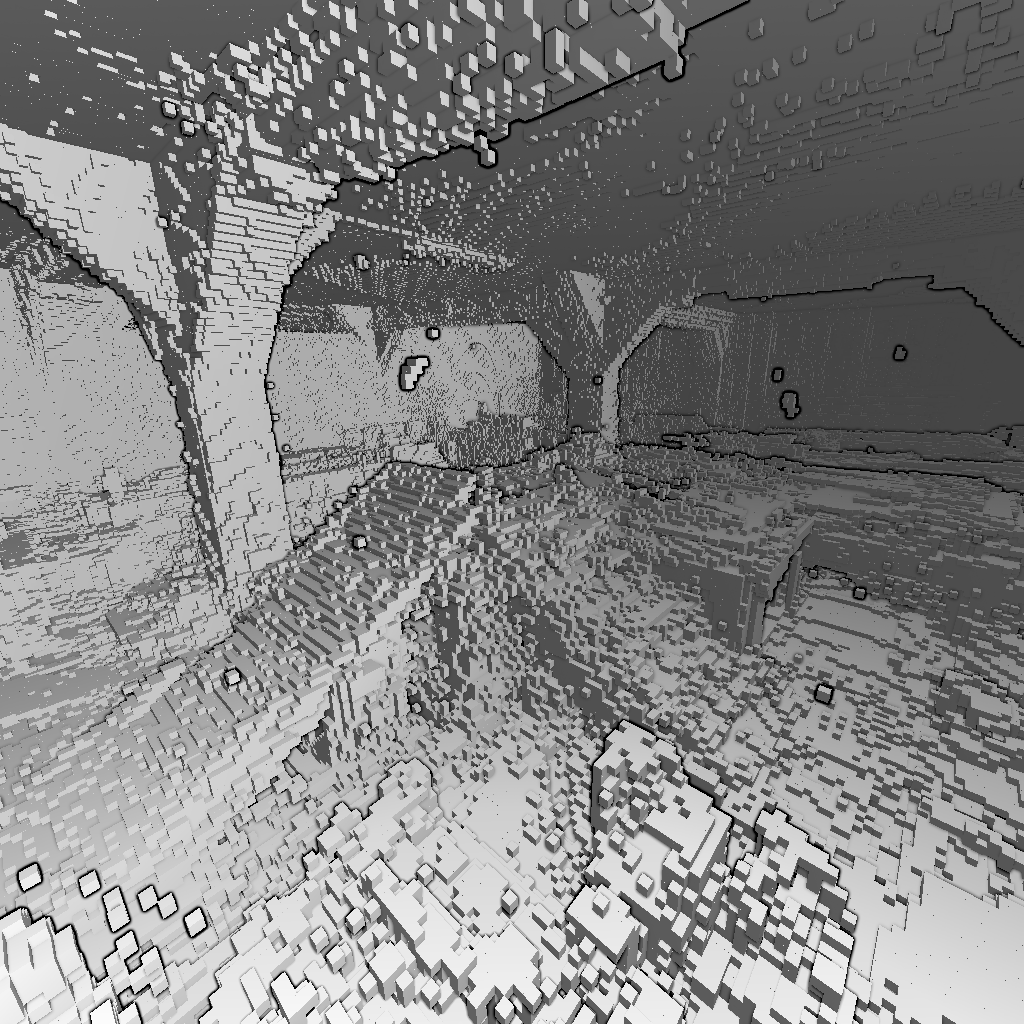
\includegraphics[width=0.99\textwidth]{figures/contributions/usar/bin_4.png}}
    \caption{Binning of a dataset with a voxel size of 4\,cm.}
    \label{contributions:usar:binning:4}
\end{subfigure}
\hspace*{5mm}
\begin{subfigure}[b]{0.28\textwidth}
    \fbox{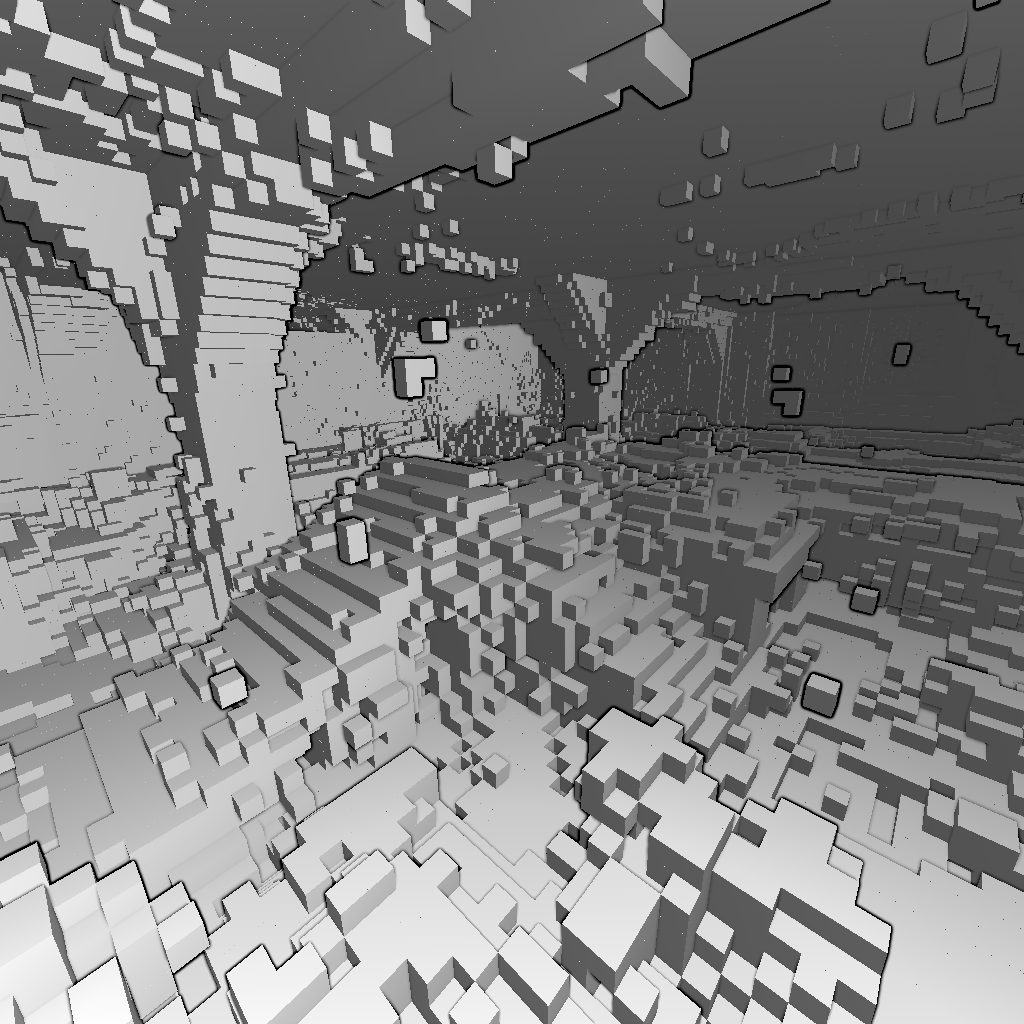
\includegraphics[width=0.99\textwidth]{figures/contributions/usar/bin_10.png}}
    \caption{Binning of a dataset with a voxel size of 10\,cm.}
    \label{contributions:usar:binning:10}
\end{subfigure}
\hspace*{5mm}
\begin{subfigure}[b]{0.28\textwidth}
    \fbox{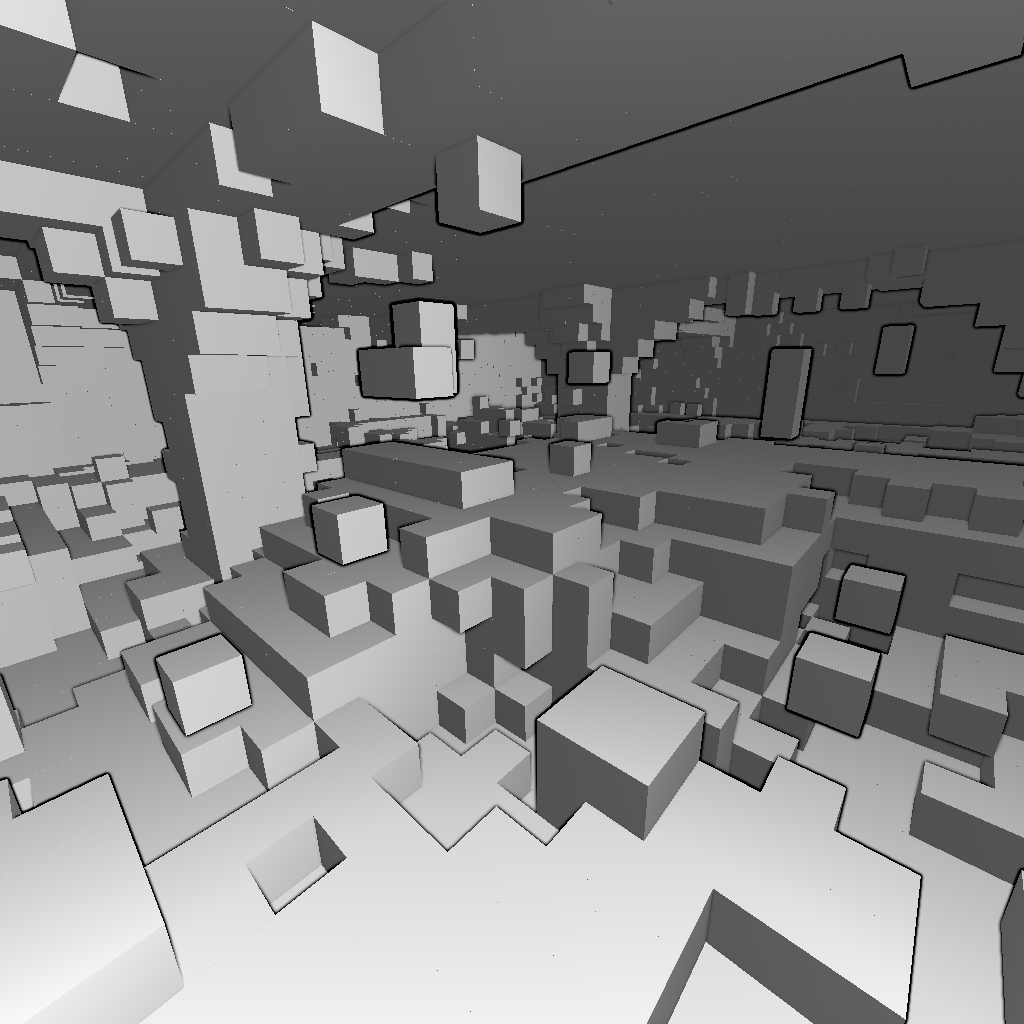
\includegraphics[width=0.99\textwidth]{figures/contributions/usar/bin_25.png}}
    \caption{Binning of a dataset with a voxel size of 25\,cm.}
    \label{contributions:usar:binning:25}
\end{subfigure}
\caption{The resolution of the voxel grid has a direct impact on the trade-off between achieved resolution and the amount of sensor noise that is included in the data.  Here, a rescue arena from the Jacobs University rescue arena is used.}
\label{contributions:usar:binning}
\end{figure}

The combined map as retrieved from the unmanned drones is an unstructured point cloud (see \fref{contributions:usar:map:pointcloud}) and does not allow for easy interpretation as the individual points are not space filling and thus provide no depth clues to the user.  In order to solve this challenge and provide the user with a familiar view of the building's interior, a binning technique is applied to the point cloud.  For a user-defined binning size, a voxel grid is created that covers the extend of the point cloud.  Each voxel in the grid is marked with the number of points which fall into its extend and only voxels with an \emph{occupancy} of greater than a fixed value are considered.  \fref{contributions:usar:binning} shows an example of the same point cloud binned with voxels of different bin sizes.  The size of the voxels depends on the resolution of the scanner that is employed where a larger bin size deemphasizes the noise in the data and a smaller bin size provides higher detail.  For the binning, we use the widely utilized point cloud library PCL that provides efficient methods to construct out-of-core voxel grids as well as reconstruct surfaces from the data~\cite{rusu20113d}.  These grids are then converted into a new point cloud, where only the center point of each voxel is stored.

In addition to the LiDAR data that is used to determined whether individual voxels are present in the map, additional scanners or manual input can be used to mark voxels.  These markings can be the location of potential entry points into the structure, the location of victims or other points of interests, or the location, type, and severity of hazardous environments.  Based of this information, it is possible to compute other, derived attributes, for the voxels in the grid.

\begin{description}[leftmargin=6em,style=nextline]
  \item[Hazard]    The distance to the closest voxel that is marked with as a hazardous environment.
  \item[Support]   The number of unobstructed surrounding voxels at the same height, given a desired floor support for a human responder of about $40\times40\,$cm.
  \item[Size]      The amount of space that is available above the specific voxel indicating whether it is necessary for the responder to walk or crouch over this location.
  \item[Normal]    Determines the orientation of the original point cloud that this voxel covers based on a reconstructed surface model.  If the normal strongly deviates from the gravity vector, the more dangerous it is for responder to traverse.
  \item[Occupancy] The amount of points in the original point cloud that are covered by the voxel.  This provides an indication of the certainty that the voxel is not a scanning artifact.
  \item[Overhang]  Determines whether there is an overhang, which is a potentially unstable structural element above the voxel.
\end{description}

All computed values are stored for each occupied voxels and most are utilized in the path computation to favor or exlude certain areas of the map.  By varying the weight of each value, it thus becomes possible to generate a set of paths that are each optimal for the specific weight values but provide the IC with a set of candidate paths from which to choose.


\subsection{Path Computation} \label{contributions:usar:binning}
In order to perform the path computation, the system uses the widely used \astar algorithm which utilizes a \emph{metric} or \emph{cost function} $\textrm{m}(\mathbf{x_1}, \mathbf{x_2})$ to determine the cost or error to move between two nodes $\mathbf{x_1}$ and $\mathbf{x_2}$ in a graph~\cite{hart1968formal} and a heuristic $\textrm{h}(x_1)$ to determine the approximate the remaining distance to the goal.  \astar is an \emph{informed} algorithm that, for a given graph and metric, finds the optimal path between two points through an exhaustive greedy search of the graph.  In the case of the voxel grid, each voxel is treated as a node with a theoretical maximum of 26 edges, if all of surrounding voxels are filled.  The interested reader is referred to the book by Russel and Norvig for a full description of the \astar algorithm~\cite{russell1995modern}.  

The only requirement for the heuristic, $\textrm{h}(\mathbf{x_1})$, is that it is \emph{admissable}, which means that it never overestimates the distance between $\mathbf{x_1}$ and the goal.  For the path computation in the voxel grid, the $L^2$-norm is used as an heuristic.  It is admissable as the movement along the voxels follows the $L^1$-norm and is thus guaranteed to be larger than $\textrm{h}(\mathbf{x_1}) \; \forall \mathbf{x}$.

\textbf{Cost function.}  The design of the cost function $\textrm{m}(\mathbf{x_1}, \mathbf{x_2})$ is of vital importance for the \astar algorithm as it defines the resulting path's optimality.  This system uses a cost function that consists of a number of additive, weighted sub-functions.  Thus, the optimal path will be different for each combination of weighting factors.  This enables us to construct a multi-dimensional search space $\mathcal{P}$ with each element $\mathbf{w} \in \mathcal{P}$ being a set of weights and parameters and thus associated with a single optimal path through the voxel grid.  In the current system, $\mathcal{P} = \mathbb{R}^8$ with parameters for the hazard $w_h$, size $w_s$, normal $w_n$, normal threshold $\varphi$, support $w_{sup}$, desired support $n$, overhead $w_o$, and occupancy $w_{occ}$, although it is trivial to include the dimensionality of the search space, which drastically increases the computation times (see below).

Thus the final cost function is defined as:
\begin{equation}
\begin{array}{r@{}l}
m(\mathbf{x_1}, \mathbf{x_2}) = & L_2(\mathbf{x_1},\mathbf{x_2}) + w_h \cdot \textrm{hazard}(\mathbf{x_2}) + w_s \cdot \textrm{size}(\mathbf{x_2}) + \vspace*{0.1cm} \\
  & w_n \cdot \textrm{normal}(\mathbf{x_2}, \varphi) + w_{sup} \cdot \textrm{support}(\mathbf{x_2}, n) + \\
  & w_o \cdot \textrm{overhead}(\mathbf{x_2}) + w_{occ} \cdot \textrm{occupancy}(\mathbf{x_2})
\end{array}
\end{equation}

\textbf{Path classes.}  When sampling $\mathcal{P}$ sufficiently high with about $10^7-10^9$ samples, it became clear that many of the sampled weights resulted in only a small number of representative paths with only minor or no variation.  We therefore grouped the computed paths into classes by comparing the ordered list of voxels that uniquely defines a path.  For a user-defined threshold $a$, paths are considered equal if at most $a$ subsequent voxels in the ordered list are different.  This reduces the number of paths that need to be considered during the rendering drastically and thus increases performance and legibility of the visualizations.

\begin{figure}
\centering
\begin{subfigure}[b]{0.4\textwidth}
    \fbox{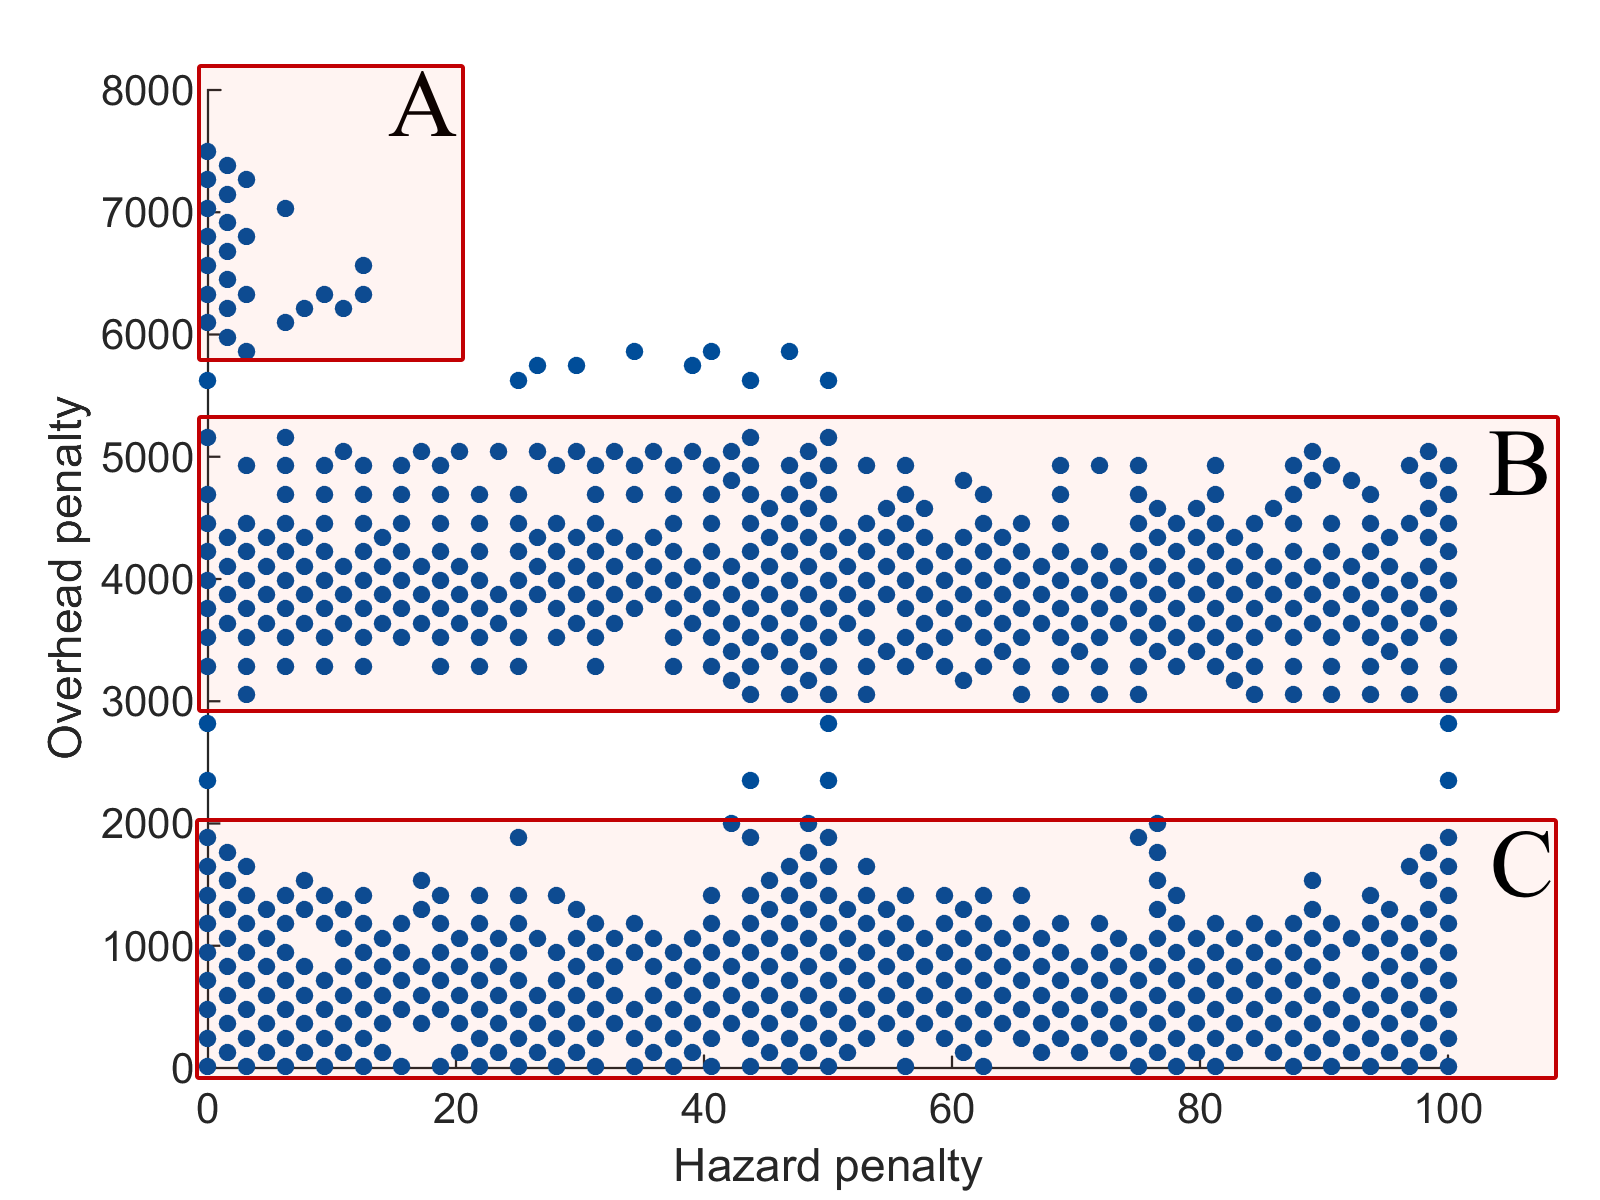
\includegraphics[height=4.5cm, width=0.99\textwidth]{figures/contributions/usar/adaptive_sampling_space.png}}
    \caption{The hazard-overhead subspace of the parameter search space $\mathcal{P}$ shows three path classes.}
    \label{contributions:usar:adaptive:space}
\end{subfigure}
\hspace*{1cm}
\begin{subfigure}[b]{0.3\textwidth}
    \fbox{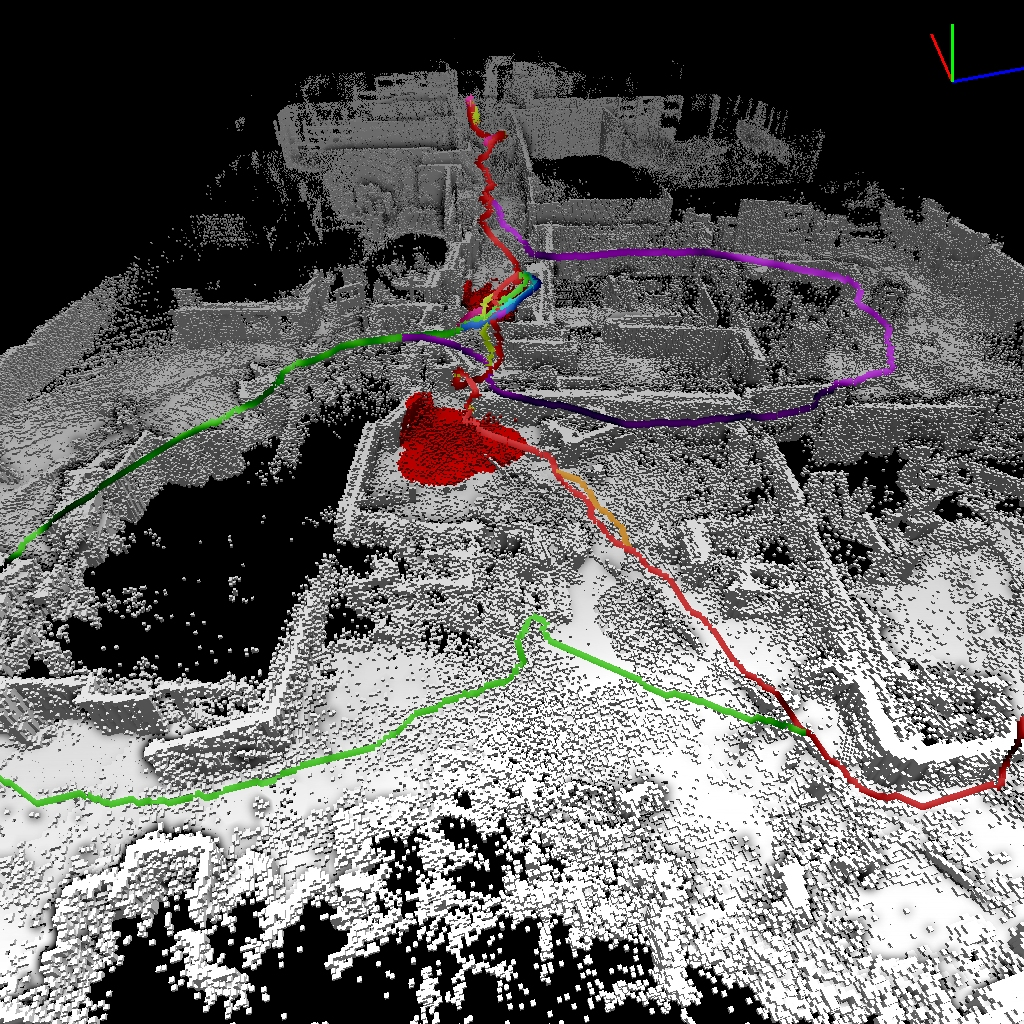
\includegraphics[height=4.5cm, width=0.99\textwidth]{figures/contributions/usar/adaptive_sampling_rendering.jpg}}
    \caption{The three path classes clearly show up as distinct when inspected.}
    \label{contributions:usar:adaptive:rendering}
\end{subfigure}
\caption{During the adaptive sampling, it was found that paths cluster in the multi-dimensional space, which correspond to individual path clusters.}
\label{contributions:usar:adaptive}
\end{figure}

\textbf{Adaptive sampling.}  As there is no prior information available about $\mathcal{P}$, providing a reasonable sampling strategy is not trivial.  A regular grid sampling is insufficient as plausible boundary values for each dimension are not known, thus incurring the risk of over- or undersampling the path space.  In order to search $\mathcal{P}$ more efficiently, the system utilizes a binary space partitioning such that new samples are only generated in those regions of $\mathcal{P}$ that have the potential of providing a new class of path.  Previously computed paths devide the space $\mathcal{P}$ such that new samples are only created where there is the potential of resulting in new paths.  This assumes that if samples $\textbf{p}$ and $\textbf{q} > \textbf{p}$ result in the same path

Using the previously computed paths the space $\mathcal{P}$ is divided such that new samples of $\mathcal{P}$ are only created where there is the potential of generating novel paths.  All potential samples are classified into either non-recursive or recursive samples.  In each interation, each dimension is bisected and the each recursive sample is tested against the neighboring samples to determine whether a region should be subdivided.  The subdivision will continue until all recursive samples return non-novel paths or until the distance between samples is smaller than a predefined threshold $\epsilon$.  This threshold is necessary as the subdivision would otherwise converge to the boundary and result in an arbitrary large number of samples.   This method only requires the specification of arbitrary initial bounds for the weights and the adaptive sampling method will only perform new computations where necessary.  \fref{contributions:usar:adaptive} shows the subspace of hazard-overhead penalty and shows the three groups of paths that are present when visually inspecting the data.



\subsection{Rendering} \label{constributions:user:rendering}
\begin{figure}
\centering
\begin{subfigure}[b]{0.21\textwidth}
    \fbox{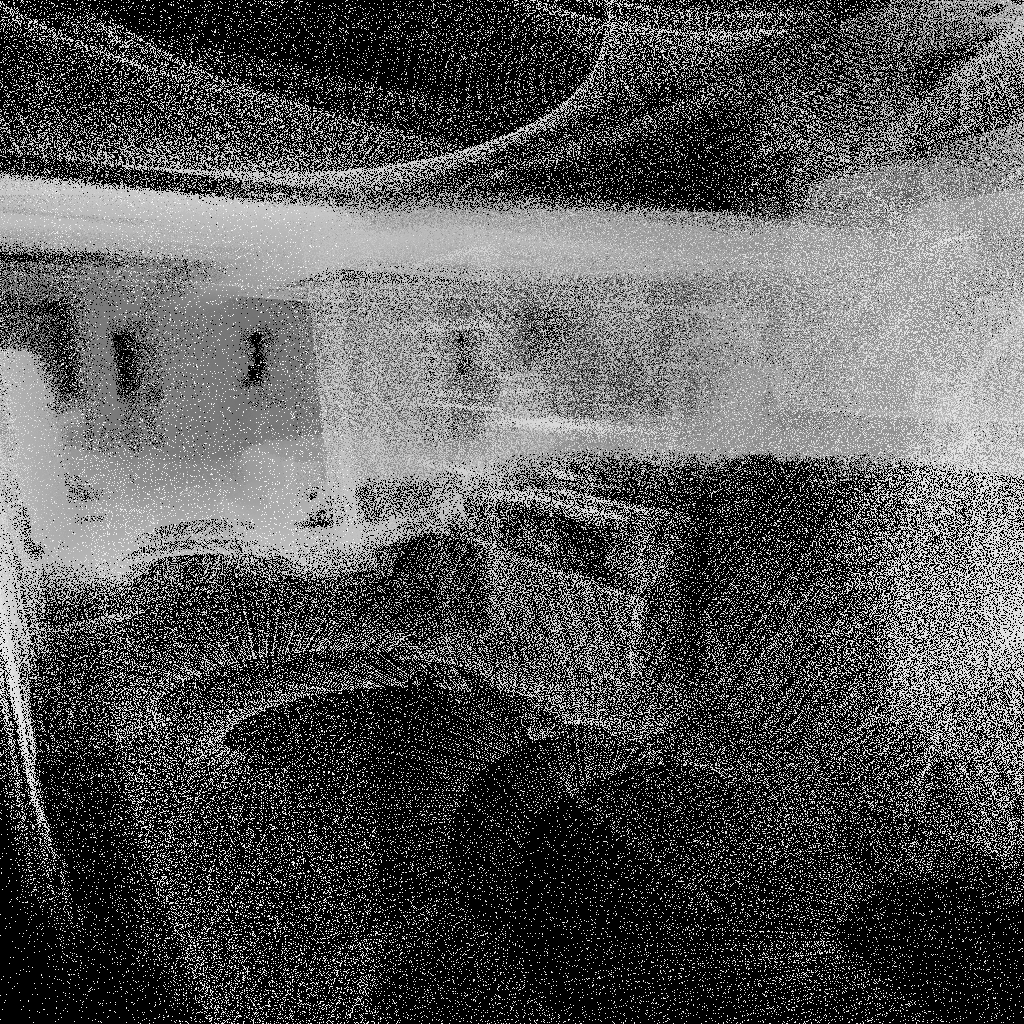
\includegraphics[width=0.99\textwidth]{figures/contributions/usar/rendering_points.png}}
    \caption{Rendering of the unstructured, unbinned point cloud.}
    \label{contributions:usar:rendering:points}
\end{subfigure}
\hspace*{2.5mm}
\begin{subfigure}[b]{0.21\textwidth}
    \fbox{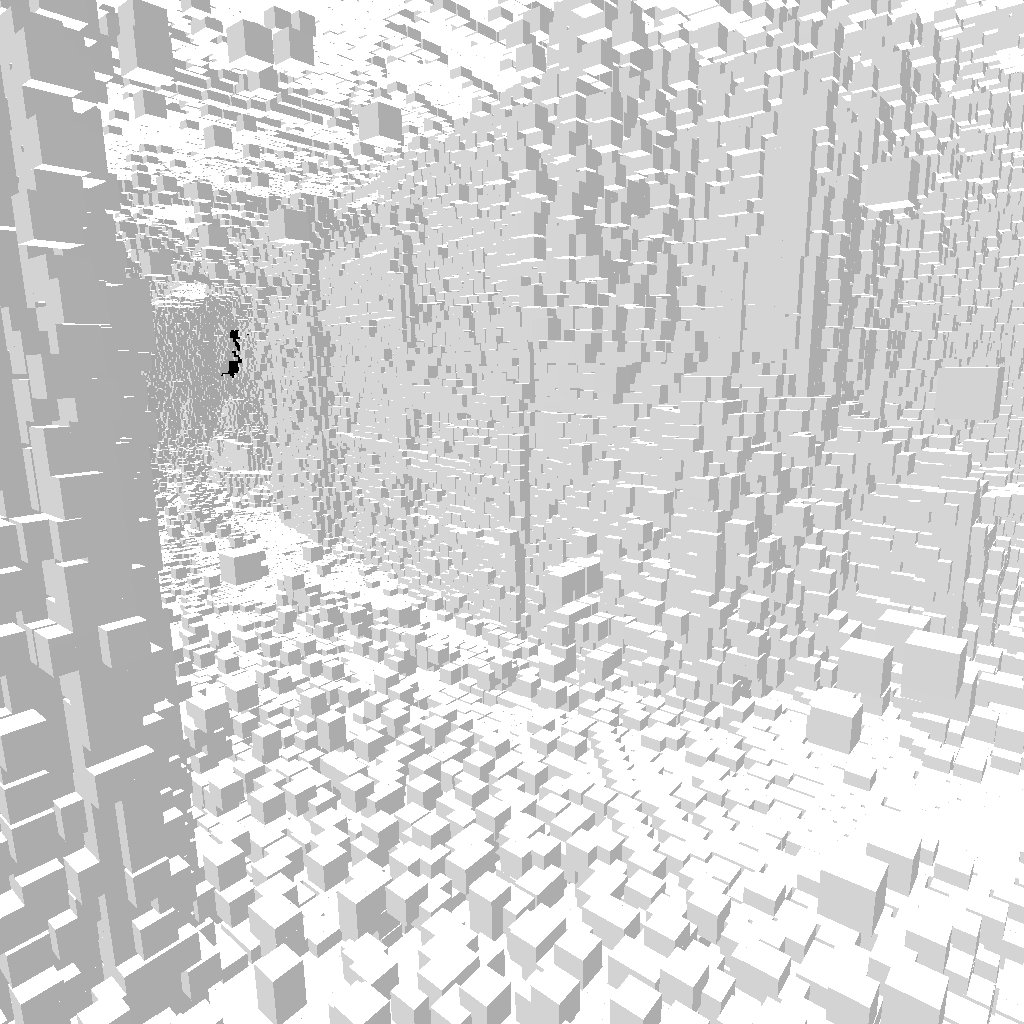
\includegraphics[width=0.99\textwidth]{figures/contributions/usar/rendering_default.png}}
    \caption{Rendering of the axis-aligned boxes using only Phong shading.}
    \label{contributions:usar:rendering:default}
\end{subfigure}
\hspace*{2.5mm}
\begin{subfigure}[b]{0.21\textwidth}
    \fbox{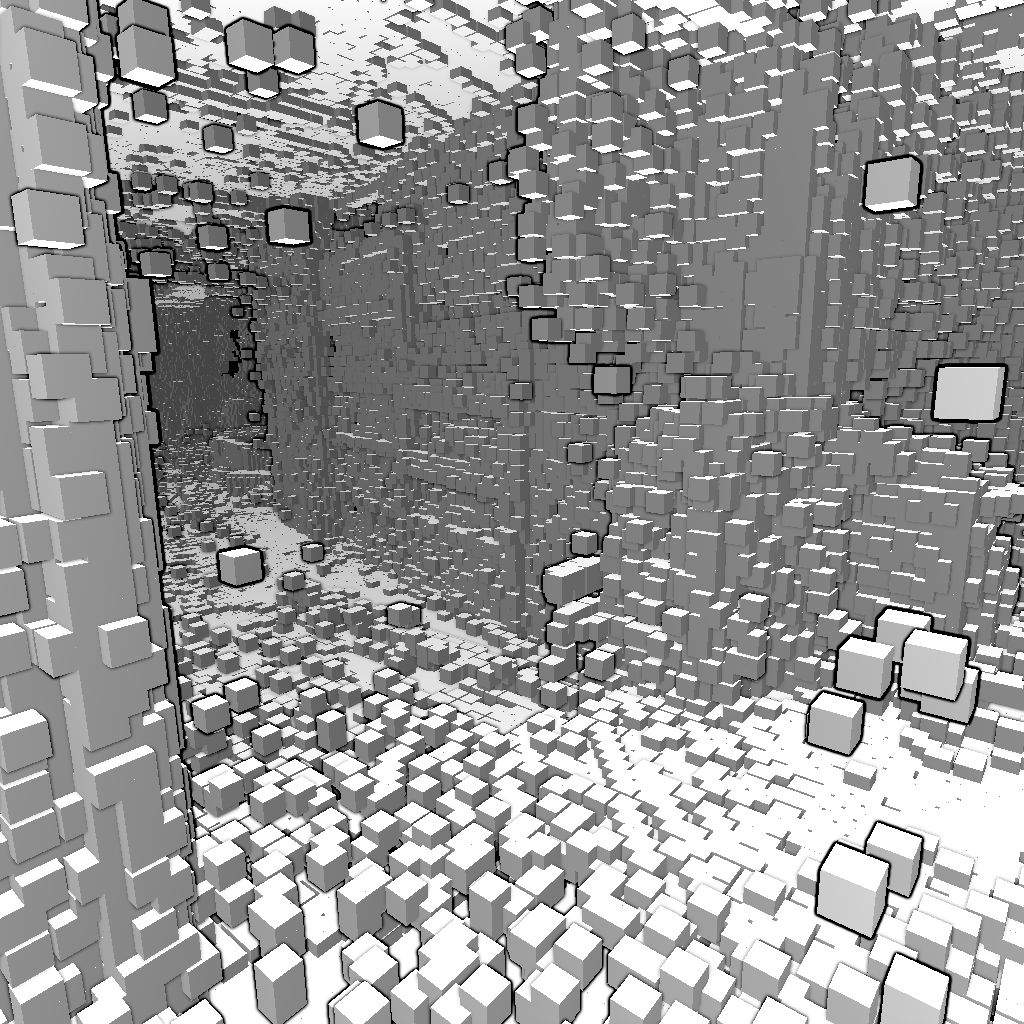
\includegraphics[width=0.99\textwidth]{figures/contributions/usar/rendering_voxel.png}}
    \caption{Full voxelized rendering with contours and depth enhancements.}
    \label{contributions:usar:rendering:voxel}
\end{subfigure}
\hspace*{2.5mm}
\begin{subfigure}[b]{0.21\textwidth}
    \fbox{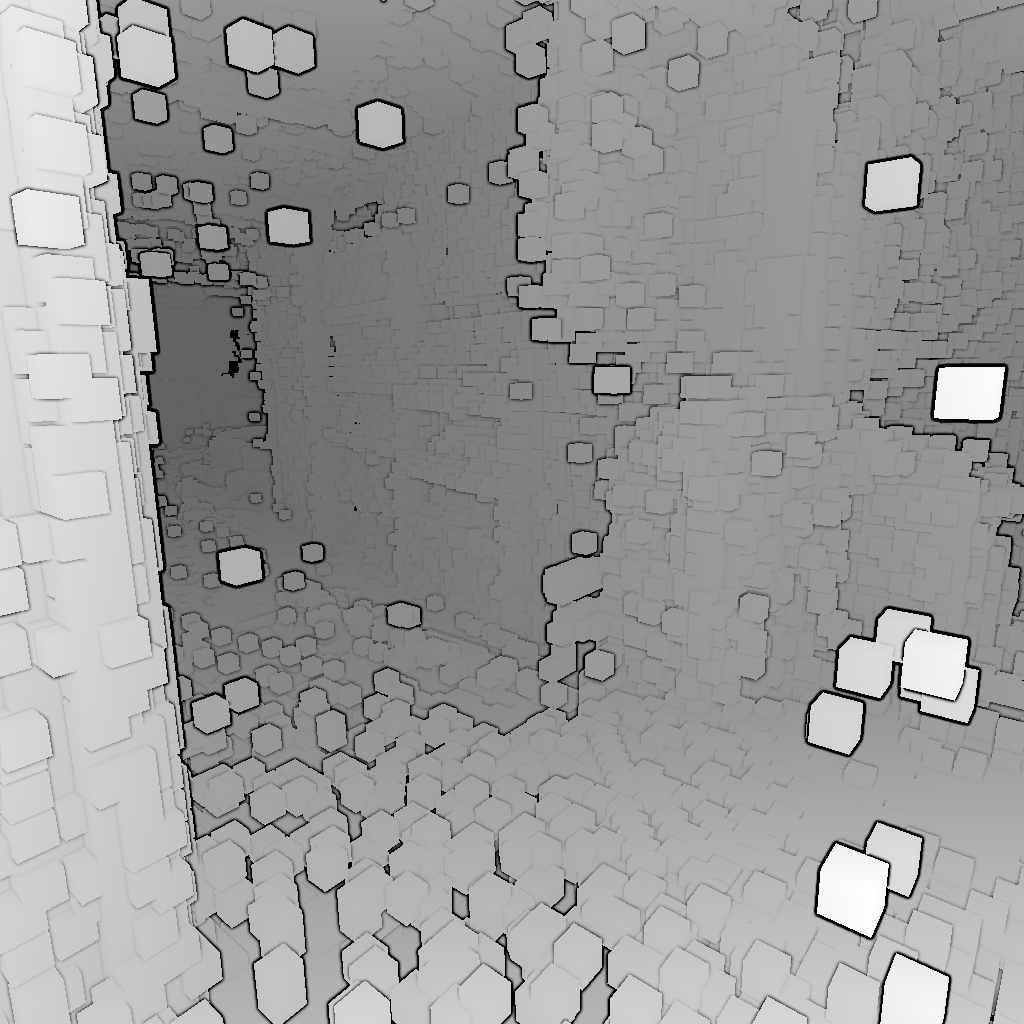
\includegraphics[width=0.99\textwidth]{figures/contributions/usar/rendering_depth.png}}
    \caption{Depth-image rendering that emphasizes the structure of the corridor.}
    \label{contributions:usar:rendering:depth}
\end{subfigure}
\caption{Comparisons of the different rendering methods.  A brute-force rendering of the original point cloud (a) is memory intensive and does not provide sufficient depth cues.  Using the binned point cloud and only applying Phong shading (b) is insufficient to detect corners and judge distance.  Using a contour rendering and depth darkening (c) it is possible to detect the structure of the corridor.  Using a different color mapping that emphasizes the depth information (d) provides additional information to the user.}
\label{contributions:usar:rendering}
\end{figure}

There are a number of technical challenges that are involved in providing an interactive rendering of the resampled point cloud together with a representation of the path classes and their analysis tools in the same view.  The following paragraphs cover the majority of challenges that had to be overcome.

\textbf{Point cloud visualization. }  The results of the original point cloud binning is a new, regularly spaced point cloud where the center of each voxel is represented by a single \nD{3} position and one global value for the voxel size.  This new point cloud is rendered by the GPU through the use of a geometry shader that creates an axis-aligned box for each of the incoming points.  In order to deal with occluding structures, for example roofs, the IC can interactively modify clipping planes that remove parts of the point cloud before rendering.  \fref{contributions:usar:rendering} shows different rendering stages and options that are applied to the visualization; to increase the spatial awareness, we apply a Phong shading based on the face of the cube using a camera-fixed setup of multiple light sources~\ref{phong1975illumination} and decided to employ two image-space enhancement methods.  The first method is a contour-enhancement that increases local contrast in areas of high depth changes~\etal \cite{luft2006image}.  It is a post-processing step that uses the depth buffer of the rendering, applies an unsharp masking on the value and then uses the result to visually enhance areas of the image with a high depth value gradient.  This allows the IC to intuitively gain a better understanding of the scene by emphasizing boundaries.  The second method that is also a image-based post-processing is a depth-based attenuation.  The farther a voxel is from the camera the darker it will be rendered, thus providing an intuitive distance cue for the IC.  As an optional method, we provide a simulated depth image resembling the output of range imaging cameras with which the IC is already familiar.

\textbf{Projective Texturing. }  An additional method to increase immersion the system uses a projective texturing to provide access to images from robots and provide more detailed information about the building~\cite{everitt2001projective}.  Provided the robot's orientation and location, information that is readily available, the images or videos are projected onto the voxels~\cite{zhao2005alignment}.  This method enables the optional inclusion of details where the IC requires them, without overloading the user with information.

\textbf{Bump Mapping. }  Even though it is possible to represent the occupancy values, which provide feedback about the data reliability, using color information, we found that in most situations the color information is used to display the location of hazardous environments instead.  Therefore, we use bump mapping that modifies the the face normals based on a structured noise pattern with periodic boundary conditions.  The displacement depends directly on the occupancy values.  Due to the oepration of the drones, the occupancy values consist mostly of radial patterns with decreasing occupancy towards the outside, thus leading to an automatic visual fading.

\textbf{Access path visualization. }  Each class of paths is represented in the \nD{3} rendering with a fixed color and posesses a vertical offset such that is it rendered on top of the voxel grid, rather passing through the center points.  The paths are rendered using Catmull-Rom spline interpolation in order provide a smooth path visualization and not capture the user's attention with jagged edges~\cite{catmull1974class}.  Furthermore, if multiple paths are passing though the same set of voxels in a row, they are offset horizontally to avoid cluttering and occlusion.  In addition to fixed colors for each path, the IC can select different coloring schemes to inspect attributes of the path that change along its length.  The color values mapped to the path can be any of the derived attribute and thus, for example, show the distance to the nearest hazardous environment for each point along the path or show how much space is available for a responder.  The IC can use selected paths for a virtual walk-through to inspect whether a path is feasible based on their own experience.  For these walk-throughs, the camera can be steered by the IC directly or it can follows a selected path automatically.

\textbf{Immersive Environments. }  The system also provides the IC with the option of rendering in an immersive environment, such as multi-pipeline display systems like planetariums or powerwalls, head-mounted displays, or fisheye projections.  This technique allows the IC to inspect the rendering using a head-mounted display on-sight, which increases the users performance in search tasks~\cite{pausch1997quantifying}.  We utilized this method to show a stereoscopic movie of two rescue scenarios to approximately 100 researchers at an international conference on rescue robotics.  

\begin{figure}
\centering
\fbox{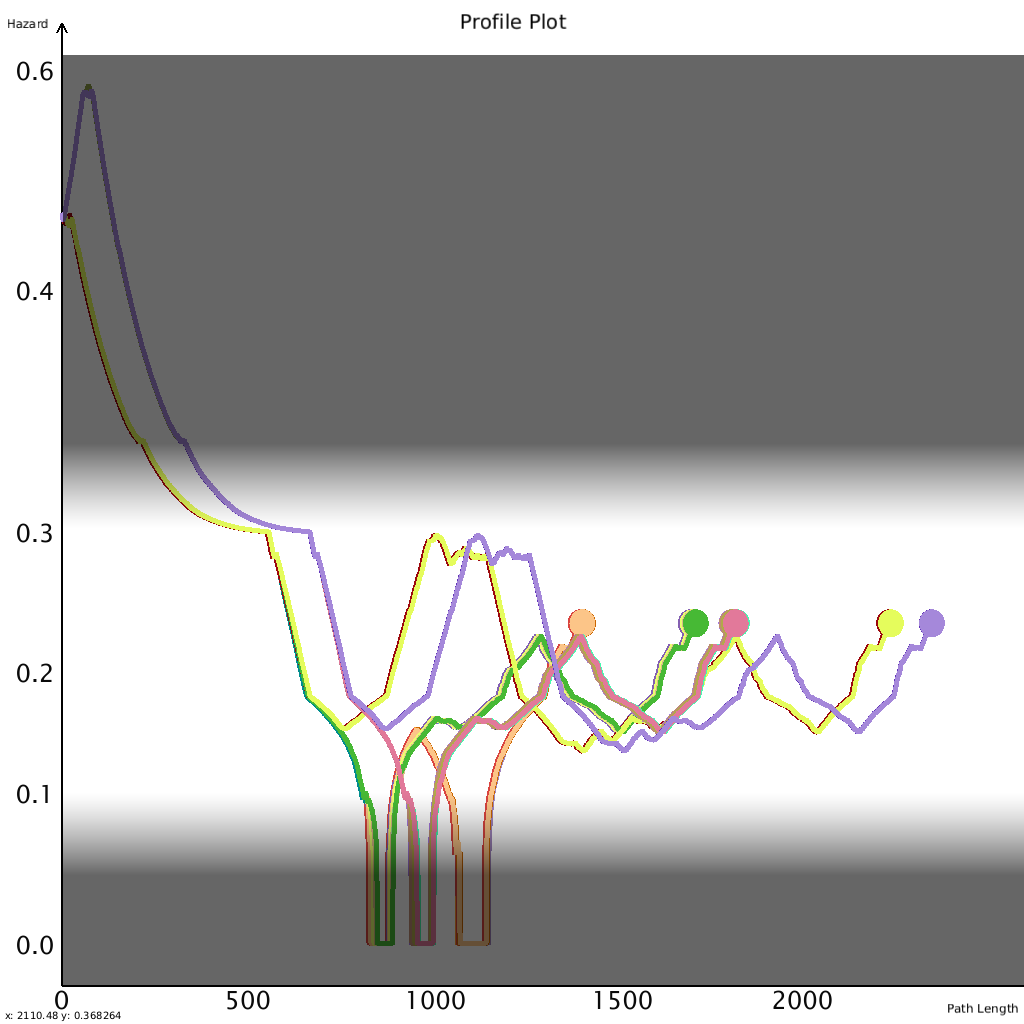
\includegraphics[width=0.75\textwidth]{figures/contributions/usar/profile_plot.png}}
\caption{The \emph{Profile Plot} component in the system shows the evolution of a user-selectable parameter over the length of all path classes.}
\label{contributions:usar:rendering:profile}
\end{figure}

\textbf{Profile Plot Remapping.}  One of the analysis views that is employed in a system is a modified line plot that enables the user to inspect a single value along the length of all path classes.  In order to make it easier for the user to compare paths, the ordinate axis value range has been modified to include a sub-linear, a linear, and a super-linear part.  The cut-off values can be chosen by the user to highlight different value ranges.  \fref{contributions:usar:rendering:profile} shows the \emph{Hazard Distance} mapped to the ordinate axis.  The transparency of the semi-transparent overlay shows the amount of performed remapping.

\subsection{System} \label{contributions:usar:system}
\begin{figure}
\centering
\fbox{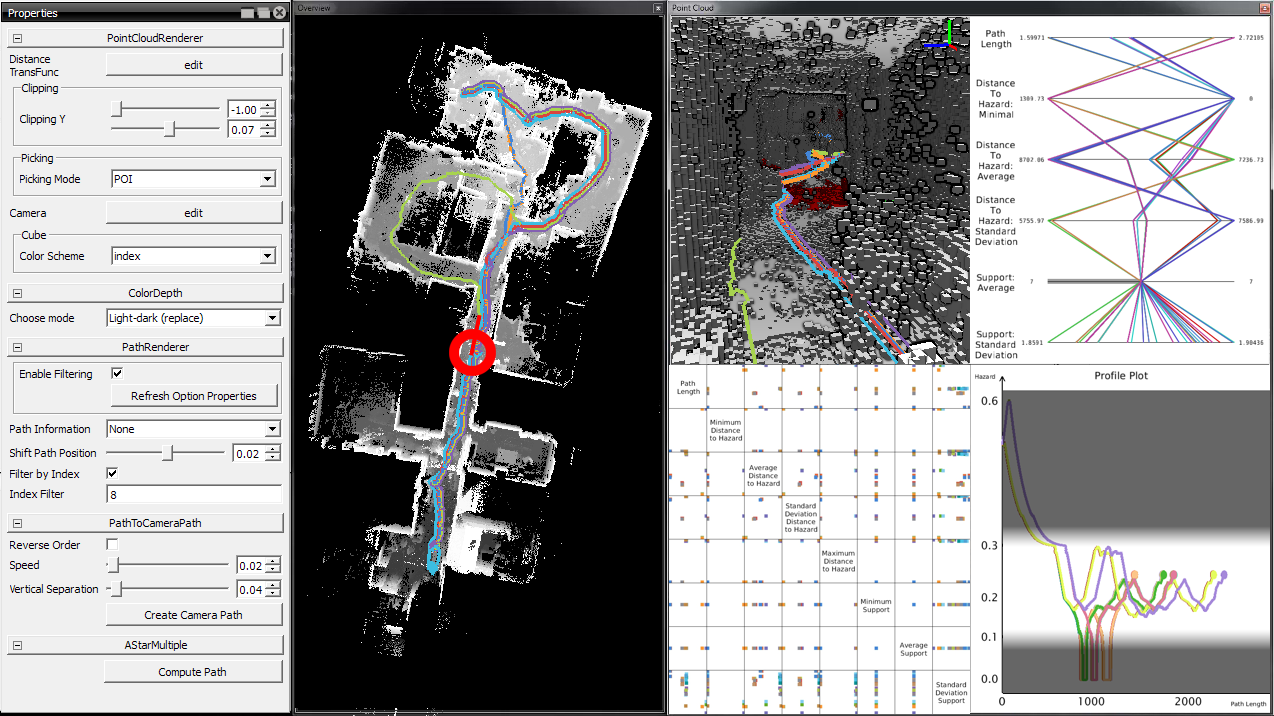
\includegraphics[width=0.99\textwidth]{figures/contributions/usar/system.png}}
\caption{The overview of the system that consists of four views, the rendering view (top left), the profile plot (bottom right), the parallel coordinates plot (top right), and the scatter plot matrix (bottom left).}
\label{contributions:usar:system:system}
\end{figure}

The entire system consists of four views, the \emph{Rendering View}, \emph{Profile Plot}, \emph{Parallel Coordinates Plot}, and the \emph{Scatterplot Matrix}, which are organized in a single application (see \fref{contributions:usar:system:system}).  The \emph{Rendering View} provides the user with an interactive view of the point cloud data in which they can select paths, annotate voxels, and inspect the building in the \nD{3} environment.  The other three views are dedicated to support the IC with the analysis of the available path classes.  The rendering view (top left) provides the user with a global overview of the structure and the path classes that traverse it.  The user can select paths in this view to highlight them in all views.  The profile plot (bottom right) shows how a parameter selected by the user changes over the entire length of all path classes.  This view can be easily used by the IC to filter paths by their maximum or minimum values and also see general trends.  The parallel coordinates plot (top right) shows all derive attributes for all path classes at the same time in order to provide the user with an overview of potential correlation between parameters.  Finally, the scatter plot matrix (bottom left) shows the combination of all derived parameters in case it is needed for the IC.


\subsection{Evaluation} \label{contributions:usar:evaluation}
\begin{figure}
\fbox{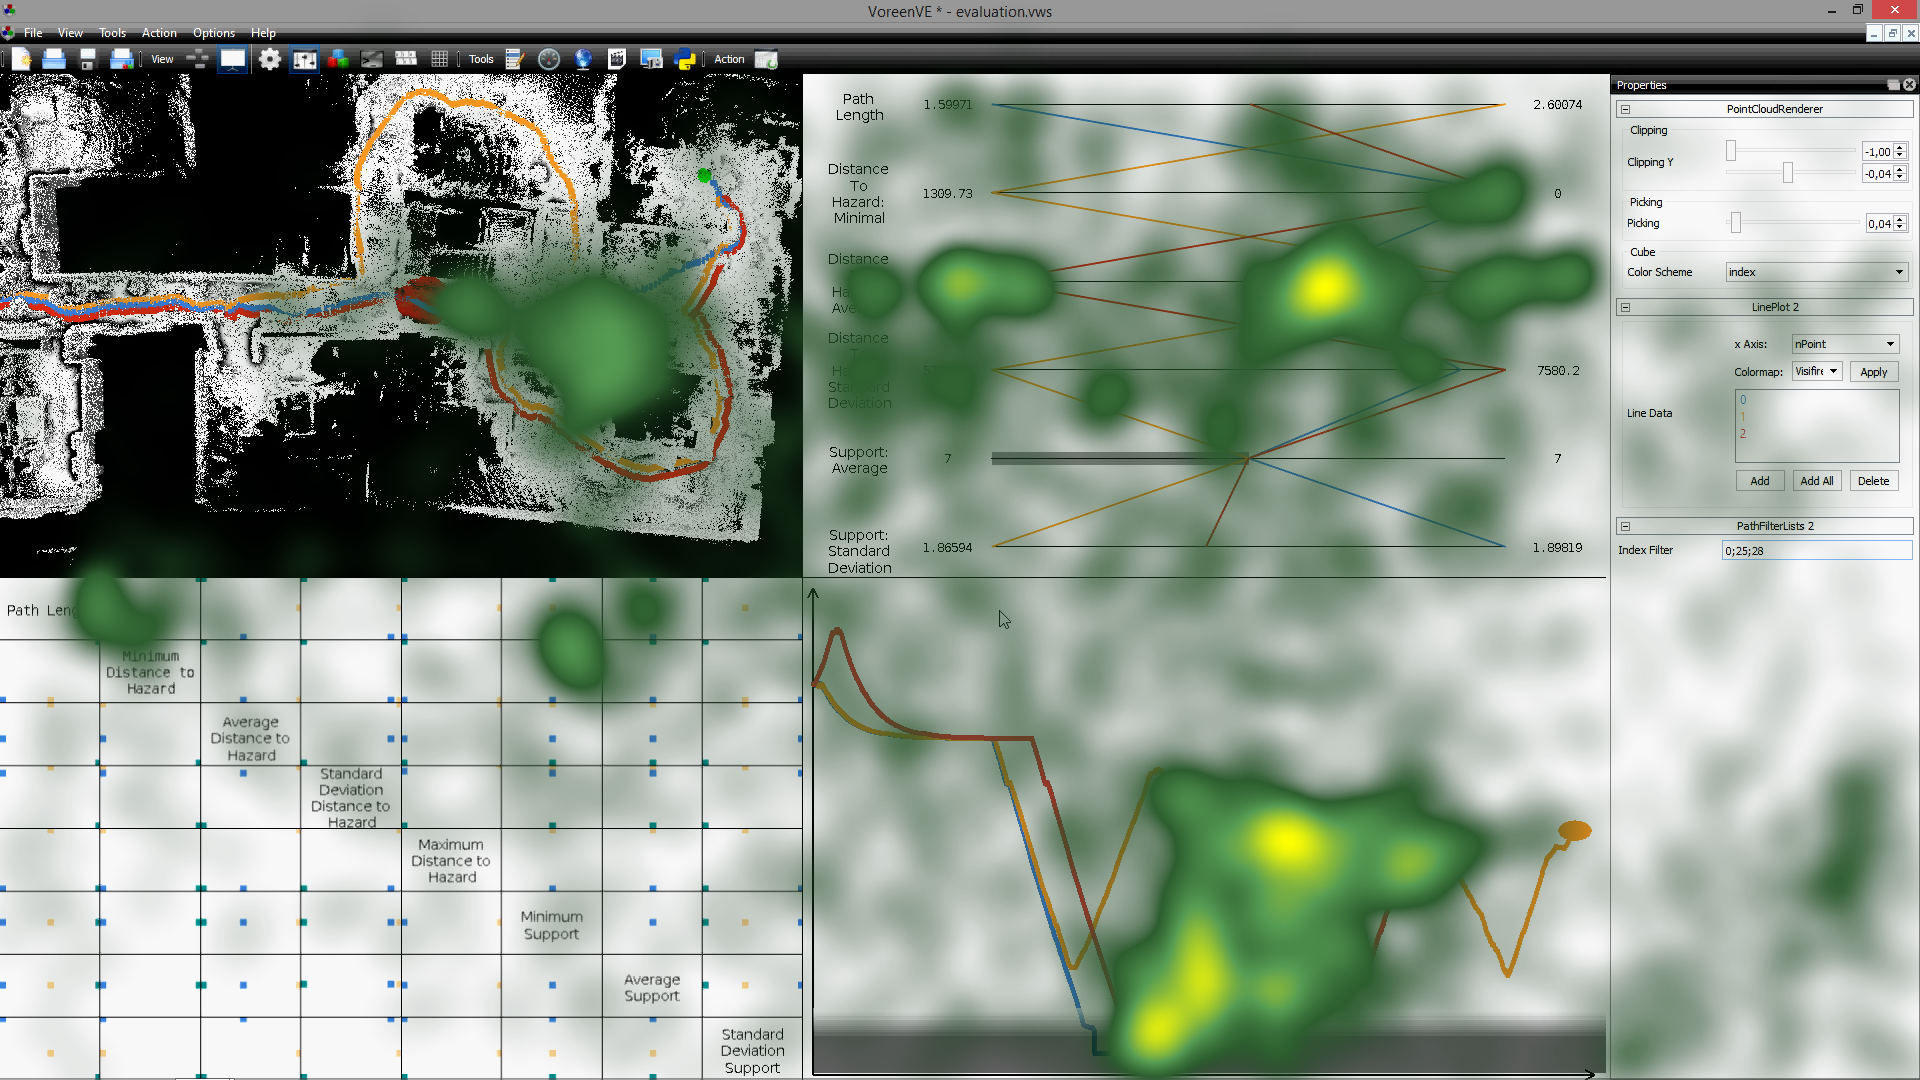
\includegraphics[width=0.99\textwidth]{figures/contributions/usar/heatmap.png}}
\caption{A heatmap showing the amount of gaze points of one expert while analying a use case over the course of about 15 minutes.}
\label{contributions:usar:system:heatmap}
\end{figure}

The usability and usefulness of the system was tested using two evaluations.  The first evaluation was performed early in the development of the system and consisted of an online questionnaire that was completed by nine international urban search \& rescue experts, composing a mix of emergency responders, researchers, and a consultant for technical relief agency.  During this evaluation, the experts inspected images and videos of the system being used before answering questions and providing feedback.  The results of the seven experts that completed the evaluation are reported in detail in \paperef{paperD}.  The second evaluation was performed with four experts from the Swedish Civil Contingencies Agency~(MSB)~and involved an interactive session with the system which included a think-aloud usage supplemented by an eye-tracking study~(see \fref{contributions:usar:system:heatmap}).  During the 45 minute usage of the system, the experts were asked to familiarize themselves with the application and inspect one of the prepared use cases and make decisions about potential paths for responders.  The results of these evaluations are reported in \paperef{bock16visualization}.





\section{Astronomical Visualization} \label{contributions:astro}
\begin{wrapfigure}{o}{0.4\textwidth}
\centering
\fbox{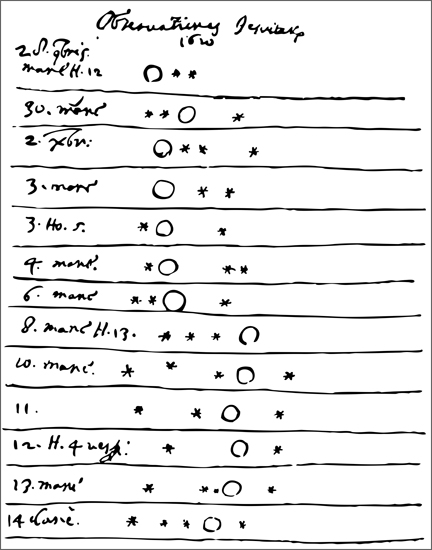
\includegraphics[width=0.38\textwidth]{figures/contributions/astro/galileo.jpg}}
\caption{The original drawings by Galileo Galilei of the movements of Jupiter's main moons enabled the later realization that these are not stars but objects orbiting Jupiter and thus informed the discovery that the Earth orbits the Sun, not vice versa.}
\label{contributions:astro:galileo}
\end{wrapfigure}

Visualization has been employed in the field of astronomy and astrophysics almost since its appearance.  An early example are the drawings by Galileo Galilei that, for the first time, systematically document the movements of Jupiter's moons around Jupiter.  Analyzing these movements enabled him to discover the true helioscentric structure of the solar system (see \fref{contributions:astro:galileo})~\cite{galilei1610sidereus}.  Especially since the introduction of computers into the visualization work, these two fields have expanded rapidly in concert, and these days visualization systems are used in a large number of applications that span the entire spectrum from intial knowledge discovery, such as a scientist analyzing simulation results, all the way to public dissemination, such as Jim Blinn's 1978 animations of the Voyager spacecraft.

The contributions presented in this thesis follow along the same two directions as these historical examples, the use of visualization as a support for hypothesis generation, in this case in the context of time-varying ensemble simulations of the solar system (\SC{contributions:astro:spaceweather}), and its use to communicate engineering or scientific endeavors to the general public, through the development of a freely available software tool called \emph{OpenSpace}~(\SC{contributions:astro:openspace}).


\subsection{Space Weather Visualization} \label{contributions:astro:spaceweather}
The work leading to \paperef{paperF} was performed in close collaboration with the scientists at the Community Coordinated Modeling Center~(CCMC) at NASA Goddard Space Flight Center that started two years prior~\cite{tornros2013interactive, bock14vcmass} and is concerned with the verification of space weather simulations.


\subsubsection{Domain and Scientific Problems} \label{contributions:astro:spaceweather:background}
The CCMC generates time-varying ensemble simulations of the plasma conditions in the solarsystem in order to further the study of \emph{space weather}, which descibes its effects on spacecraft, planetary bodies, and human society at large.  The Sun is constantly ejecting charged particles into the solar system and parameters of this plasma, such as density, velocity, distribution, and its interaction with magnetic fields and planetary bodies, have a large effect humans and our technological devices.  One type of increased activity, called coronal mass ejections (CMEs), can have devastating effects on human technology as 1. electronics can be destroyed by fast-moving charged particles, which also pose danger to astronauts travelling outside Earth's protective magnetic field, and high currents can be induced by Earth's rapidly changing magnetic fields as it reacts to these particles.  Other effects are the thermal expansion of Earth's atmosphere and thus increased drag, which can drastically reduce the lifetime of operational satellites~\cite{knowles2001effect}.  An example of the former is Telstar 401, a satellite that was rendered inoperable in 1997 due to a geomagnetic storm~\cite{sabol1998analysis}.  An example of the latter is the induction of currents in long metal structures on the surface of Earth that can deteriorate, for example, railroads or pipelines~\cite{pirjola1999power}.  The most destructive, however, is the presence of induced current in high-voltage power lines that are directly connected to sensitive transformers which can be overloaded and destroyed by the excess energy.  In 2003, Llyod's prediced that if the strongest CME ever recorded, the Carrington Event from 1859, were to occur, the damages to the global economy would be around \$2 trillion and could lead to power outages of up to 2 years until destroyed transformers are replaced~\cite{maynard2013solar}.  The strength of a CME's interaction with Earth's magnetic field is measured by its geoeffectivity and depends, among others, on its speed and the angle between the CME's and Earth's magnetic fields, which is a separate simulation parameter.  In the simulations performed at the CCMC, three angles are simulated, 90\textdegree , 135\textdegree , and 180\textdegree .

\begin{figure}
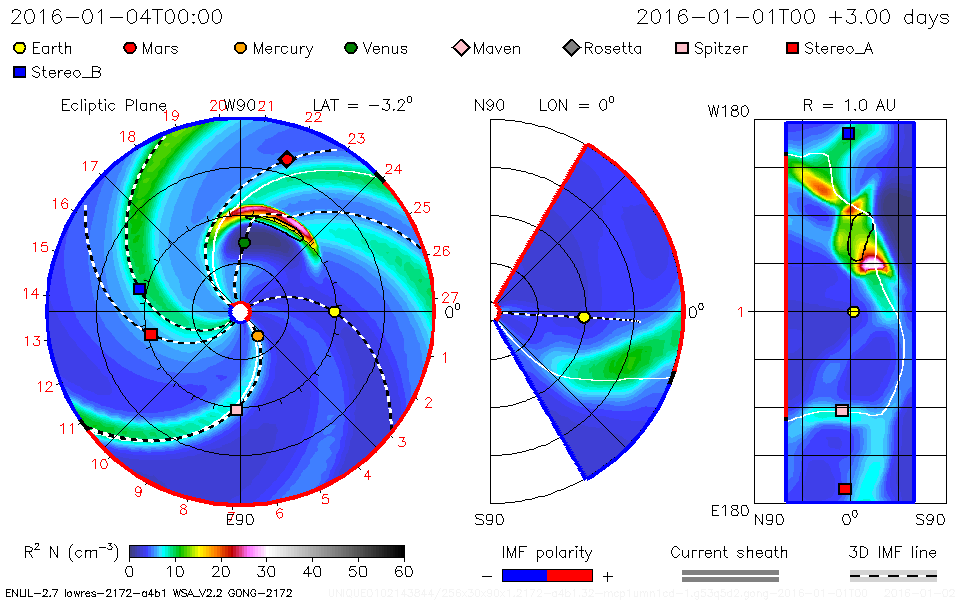
\includegraphics[width=\textwidth]{figures/contributions/spaceweather/enlil.png}
\caption{A single ENLIL simulation timestep with a coronal mass ejection in flight.  In previous work, the volumetric data was sliced along the ecliptic plane (left), the north-sound plane passing through Earth (middle), and a plane of constant radius (right).  These slices make it difficult to analyze the three dimensional structure of the CME.}
\label{contributions:astro:spaceweather:enlil}
\end{figure}

These scenarios can be mostly mitigated if operators are informed of incoming CMEs as electrical hardware can be temporarily disabled and astronauts can seek shelter in protected areas.  Therefore, it is of paramount importance to provide reliable prediction of these types of solar events.  Currently, most CME predictions are created using a time-varying magnetohydrodynamic (MHD) volumetric simulation called ENLIL in which the input parameters are derived from real-time sun-observing satellite imagery~\cite{mays2015ensemble}.  These simulations create an ambient background flow of charged particles from the Sun and inject a CME event~(a symmetric cone is assumed in the model)~that is constained by the available satellite imagery.  The free parameters determined by the human operators are the direction (\emph{logitude} and \emph{latitude}), the \emph{speed}, and the \emph{opening angle}.  Naturally, manual segmentations are not necessarily accurate and can lead to prediction errors that are independent from the accuracy of the simulation model itself.  This variation is offset by using ensemble simulations to vary the free parameters and perform a simulation for each parameter combination.  It then becomes possible to analyze the predictions of the simulations and compare these to real-world measurements and, thus, enables the scientists to gain more insight into potential errors in the simulation models that are independent from the human inputs that were used to create the ensemble simulations.

\begin{figure}
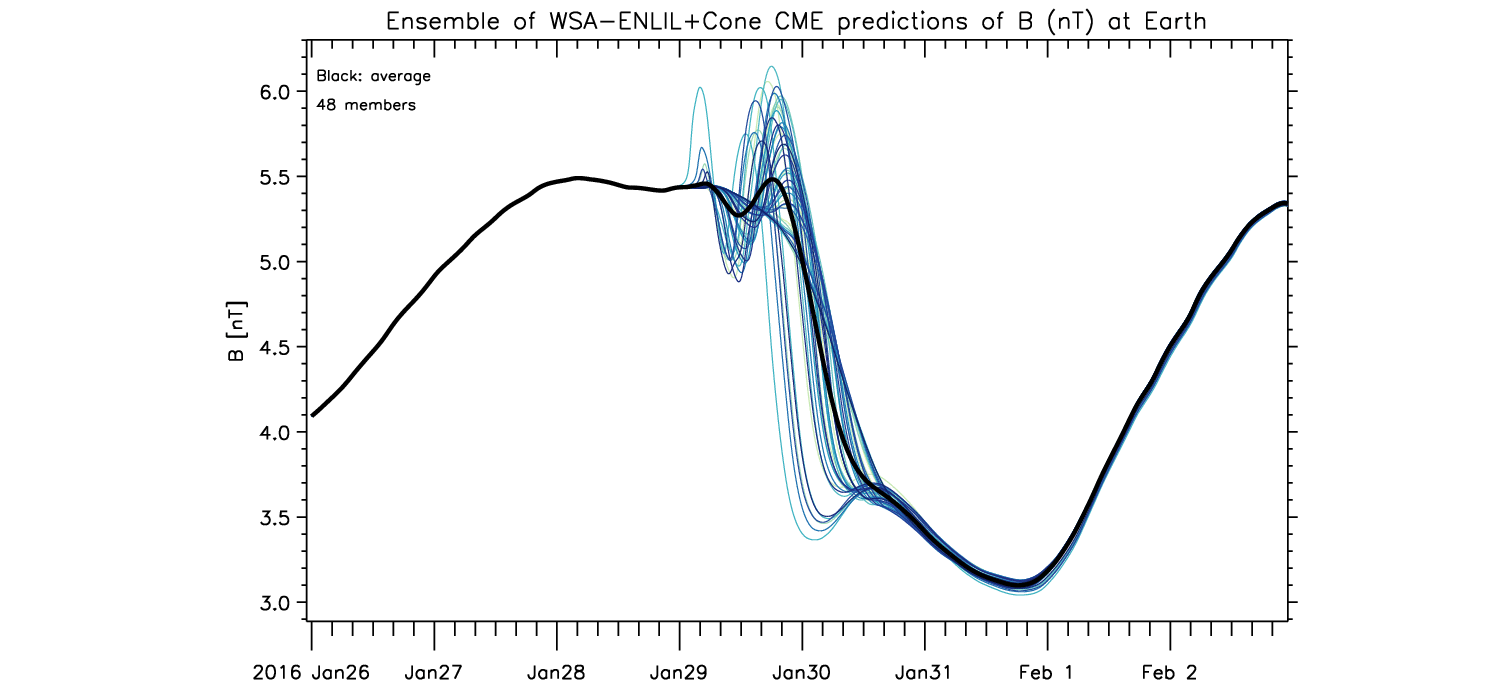
\includegraphics[width=\textwidth]{figures/contributions/spaceweather/ensemble.png}
\caption{The method of presenting the time-varying ensemble results makes comparative analysis difficult as the scientists have to manually compare a set of line plots in order to reach a conclusion.}
\label{contributions:astro:spaceweather:ensemble}
\end{figure}


\subsubsection{Application Requirements} \label{contributions:astro:spaceweather:requirements}
The work in \paperef{paperF} was performed in order to provide the scientists with better tools to analyze these ensemble simulations of past CME events in detail in order to inform the development of the simulation models and increase the accuracy of their predictive use.  Previously, this analysis was done using seperate tools~(see Figures~\ref{contributions:astro:spaceweather:enlil} and~\ref{contributions:astro:spaceweather:ensemble})~that prevent the scientists from easily determining the root causes of simulation errors as multiple, unconnected views had to be employed.  The goal for this application is to create a single system that combines all information about the ensemble simulations and provides the domain experts with the tools to easily determine the quality of the ensemble simulations and inspect their volumetric simulations in order to view the \nD{3} structure of the CME.

This approach is based on having access to ground-truth measurements of the arrival time, speed, and geoeffectivity recorded on or close to Earth as well as being able to derive values from the simulations and compare these on different granularities.  The predictive strength of the simulation depends on the difference between the simulated quantity and the ground truth.  The arrival time and geoeffectivity are only known for a single measurements, but the CME is visible in the optical telescopes on-board the observing space craft, making it feasible to compare the velocity of the CME at multiple points during transit.

This leads to a series of challenges that the system presented in \paperef{paperF} addresses.  The system must present the user with the ability to quickly inspect the relationship between simulation input parameters and the prediction accuracy of each ensemble member.  This requires an intuitive visual representation of the \nD{4} input parameter space (\textbf{C1}).  The user must be capable to inspect the evolution of individual ensemble members over time.  This particularly requires the comparison of reconstructed velocity information with the simulated velocity over a large number of timesteps and taking into account the different time resolutions of available data.  This requires the extraction of comparable velocities from available satellite images as well as the ensemble simulations (\textbf{C2}).  For single timesteps of individual ensemble members, it must be possible for the user to view a representation of the volumetric data in its correct relation to the satellites, the Sun, and Earth, making it necessary to accurately position astronomical positions with respect to the simulation data and be able to render transparent geometries combines with multi-volume rendering (\textbf{C3}).


\subsubsection{Ensemble Glyph Mapping} \label{contributions:astro:spaceweather:glyphs}
\begin{figure}
\centering
\begin{subfigure}[b]{0.32\textwidth}
    \fbox{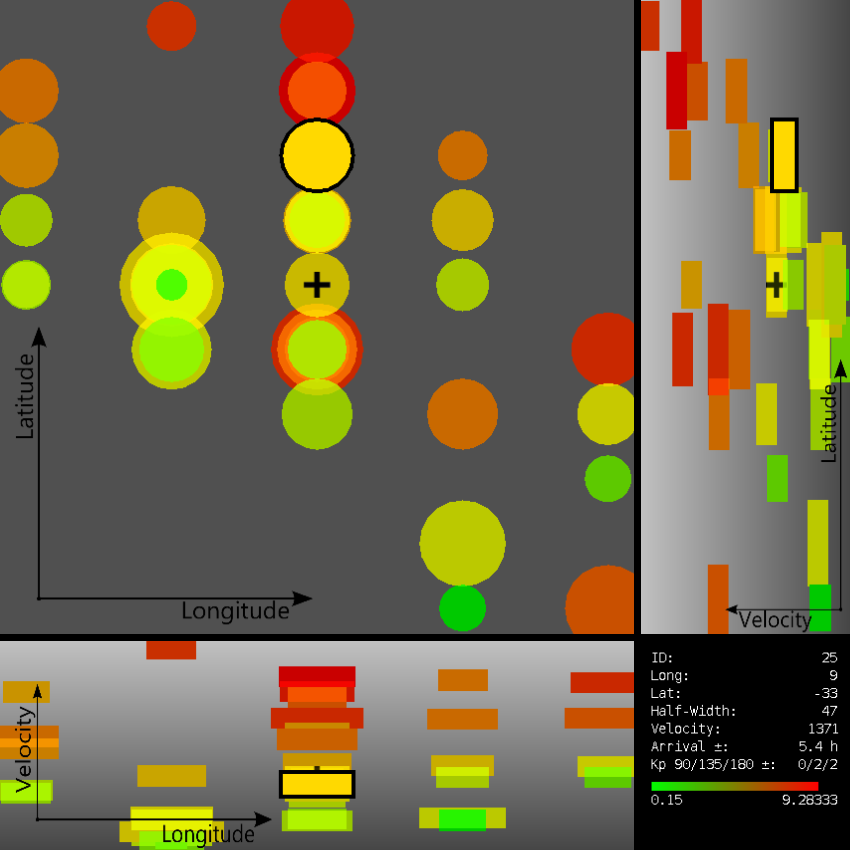
\includegraphics[width=0.99\textwidth]{figures/contributions/spaceweather/ensemble_arrival.png}}
    \caption{Arrival time prediction}
    \label{contributions:astro:spaceweather:ensemble:arrival}
\end{subfigure}
\hspace*{1cm}
\begin{subfigure}[b]{0.32\textwidth}
    \fbox{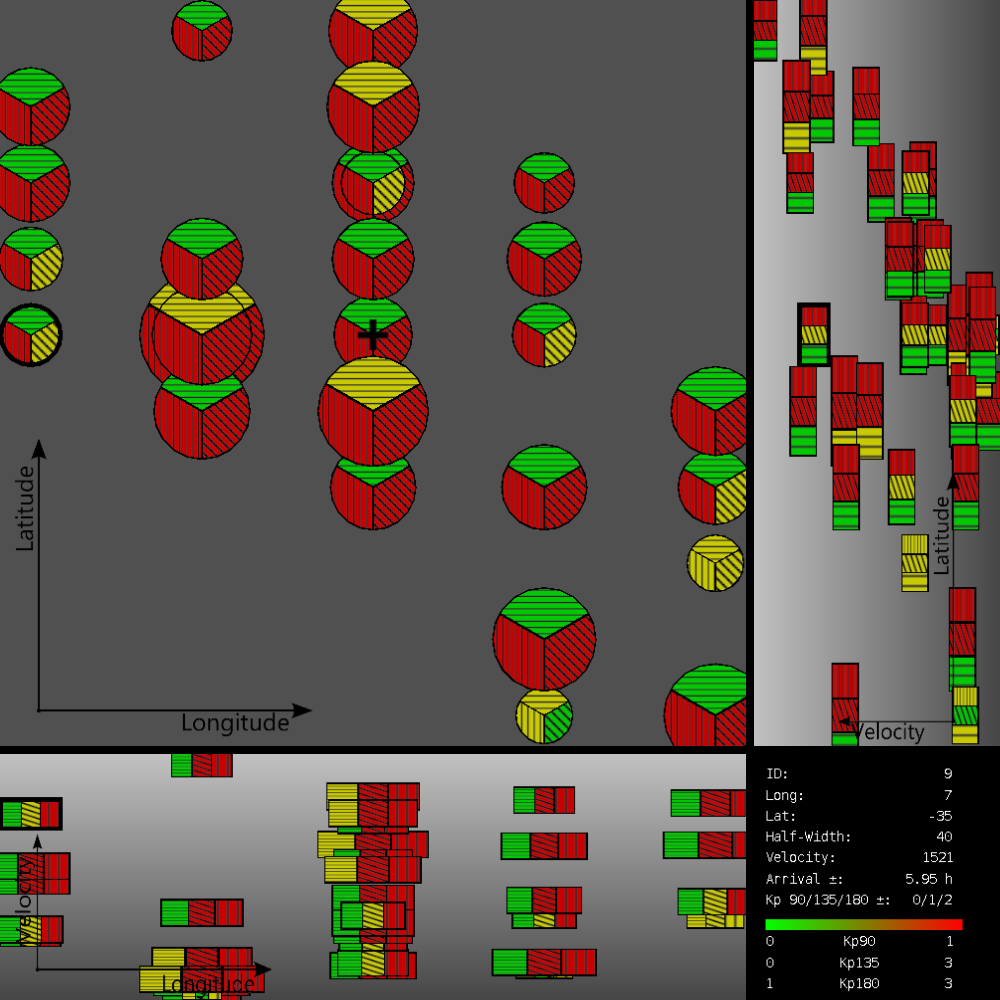
\includegraphics[width=0.99\textwidth]{figures/contributions/spaceweather/ensemble_kp.png}}
    \caption{Geoeffectivity prediction}
    \label{contributions:astro:spaceweather:ensemble:kp}
\end{subfigure}
\caption{These views show the two modes of the glpyh-based ensemble member representation.  The free parameters \emph{longitude}, \emph{latitude}, \emph{velocity} (location), and \emph{opening angle} (size) are mapped in three views and the accuracy of arrival time (a) and three geoeffectivities (b) are shown color coded.}
\label{contributions:astro:spaceweather:ensemble}
\end{figure}

A design requirement for the system was the ability to easily inspect potential correlations between the input parameters and the quality of the simulation results, which previous systems did not support.  For each ensemble member, there are four input dimensions, the \emph{longitude}, \emph{latitude}, \emph{velocity}, and \emph{opening angle}, and four quality values, each differences between the predicted and measured values, \emph{arrival time}, and \emph{geoeffectivity} for three clock angles 90\textdegree , 135\textdegree , and 180\textdegree .  \fref{contributions:astro:spaceweather:ensemble} shows the \nD{2} glyph-based projections that were designed.  For all subviews, the size of the glyphs correlates with the opening angle of the ensemble member, a bigger opening angle resulting in a larger glyph.  Some ensembles also contain an additional, average ensemble run, which is denoted with a $+$ symbol.  If the user selects an ensemble member, it is highlighted in all three views.  The main view (top left) shows the ensemble members mapped into the longitude, latitude space.  The mapping is performed linearly using the minimum/maximum values of all ensemble members.  The glyphs of ensembles with larger opening angles are rendered first, such that smaller angles overpaint and are still visible if multiple simultions were performed at the same location.  The other two views provide replace one of the longtitude, latitude information with the velocity of the CME.  The views are arranged such that the remaining quantity acts as a projection of the main view with the velocity being the distinguishing factor.  Finally, an additional window provides information about the currently selected ensemble member in order to provide the actual numerical values.

The entire view can be switched to show either the accuracy in CME arrival time or its geoeffectivity.  In both cases, color represents how well the simulation agrees with the measured data.  This value is normalized to $0$ and the maximum error for the entire ensemble and shown using a green-red color scale.  For the arrival time, the entire glyph is colored uniformly (see \fref{contributions:astro:spaceweather:ensemble:arrival}).  For the geoeffectivity, there are three predictions for each ensemble members and the glyph is, thus, split into three segments.  The magnetic angle for each part is represented by the angle of the textured lines in that segment.

\subsubsection{Optical Flow Analysis} \label{contributions:astro:spaceweather:opticalflow}
\begin{figure}
\centering
\begin{subfigure}[b]{0.32\textwidth}
    \fbox{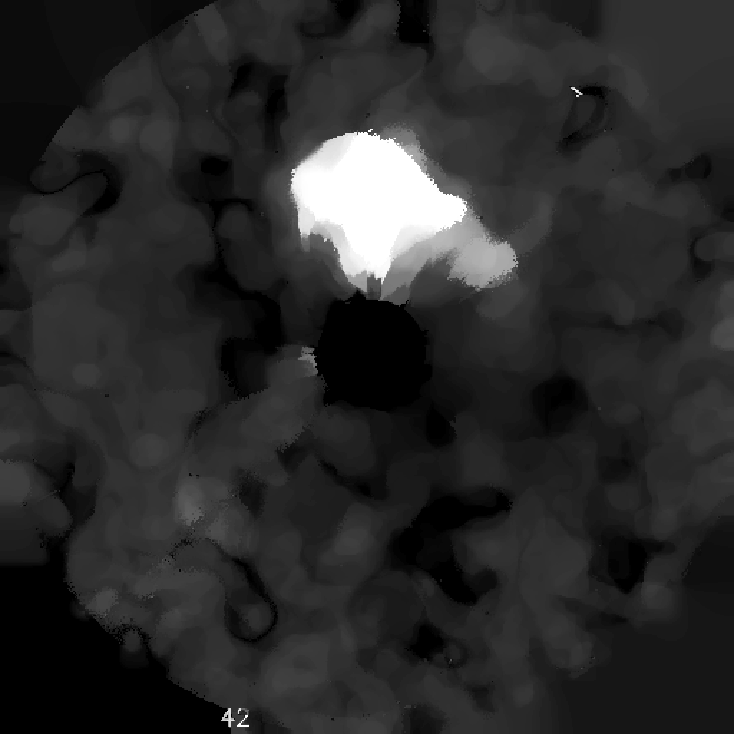
\includegraphics[width=0.99\textwidth]{figures/contributions/spaceweather/optical_flow.png}}
    \caption{Length of the optical flow derived velocity vector for each pixel in the Cor2 image.}
    \label{contributions:astro:spaceweather:velocity:opticalflow}
\end{subfigure}
\hspace*{1cm}
\begin{subfigure}[b]{0.32\textwidth}
    \fbox{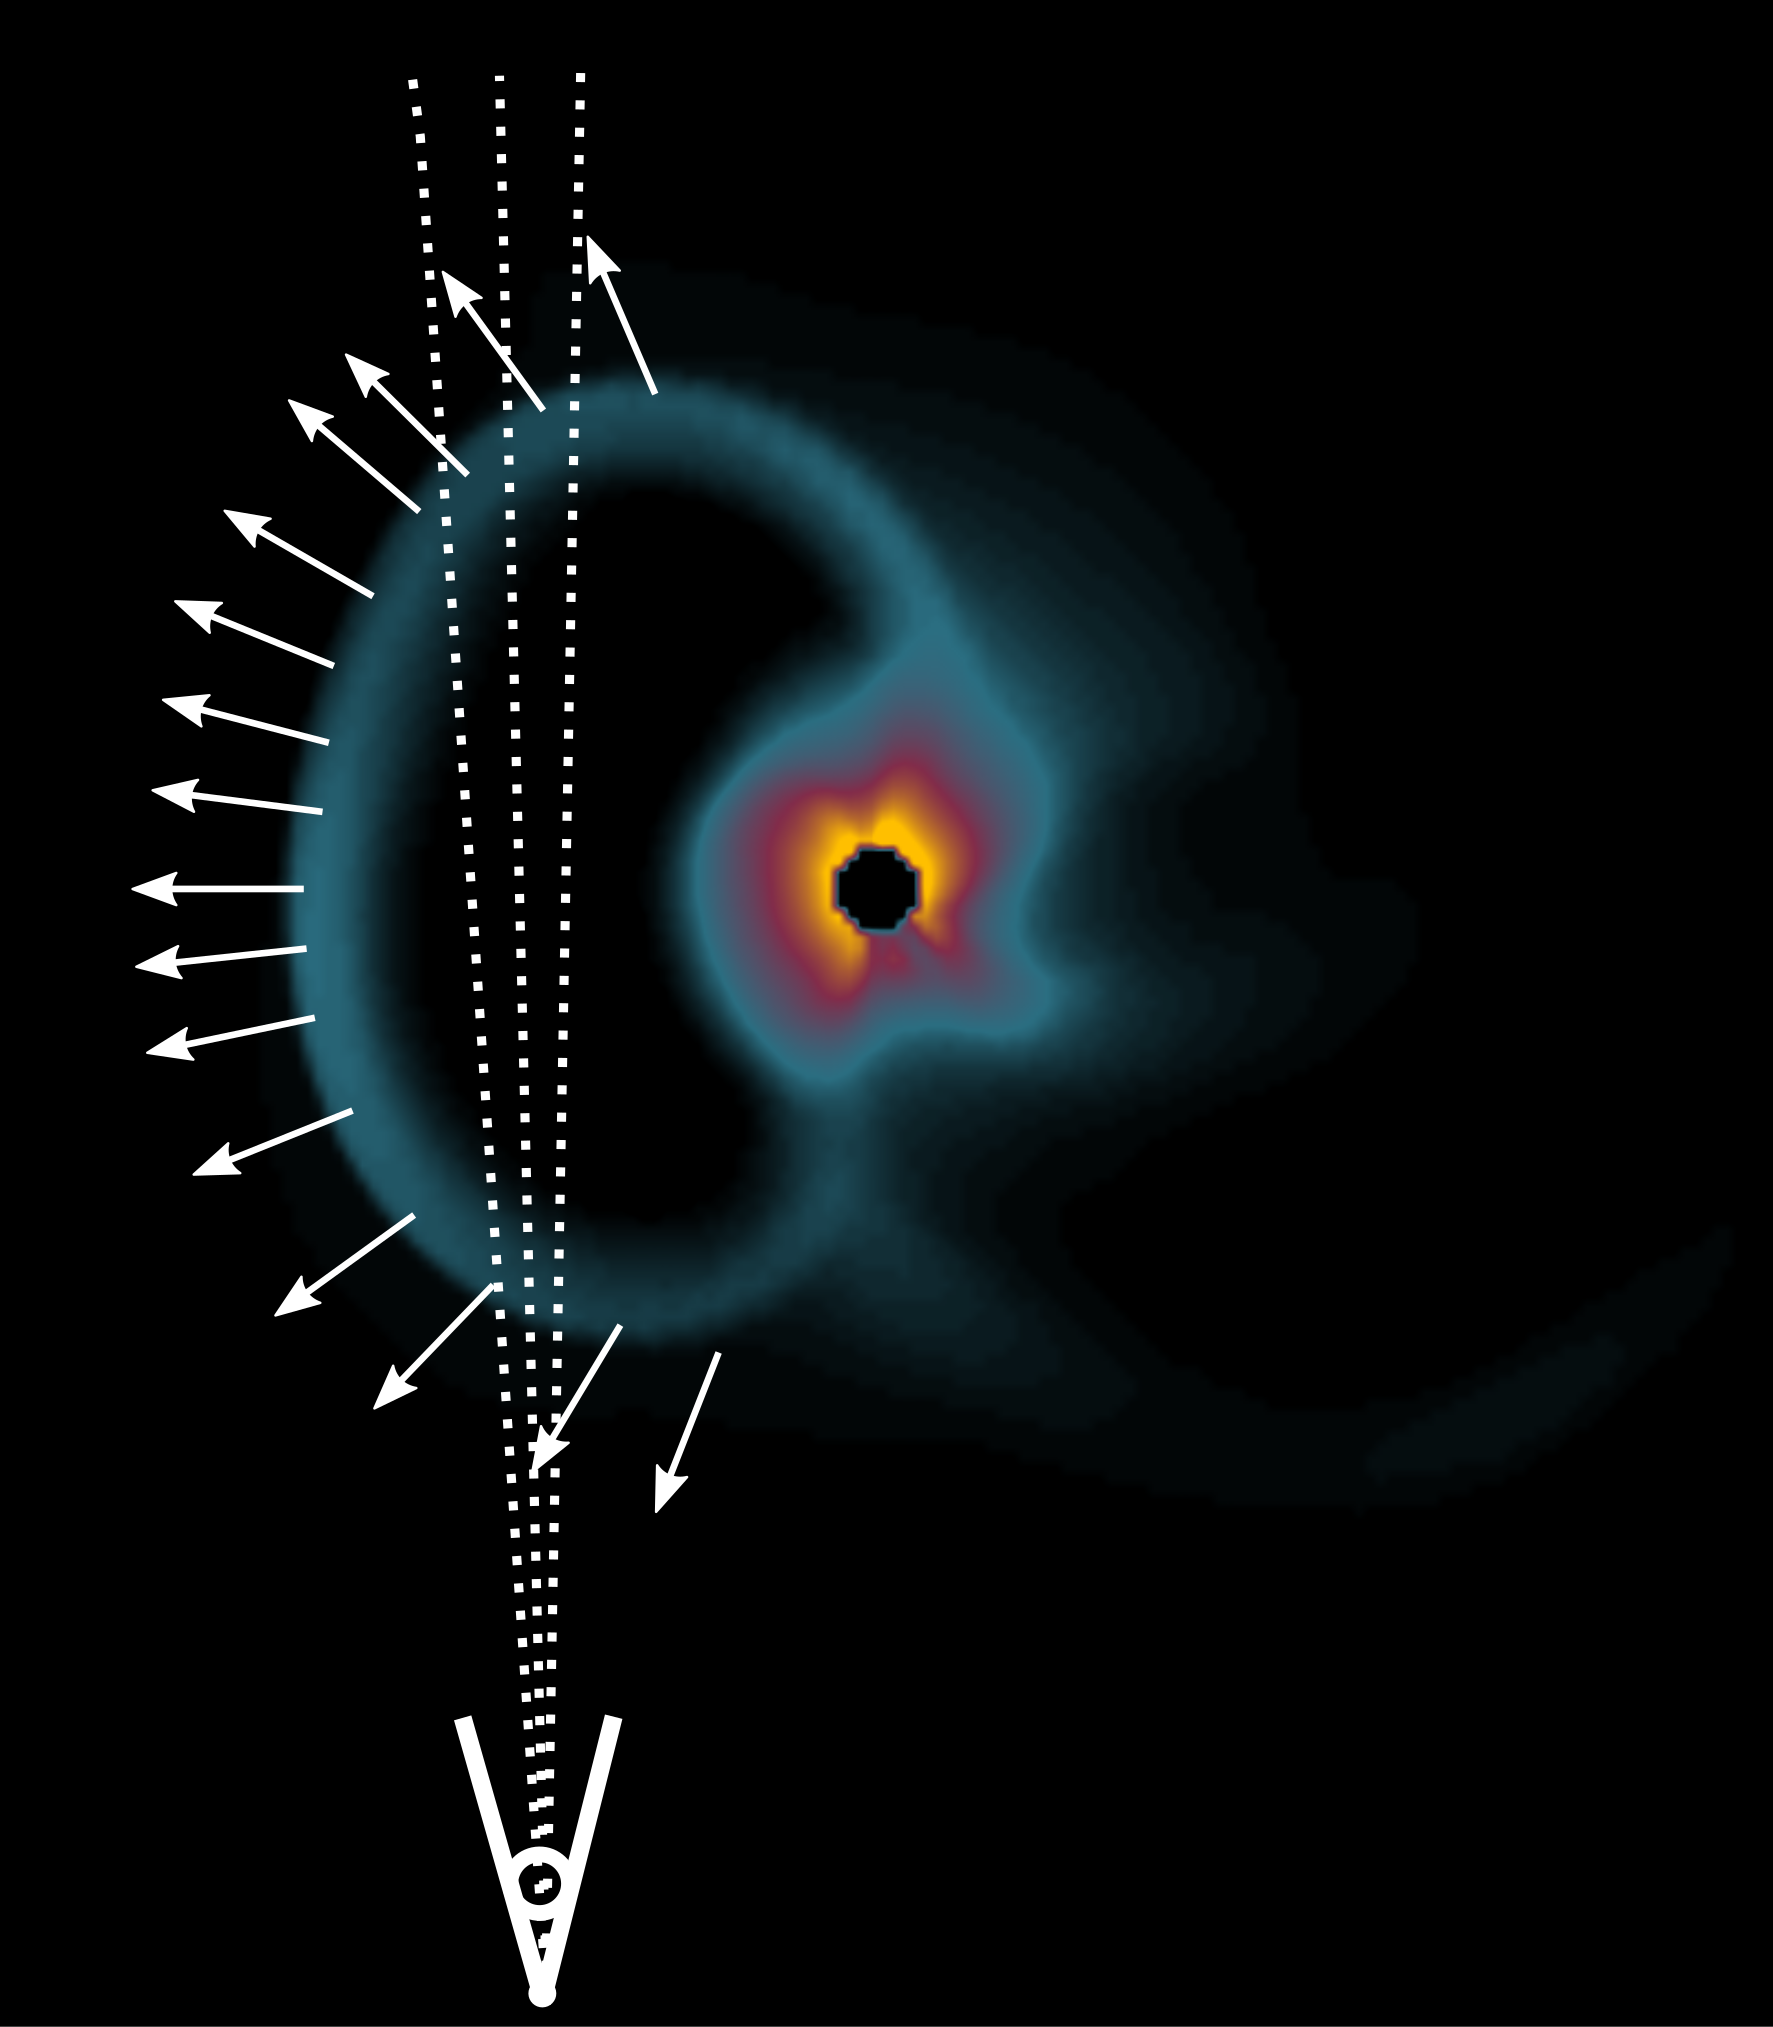
\includegraphics[width=0.99\textwidth]{figures/contributions/spaceweather/cme_velocity.png}}
    \caption{Illustration of the projection of the volumetric velocity field along a view ray.}
    \label{contributions:astro:spaceweather:velocity:simulation}
\end{subfigure}
\caption{The construction of a timeline of velocities for each ensemble member includes extracting the velocity from each subsequent pair of satellite images for each instrument~(a), as well as retrieving the simulated velocity for each position from the volume~(b).}
\label{contributions:astro:spaceweather:velocity}
\end{figure}

% In order to address the technical challenge \textbf{C2}, i
It was necessary to reconstruct the CME's velocity from the available satellite images.  An optical flow algorithm computes a vector field describing the movement of objects between two input images and thus describe how individual features move between subsequent frames.  While this has been shown to work with solid objects, Colaninno \etal also found that it was feasible to determine the tangengial velocity of CME shock fronts using optical flow analysis~\cite{colaninno2006analysis}.  In our case, we use subsequent images from the major sun-observing instruments (Cor2, HI 1, HI 2, and LASCO C3) and compute the optical flow for each pixel using the algorithm presented by Sun \etal ~\cite{sun2010secrets}~(see \fref{contributions:astro:spaceweather:velocity:opticalflow}).  In order to retrieve a single, representative velocity for the CME, the vector field is first replaced by a scalar field of their lengths.  Then, the bottom 75\% of data values are discarded in order to remove the slow-moving background data and, finally, a representative velocity value is computed by averaging the remaining 25\% of values.

In order to be able to retrieve a comparable velocity from the volumetric simulations, it is necessary to reproject the velocity values of the simulation for each instrument.  For this, the simulation was rendered using volumetric raycasting with the camera set to the satellite's location and its field-of-view.  For each pixel, the simulation's velocity is sampled and a running average of velocities is constructed~(see \fref{contributions:astro:spaceweather:velocity:simulation}).  As the optical flow algorithm can only detect tangential velocity, the simulated velocity first has to be projected into the tangential plane before adding.  Then, similar to the optical flow, the final velocity is the average of the top 25\% of the velocity vector's lengths.


\subsubsection{Rendering} \label{contributions:astro:spaceweather:rendering}
\begin{figure}
\centering
\fbox{\includegraphics[width=0.99\textwidth]{figures/contributions/spaceweather/rendering.png}}
\caption{The rendering of this scene requires the support of accurate locations as well as the ability to render transparent geometry together with the volume data.}
\label{contributions:astro:spaceweather:rendering:rendering}
\end{figure}

\begin{figure}
\centering
\begin{subfigure}[b]{0.32\textwidth}
    \fbox{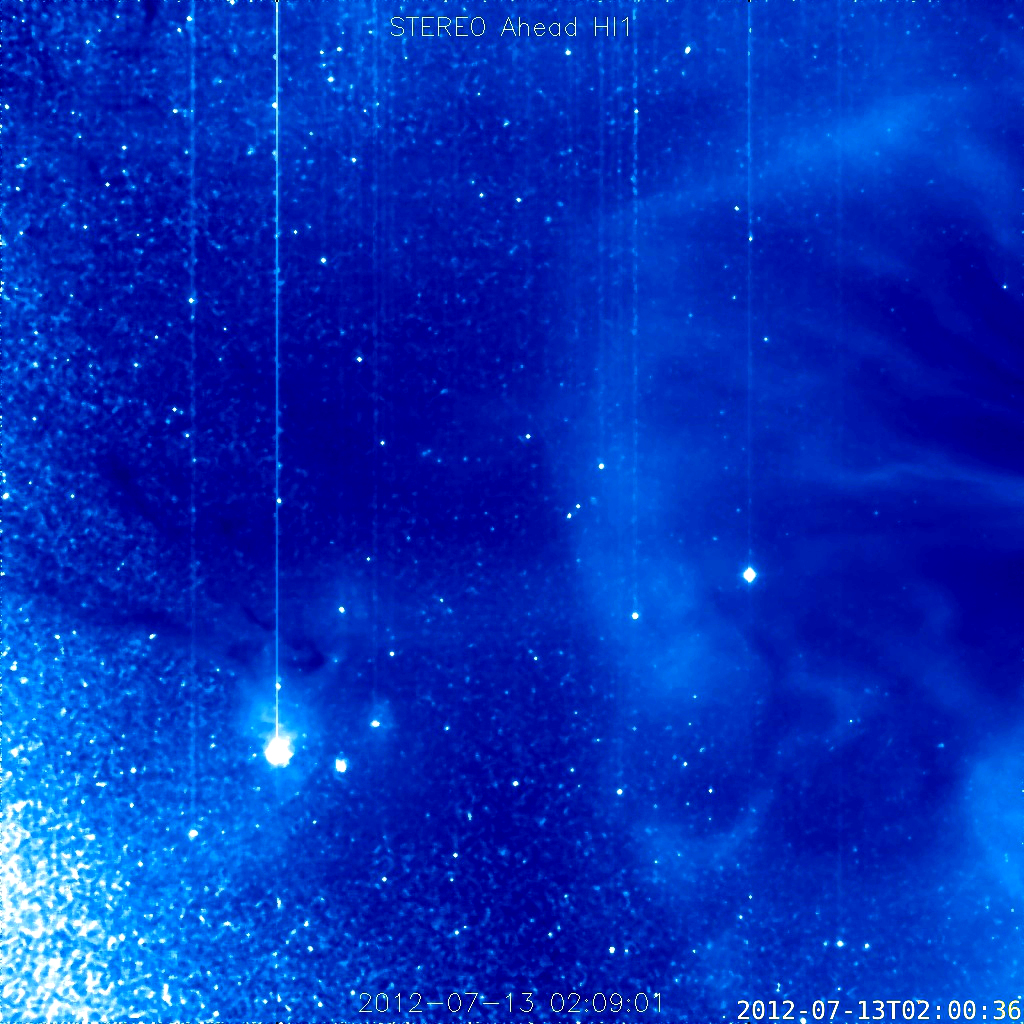
\includegraphics[width=0.99\textwidth]{figures/contributions/spaceweather/coronagraph.jpg}}
    \caption{The satellite image of HI 1.}
    \label{contributions:astro:spaceweather:rendering:coronagraph:coronagraph}
\end{subfigure}
\hspace*{1cm}
\begin{subfigure}[b]{0.32\textwidth}
    \fbox{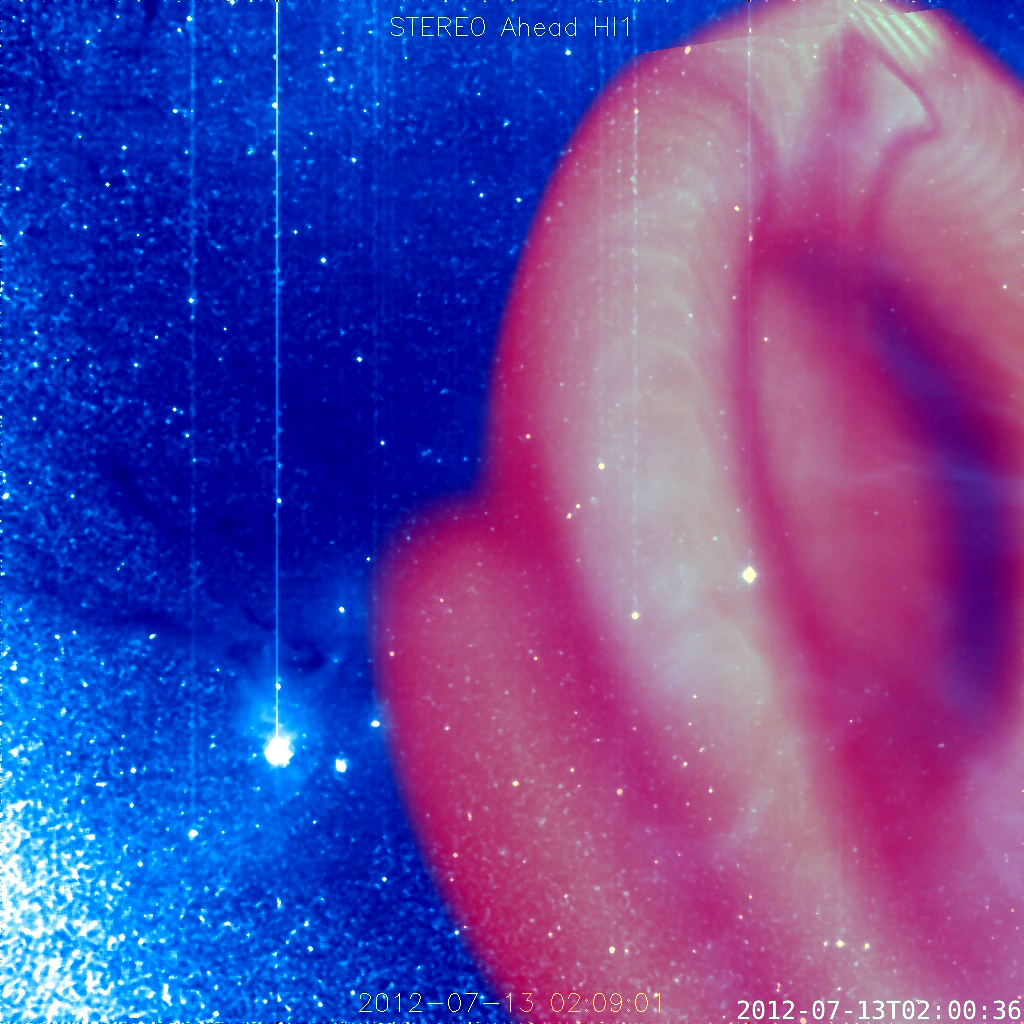
\includegraphics[width=0.99\textwidth]{figures/contributions/spaceweather/coronagraph_simulation.jpg}}
    \caption{Combined satellite image and simulation}
    \label{contributions:astro:spaceweather:velocity:coronagraph:coronagraph_simulation}
\end{subfigure}
\caption{The ability to control the transparency of satellite images is an important aspect in allowing the user to compare the predictions of the simulation to the acquired ground-truth images.}
\label{contributions:astro:spaceweather:rendering:coronagraph}
\end{figure}

The rendering employed in this application is mixing opaque geometry of solar system bodies, transparent satellite images, with multivolume raycasting.  One of the important technical aspect of this is the accurate positioning of all objects inolved in the scene have to be accurately positioned.  For the Earth, the Sun, and the involved satellites (STEREO A, STEREO B, and SOHO), we make use of the SPICE library that is provided by NASA's Navigation and Ancillary Information Facility~\cite{acton1996ancillary}.  The volumetric simulation, on the other hand, is provided in the \texttt{HEEQ} coordinate system, which uses the Sun's rotation axis and the vector between Sun and Earth at a specific epoch and constructs a right handed coordinate system from this.  With this information it is possible to compute a model matrix that orients the volume correctly in relation to the other scene elements.

\begin{wrapfigure}{o}{0.4\textwidth}
\centering
\fbox{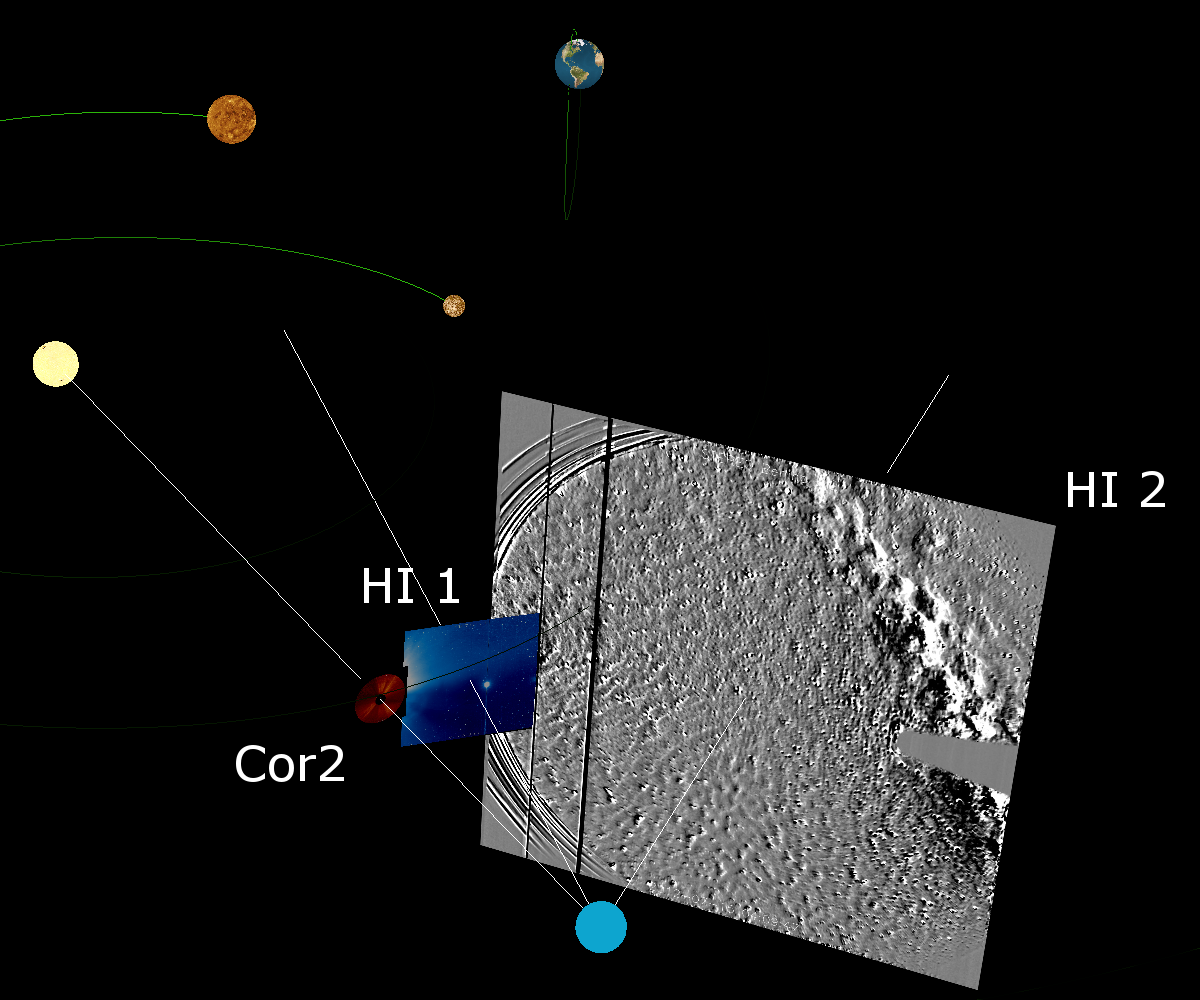
\includegraphics[width=0.38\textwidth]{figures/contributions/spaceweather/image_plane.png}}
\caption{Orientation of the various image planes.}
\label{contributions:astro:spacewather:rendering:planes}
\end{wrapfigure}

The satellite images are rendered along the view cone of the particular instrument.  The user can change the distance of the image plane from the satellite and thus its absolute size in the solar system (see \fref{contributions:astro:spacewather:rendering:planes}).  The image planes can be made semi-transparent, which enables the user to place the camera at the satellite's position and compare the image with the simulation result directly (see \fref{contributions:astro:spaceweather:rendering:coronagraph}).

For the volumetric rendering, we render two parameters that are included in the simulation.  During the development of this application, the scientists found that it was beneficial to perform each simulation twice; once without an injected CME to produce the background conditions, and once with the injected CME.  The volume rendering then uses the difference between the two values as a sample, thus only showing the effects of the CME while supressing the ambient background conditions.  The datasets are natively produced on a spherical grid which is stored as a regular structured \nD{3} cube on the GPU using $r$, $\phi$, and $\theta$ as the orthogonal coordinate axis, similar to Balabanian \etal \cite{balabanian2007sonar}.  The ray marching is performed in Cartesian coordinates, but for each sample location, these coordinates are converted into spherical coordinates before sampling the volume.  This has a number of beneficial characteristics.  The hardware trilinear interpolation that is performed on sampling in spherical coordinates produces the same results as a spherical linear interpolation, which is more beneficial for spherically symmetric datasets.  In addition, the non-uniform data distribution in Cartesian coordinates represents a crude basis for adaptive sampling, where there is a higher data density close to the Sun, where the CME is physically smaller.  Lastly, our volume rendering makes use of the spherical volume by employing geometry based entry space skipping.  Instead of using a bounding box to initiate the ray casting, we utilize a tesselated sphere instead and found the tesselation error to be negligble.

In order to support arbitrary ordering of, potentially, transparent geometry and volumetric rendering, improvements to the existing work of A-buffer implementations was developed that supports multiple volumes and multiple geometries in the same scene~\cite{lindholm14hybrid}.


\subsubsection{System} \label{contributions:astro:spaceweather:system}
The application consists of three separate views, the \emph{Ensemble View}~(see \SC{contributions:astro:spaceweather:system:ensemble}), the \emph{Timeline View}~(see \SC{contributions:astro:spaceweather:system:timline}), and the \emph{Spatial View}~(see \SC{contributions:astro:spaceweather:system:spatial}).  The \emph{Ensemble View} uses the glyph-based representation of ensemble members (see \SC{contributions:astro:spaceweather:glyphs}) and provides the user with an immediate view of the general trend of simulation accuracy.  The user can select individual ensemble members, which can then be inspected in the next view.  The \emph{Timeline View} shows the extracted velocities for each instrument for each spacecraft (see \SC{contributions:astro:spaceweather:opticalflow}) over time.  The user can inspect the extracted velocities at each time using the mouse and when selecting a time step, its datasets are loaded into the last view.  The \emph{Spatial View} makes use of the rendering algorithms described earlier (see \SC{contributions:astro:spaceweather:rendering}) in order to present a detailed view of the solarsystem's state at the selected time for the selected ensemble member.  Naturally, the locations and images of the satellites will be the same for all ensemble members, but the simluation results will be different.


\subsubsection{Evaluation} \label{contributions:astro:spaceweather:evaluation}
\begin{itemize}
    \item Weak point of the paper; no evaluation
    \item Everyone using exactly this system was involved in creating the system
    \item Example for benefit of close collaboration
\end{itemize}


\subsubsection{Generalization} \label{contributions:astro:spaceweather:generalization}
\begin{itemize}
    \item Generalization to any time-varying, volumetric ensemble simulation where an error function can be determined
\end{itemize}

\begin{landscape}
\begin{figure}
\centering
\begin{subfigure}[b]{0.4\textwidth}
    \fbox{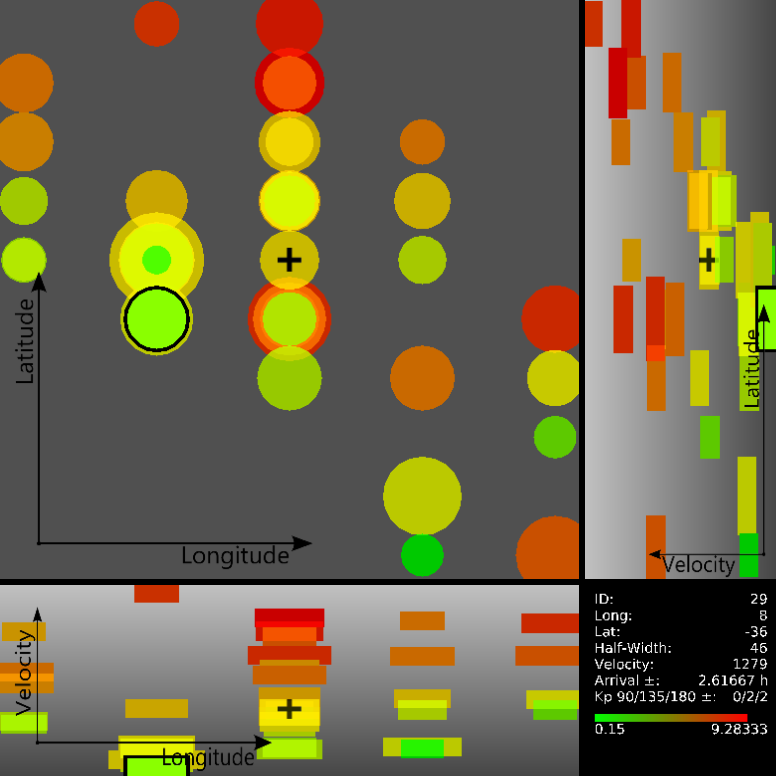
\includegraphics[width=0.99\textwidth]{figures/contributions/spaceweather/system-ensemble.png}}
    \caption{The \emph{Ensemble View} represents each member by a single glyph arranged in the four dimensional parameter space of \emph{longitude}, \emph{latitude}, \emph{opening angle}, and \emph{velocity}.}
    \label{contributions:astro:spaceweather:system:ensemble}
\end{subfigure}
\hfill
\begin{subfigure}[b]{0.4\textwidth}
    \fbox{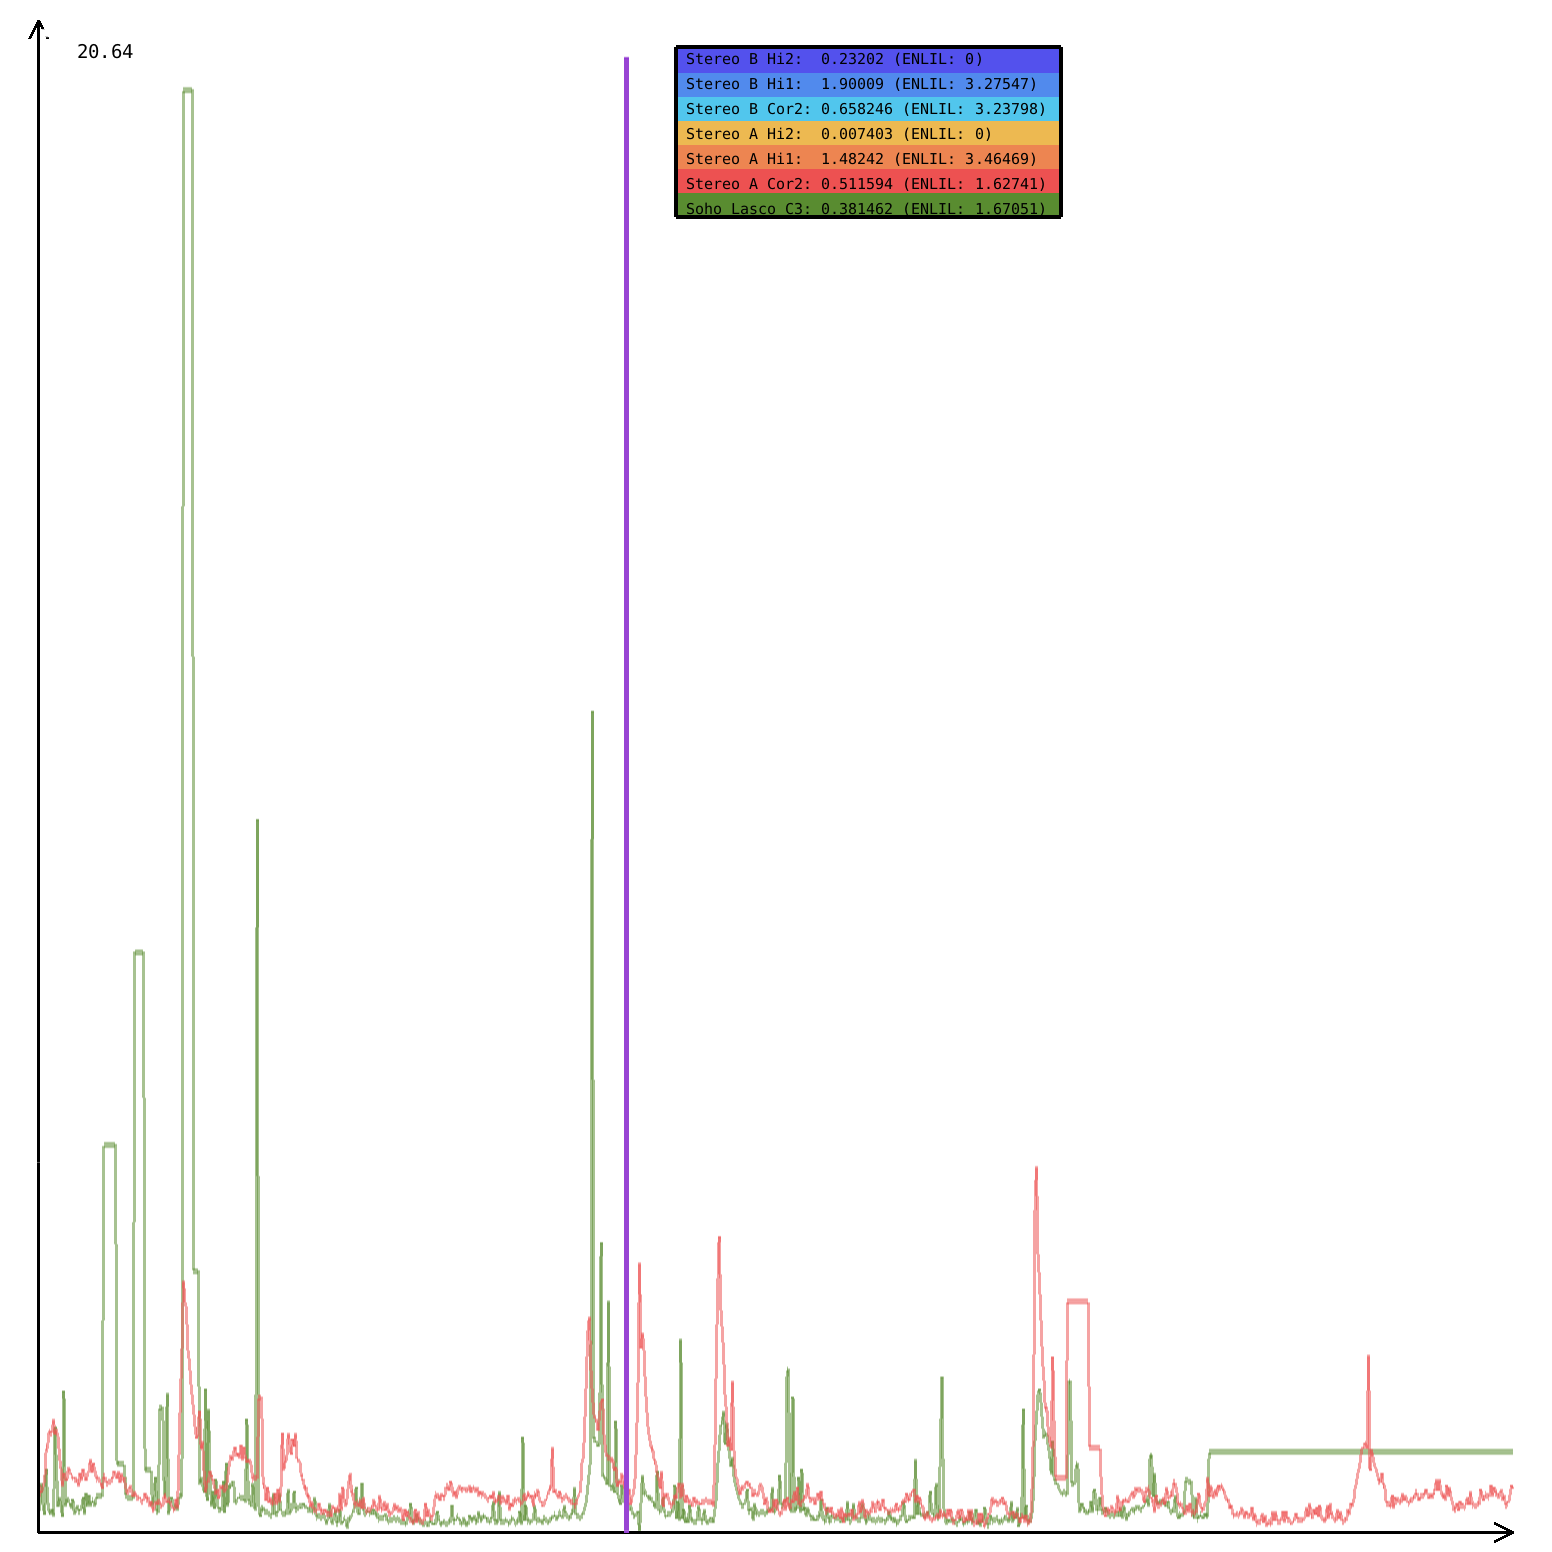
\includegraphics[width=0.99\textwidth]{figures/contributions/spaceweather/system-timeline.png}}
    \caption{The \emph{Timeline View} shows the development of a screen-space error metric over time and enables comparisons between satellite-acquired values and simulations results.}
    \label{contributions:astro:spaceweather:system:timeline}
\end{subfigure}
\hfill
\begin{subfigure}[b]{0.4\textwidth}
   \fbox{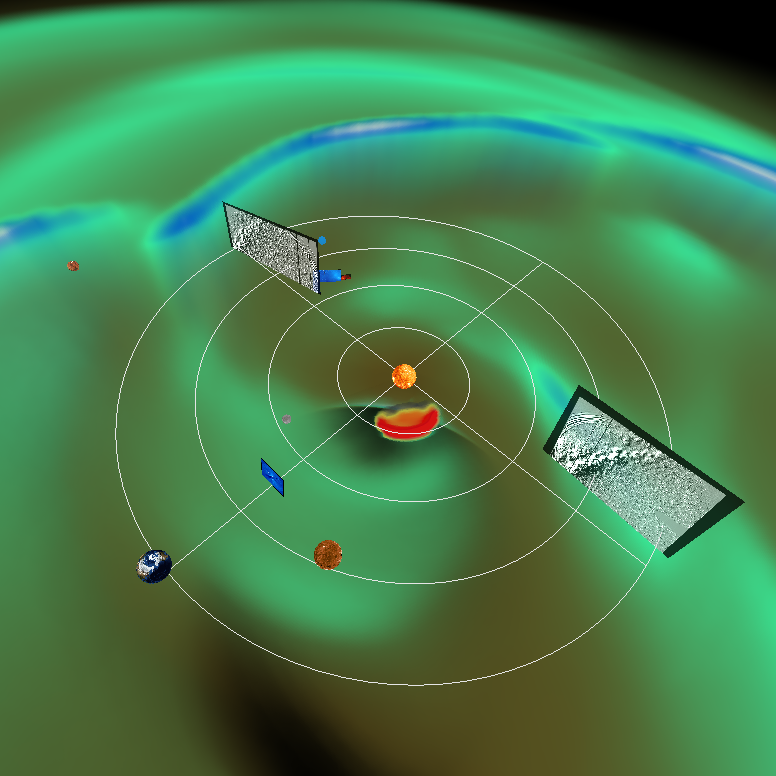
\includegraphics[width=0.99\textwidth]{figures/contributions/spaceweather/system-rendering.png}}
   \caption{The \emph{Spatial View} enables the user to inspect the results in a \nD{3} environment in which the satellite images are rendered accurately in relation to the simulation data.}
   \label{contributions:astro:spaceweather:system:rendering}
\end{subfigure}
\caption{An overview of the three components of the system presented in \paperef{paperF}, the user is presented with a full overview of the results of the ensemble data (a) in which they can select an ensemble member and get access to the detailed error timeline (b).  This view then user to inspect a specific timestep of the selected ensemble member in the contextualized spatial view (c) that includes a volumetric rendering of the simulation as well as the accurate location of the projected satellite images.}
\label{contributions:astro:spaceweather:system}
\end{figure}
\end{landscape}


\subsection{OpenSpace} \label{contributions:astro:openspace}
The \emph{OpenSpace} project was started in 2014 with the goal of created a freely available open-source software that can leverage synergies between three aspects of visualization in the context of astronomical visualization.  These aspects are the availability of the tool as a research tool for domain scientists for hypothesis generation and validation, its usage as a research platform for development of novel visualization research, and as a means to support the public dissemination of scientific discoveries.  By combining all three of these aspects into a single software platform, it becomes possible to shorten the deployment cycle of new visualization methods into the hands of domain scientists and the general public alike.  At the same time, it allows the domain scientists an avenue to quickly disseminate their research findings to the general public as well.  An additional benefit of providing all of these developments in a single platform is the ability to display distinct discoveries in their proper context, for example by showing the articulations of a surface rover on Mars in its correct environment, which was reconstructed from the images of orbiting satellites, or being able to present the movements of a space craft in the solar system while providing the image of the milky way and correctly aligned stars in the background as a reference point for the experts and to  increase immersion for the general public.

In order to support this effort, the software targets a variety of display systems, such as home computers, virtual reality headsets, and multi-pipeline display systems like planetarium domes or powerwalls.  This flexibility is one of the enabling factors to shorten the deployment cycle between the three pillars of the application as reasearchers, in most cases, do not have to invest any time to convert their data or algorithms to switch between any of the display modalities.

This ongoing effort were published in Papers~\ref{pa:paperG}, \ref{pa:paperH}, and \ref{pa:paperI} and is described in the rest of this section.  \paperef{paperG} describes the development of a dynamic scene graph that enables the display of objecst across large scales (see \SC{contributions:astro:openspace:dsg}).  \paperef{paperH} describes efforts on creating a system for a high-fidelity rendering system of planetary surfaces that support up to micrometer resolutions in order to be able to display geo-spatial discoveries in their correct spatial context (see \SC{contributions:astro:openspace:globebrowsing}).  Finally, \paperef{paperI} presents a higher level overview of the entire system to date.

\subsubsection{Dynamic Scene Graph} \label{contributions:astro:openspace:dsg}
One major feature of OpenSpace is the ability to display every available dataset in a single common reference frame in their correct context.  This necessitates the ability to express the location objects across enormous scale differences and provide the ability to render these simultaneously.  One example of this is the ability to render an Earth-orbiting satellite while also seeing the Cosmic Microwave Background radiation as the edge of the Observable Universe, a scene that coveres a scale difference of $10^26\,$m.  The usefulness of portraying these scale differences can be seen in the \emph{Powers of Ten} animation by Eames and Eames~\cite{morrison1982powers}.

One intrinsic difficulty of handling these vast scale differences is embedded into the traditional way of organizing a scene through a \emph{scene graph} by contructing a directed, acylcic graph that described a hierarchy of individual nodes where each node's position is expressed relative to its parent's position.  The camera position is expressed relative to the root node of the scene graph, which provides a problem if the camera is pointed at an object that is far away from the coordinate origin as the construction of the view matrix in this case might lead to catastrophic cancellation.

\paperef{G} addresses the issue 
\begin{itemize}
    \item Floating point precision error
    \item Take interval arithmetic from appendix of the paper
    \item Camera attached to a single object and traverse the scene graph from there
    \item Alternative way of thinking:  Dynamically rearrange the scene graph so that the camera-attached object is always at the root, including to invert transformations
\end{itemize}

\subsubsection{Planetary Rendering} \label{contributions:astro:openspace:globebrowsing}
\begin{itemize}
    \item Arbitrary planetary surfaces (triaxial ellipsoid)
    \item Get references from The Book
    \item Algorithm based on chunked Level-of-detail by Cozzi and Ring \cite{cozzi20113d} and Ulrich \cite{ulrich2002rendering}
    \item Color layers, height layers, water masks, night layers, overlay layers
    \item Possibility for temporal datasets for all layers
    \item Display of planetary surface detail Earth + Moon + Mars
    \item Public presentation (NASA Goddard, Ben Cook) in Hayden
    \item Bathymetry data (Hackathon)
    \item Glacial movement data (integrating radar measurements with global heightmap)
\end{itemize}

\subsubsection{Space Craft Missions} \label{contributions:astro:openspace:spacecraft}
\begin{itemize}
    \item Image projection by Everitt \cite{everitt2001hardware}
    \item Vis Poster\cite{bock15openspace}
    \item AGU presentation \cite{bock15bopenspace}
    \item New Horizons
    \item Rosetta
    \item Osiris-REx
    \item Hackathon
    \begin{itemize}
        \item Messenger
        \item Cassini
    \end{itemize}
\end{itemize}
